



%----------------  INTRODUCTION with THESIS STATEMENT ----------------------
\chapter{Introduction}
\label{chapter:intro}

In this chapter we will provide a more comprehensive analysis of the existing research surrounding ladder lotteries. Let {\sc x} be 
a ladder lottery or permutation. 
Throughout this thesis a number of algorithms are presented. Many of these algorithms use the following auxiliary functions: 
\begin{enumerate}
    \item {\sc Print(x)}: Prints {\sc x}.
    \item {\sc Swap(x,y)}: Swaps {\sc x, y}.
    \item {\sc Sort(x)}: Sorts {\sc x} in ascending order.
    \item {\sc Sorted(x)}: Returns true if {\sc x} is sorted in ascending order, else returns false.
    \item {\sc Max(x)}: Returns the maximum element in {\sc x}.
    \item {\sc Min(x)}: Returns the minimum element in {\sc x}.
\end{enumerate}

The study of ladder lotteries as mathematical objects began in 2010, in the paper
Efficient Enumeration of Ladder Lotteries and its Application, written by Matsui, Nakada, Nakano Uehara and Yamanaka~\cite{A1}. 
In this paper the authors present the first algorithm for generating $OptL\{\pi\}$ for some  
arbitrary permutation $\pi$. Since this paper emerged, there have been 
a number of other papers written about ladder lotteries.
These papers include The Ladder Lottery Realization Problem,
Optimal Reconfiguration of Optimal Ladder Lotteries, 
Efficient Enumeration of all Ladder Lotteries with K Bars,
Coding Ladder Lotteries and
Enumeration, Counting, and Random Generation of Ladder Lotteries.
This thesis is also heavily influenced by Efficient Enumeration of Ladder Lotteries and its Application. Throughout Chapter 2, 
we elaborate on the aforementioned papers pertaining to ladder lotteries.




\section{Thesis Statement}
    This thesis provides three full, or partial, solutions to three problems related 
    to ladder-lotteries. The first of these problems is the so called counting problem, 
    which asks, how many ladders are in $OptL\{\pi\}$? This thesis provides 
    a formula for the exact number of ladders in $OptL\{\pi\}$, for certain 
    cases of $\pi$ as well as a general recurrence relation for $OptL\{\pi\}$
    when $\pi$ is the decending permutation. The second problem is the so called canonical ladder listing problem. 
    This problem asks, given all permutations of size $N$, is there an algorithm 
    to list a canonical ladder from each permutation's $OptL\{\pi\}$? In other words, 
    is there an easy way to transition from one permutation's canonical ladder to the next 
    permutation's canonical ladder until all permutations of size $N$ have had their canonical 
    ladder generated? This thesis provides two such algorithms.The third problem is the so called minimum height 
    problem which asks, given all the ladders in $Optl\{\pi\}$, which ladder(s) are 
    the shortest, that is to say which ladders have the smallest height? Furthermore, given some arbitrary $\pi$, 
    is there a way to create a ladder for $\pi$ with minimal height? This thesis 
    provides an upper and lower bound for the minimal height of ladders along with a heuristic algorithm 
    for creating a ladder with minimal height.
   
\section{Overview of Thesis}  

This thesis is broken down into several sections. Firstly, an introuduction to Amidakuji, 
and how they pertain to computer science will be presented. This will be followed by a literature 
review of ladder lotteries in which discussions of solved problems will be 
provided, along with the commonalities between ladder lotteries and 
other mathematical objects. Following the literature review, three chapters pertaining to the three problems will be 
provided. In each of these three chapters there is an introduction to the problem, a methodology section, a results 
section and a conclusion section. The introduction section introduces the problem to the reader, providing the necessary 
definitions and concepts. The methodology sections contain the algorithms and formulas used to solve the respective problems. 
Following the methodology sections, the results generated by the algorithms and formulas will be presented.
In the results sections there will be proofs and formulas for certain propositions made in regards to the respective problems. 
Following the results section, an analysis of the results will be presented along with a summary  of future pertaining to the problem 
will be provided. In this section,
the failures and successes of this research will be analyzed. There will also be commentary on 
open (unsolved) problems related to ladder lotteries and a 
discussion of how research on ladder lotteries could be used in other fields.
Finally, a conlcusion that summarizes the thesis will be provided.

%----------------  BACKGROUND and LITERATURE REVIEW ----------------------
\chapter{Background and Literature Review}
\label{chapter:background}
An interesting property about ladder lotteries is that they can be derived from a 
\emph{permutation} which is a is a unique ordering of objects.
For the purposes on this paper, the objects of a permutation will be integers 
ranging from [$1$ $\dots$ $N$]. \emph{Optimal ladder lotteries} are a special case of ladder 
lotteries in which there is one bar in the ladder for each \emph{inversion} in the permutation.
An \emph{inversion} is a relation between two elements in $\pi$, 
$\pi_{i}$ and $\pi_{j}$, such that if $\pi_{i}>\pi_{j}$ and $i<j$ then $\pi_{i}$ and $\pi_{j}$ 
form an inversion. 
For example, given $\pi=(4,3,5,1,2)$, its iversion set is $Inv(\pi) =\{(4,3),(4,1),(4,2),(3,1),(3,2),(5,1),(5,2)\}$.
Every permutation has a unique, finite set of optimal ladder lotteries associated with it. 
 Thus, the set of optimal ladder lotteries associated with $\pi$, 
 hereby known as \emph{$OptL\{\pi\}$}, is the set containing all ladder lotteries 
 with a number of bars equal to the number if inversions in $\pi$. 
 See Fig. 2.1 for an example of an optimal ladder in $OptL\{(4,3,2,1)\}$.
 For each optimal ladder in $OptL\{\pi\}$, the $N$ 
 elements in $\pi$ are listed at the top of a ladder and each 
 element is given its own line. 
 At the bottom of a ladder is the \emph{sorted permutation}, 
 hereby known as the \emph{identity permutation} \cite{A7}. 
 The  identity permutation of size $N$ is defined as follows - $I:(1, 2, 3, \dots, N)$. 
 Each ladder in $OptL\{\pi\}$ has the minimal number of horizontal bars to sort $\pi$ 
 into the identity permutation. Each bar in a ladder from $OptL\{\pi\}$ uninverts a single 
 inversion in $\pi$ exactly once. For the remainder of this paper, only optimal ladder 
 lotteries will be discussed, with one exception. Therefore when the term ladder lottery is used, assume 
 optimal ladder lottery unless otherwise stated.\par
 
\begin{figure}[!htp]
    \label{fig:ab}
	\begin{minipage}{0.4\textwidth}
		\centering
		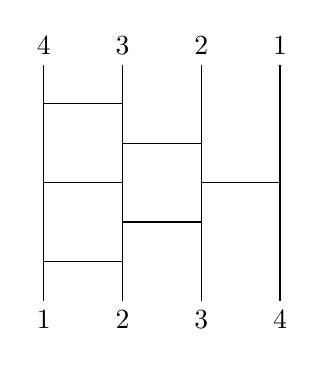
\begin{tikzpicture}
		 	\draw(0, 0) to (0, 3) ++(0, 0) node[above]{4} --(0, 0)node[below]{1};
		 		\draw(0, 2.5) to (1, 2.5);
		 		\draw(0, 1.5) to (1, 1.5);
		 		\draw(0, 0.5) to (1, 0.5);

		 	\draw(1, 0) to (1, 3) ++(0, 0) node[above]{3} --(1, 0)node[below]{2};
		 		\draw(1, 2) to (2, 2);
		 		\draw(1, 1) to (2, 1);
		 	\draw(2, 0) to (2, 3) ++(0, 0) node[above]{2} --(2, 0)node[below]{3};
		 		\draw(2, 1.5) to (3, 1.5);
		 	\draw(3, 0) to (3, 3) ++(0, 0) node[above]{1} --(3, 0) node[below]{4};
		\end{tikzpicture}
				

	\end{minipage}
	\begin{minipage}{.4\textwidth}
		\begin{flushright}
		
		
		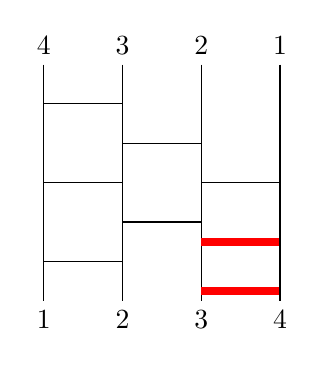
\begin{tikzpicture}
		 	\draw(0, 0) to (0, 3) ++(0, 0) node[above]{4} --(0, 0)node[below]{1};
		 		\draw(0, 2.5) to (1, 2.5);
		 		\draw(0, 1.5) to (1, 1.5);
		 		\draw(0, 0.5) to (1, 0.5);
		 		

		 	\draw(1, 0) to (1, 3) ++(0, 0) node[above]{3} --(1, 0)node[below]{2};
		 		\draw(1, 2) to (2, 2);
		 		\draw(1, 1) to (2, 1);
		 	\draw(2, 0) to (2, 3) ++(0, 0) node[above]{2} --(2, 0)node[below]{3};
		 		\draw(2, 1.5) to (3, 1.5);
		 		\draw[line width=1mm, red](2, 0.75) to (3, 0.75);
		 		\draw[line width=1mm, red](2, 0.125) to (3, 0.125);
		 	\draw(3, 0) to (3, 3) ++(0, 0) node[above]{1} --(3, 0) node[below]{4};
		\end{tikzpicture}
	\end{flushright}
	\end{minipage}
	\caption{Two ladders for the permutation (4, 3, 2, 1). The left ladder is an optimal ladder and the right ladder is not. Therefore the left ladder belongs to $optL\{(4,3,2,1)\}$. The bold  bars in the right ladder are redundant, thus the right ladder is not optimal}
	
\end{figure}


 


\chapter{Literature Review}
%%Intro to the Literature Review
\subsection{Literature Overview}
    The study of ladder lottieres as mathematical objects began in 2010, in  the paper
    \textbf{Efficient Enumeration of Ladder Lotteries and its Application}. The paper was 
    written by four authors, Yamanaka, Horiyama, Uno and Wasa. In this paper the 
    authors present an algorithm for generating all the ladder lotteries of an 
    arbitrary permutation, $\pi$. Since this paper emerged, there have been 
    several other paper written directly about ladder lotteries. 
    These papers include \textbf{The Ladder Lottery Realization Problem},
    \textbf{Optimal Reconfiguration of Optimal Ladder Lotteries}, 
    \textbf{Efficient Enumeration of all Ladder Lotteries with K Bars},
    \textbf{Coding Ladder Lotteries} and
    \textbf{Enumeration, Counting, and Random Generation of Ladder Lotteries}.

%$input review of first paper
\section{Efficient Enumeration of Laddder Lotteries and its Application}

%%Intro
\subsection{Introduction}
In their paper, \textbf{Efficient Enumeration of Ladder Lotteries and its Application},
the authors provide an algorithm for generating $OptL\{\pi\}$ 
for any $\pi$, in $\mathcal{O}(1)$ per ladder \cite{A1}. This is the first algorithm for generating $OptL\{\pi\}$. 
To see this algorithm please refer to 
Alg.\ref{Alg:FindAllChildren}. The paper also presents the number 
of ladder lotteries in $OptL\{(11, 10, 9, 8, 7, 6, 5, 4, 3, 2, 1)\}$ which is 
$5,449,192,389,984$ \cite{A1}.There are also four other algorithms in 
this section, none of which are found in the paper \emph{Efficient Enumeration of Ladder Lotteries and its Applications}. The 
algorithms are Alg.\ref{Alg:RootLadder}, Alg.\ref{Alg:RightSwap}, Alg.\ref{Alg:LeftSwap} and Alg.\ref{Alg:ShiftChildren}.
These algorithms are used to perform mandatory steps in \ref{Alg:FindAllChildren}. These algorithms are novel.\par 
The authors' algorithm is known as \emph{FindAllChildren}. It is based on several key concepts, the most 
important of which is the \emph{local swap operation}. This is the 
minimal change operation that transitions from one ladder in $OptL\{\pi\}$ to the 
next ladder. The local swap operation is essentially a 180 degree rotation
of three bars in the ladder, such that the bottom
bar is rotated to the top, the middle bar stays in the middle and the top bar
is rotated to the bottom. If the bars undergo a 180 degree rotation to the right, 
then this is known as a \emph{right swap operation} and 
if the bars udergo a 180 degree rotation to the left then this 
is known as a \emph{left swap operation} \cite{A1}. To go to the next ladder in the set, 
the current ladder, $l_{i}$, udergoes a right swap operation 
to get to ladder $l_{i+1}$. See Fig.\ref{fig:rightSwap} for an exmaple of a 
local swap operation. The \emph{route} of an element is the sequence of bars in the ladder that an element must cross 
in order to reach its correct position in 
the identity permutation \cite{A1}. The sequence is ordered from top left to bottom right.
Note, that each bar has two elements that cross it, 
therefore the bar belongs to the route of the greater of the two elements. 
It is important to note that when a right swap operation occurs, 
two of the three bars belong to the route of a unique greater element and one bar belongs
to the route of a unique lesser element. Once rotated, the bar of the lesser element is 
moved above the bars of the greater element.\par
The \emph{clean level} refers to the smallest element 
in $\pi$ such that none of its bars have undergone a right swap operation \cite{A1}.
If there is no such element, then the clean level is the maximum element in $\pi$ + 1.
The \emph{root ladder} is the only ladder in  the set with a clean level of 1; in 
other words, the root ladder is the only ladder in which no bars have undergone 
a right swap operation. The root ladder is unique to $OptL\{\pi\}$. To see the root ladder 
of $OptL\{(4,5,6,3,1,2)\}$ please refer to figure Fig.\ref{fig:root}. The root ladder is
also the \emph{first ancestor  ladder} in $OptL\{\pi\}$. Insofar as the enumeration algorithm 
is based on performing a right swap operation on a pervious ladder, then every other 
ladder in $OptL\{\pi\}$ must have at least one right swap operation. Since the root ladder has
no right swap operations, then it must be an ancestor of every other ladder.\par

%%Root ladder subsection
\subsection{The Root Ladder in Detail}
The authors provide a good description of the root ladder, however they do not provide an algorithm 
for creating the root ladder. Since the root ladder is an ancestor to every other ladder in $OptL\{\pi\}$, 
the root ladder cannot be created using the same algorithm as every other ladder. This thesis provides such 
an algorithm in Alg.\ref{Alg:RootLadder}.\par

\begin{algorithm}
	%%\setstretch{1.35}
	 %% \algsetup{linenosize=\tiny}
	\begin{algorithmic}[1]
		\Function {CreateRoot}{$ladder[2(N-1)-1][N-1]$, $\pi$, $N$, $row \gets 1$}
			\If{$N=1$}
				\State return
			\EndIf
			\State $largestIndex \gets$ index of largest element in $\pi$
			\For{$i \gets largestIndex+1$, $i \leq N$, $i \gets i+1$}
				\If{$\pi_{largestIndex}>\pi_{i}$ $AND$ $largestIndex < i$}
					\State $column \gets i$
					\If{This is the first bar to be added}
						\While{bar cannot be added}
							\State $row \gets row+1$
						\EndWhile
						\State $ladder[row][column] \gets 1$
					\Else 
						\State $row \gets row+1$
						\State $ladder[row][column] \gets 1$
					\EndIf
				\EndIf
			\EndFor
			\State $\pi \gets \pi - largestElement$
			\State $CreateRoot(ladder, \pi, N-1, row \gets 1)$
		\EndFunction

	\end{algorithmic}
	\caption{The algorithm for creating the root ladder of $OptL\{\pi\}$}
	\label{Alg:RootLadder}
\end{algorithm}\pagebreak



Let $ladder$ be a two dimensional array, let $\pi$ be the current state of the permutation, let $N$ be the 
size of $\pi$, let $row$ be the current row in the ladder. First, the index of the largest element in $\pi$ is assigned to $largestIndex$. 
Once found, the algorithm loops from $largestIndex+1$ to $N$. If $\pi_{largestIndex}>\pi_{i}$ then a bar is to be added to 
$ladder$ at $row,column=i$. There are two cases for calculating the $row$. 
\case{\emph{First bar is being added}}{This is the first bar to be added to the route of the largest element. 
$row$ is incremented until a bar can be added to $ladder$ at $row$ 
and $column$. A bar can be added if neither of its endpoints are touching the endpoints of any other bar.}
\case{\emph{Second or greater bar is being added}}{If this is second or greater bar to be added to the route of the 
largest element in $\pi$ then $row \gets row+1$.}
Once all the bars for the route of the largest element have been added, the largest element from $\pi$ is removed, 
$N \gets N-1$ and $row \gets 1$. Then the algorithm makes a recursive call.

\begin{lemma}
	The time complexity for $CreateRoot$ is $O(N^{3})$
\end{lemma}
\begin{proof}
	The outer for-loop of the function runs from some arbitrary index to $N$ on each function call. The inner for loop runs at most 
	$2(N-1)-1$ times which is reduced to $N$. Thus, we get $O(N^{2})$. The following 
	recursion holds, $CreateRoot(N-K) = CreateRoot(N-K+1) + O((N-K)^{2})=CreateRoot(N-K+2) + O((N-K)^{2}) + O((N-K+1)^{2})\dots $. Which is 
	reduced to $O(N(N+1)(2N+1)/6) = O(N^3)$. QED.
\end{proof}
\pagebreak


\begin{figure}[!htp]
	\begin{minipage}{0.4\textwidth}
		\begin{center}

			%%drawing the lines
			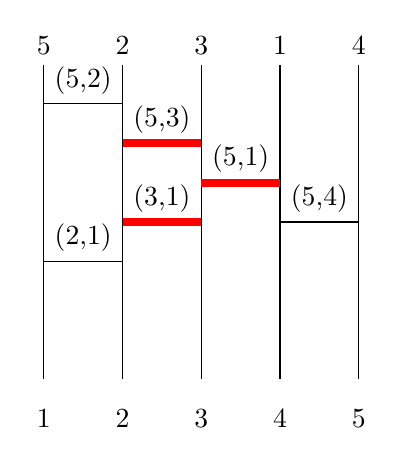
\begin{tikzpicture}
				\draw(0, 0) to (0, 4) node[above]{5};
				\node at (0, -0.5){1};

				\draw(1, 0) to (1, 4) node[above]{2};
				\node at (1, -0.5){2};


				\draw(2, 0) to (2, 4) node[above]{3};
				\node at (2, -0.5){3};

				\draw(3, 0) to (3, 4) node[above]{1};
				\node at (3, -0.5){4};


				\draw(4, 0) to (4, 4) node[above]{4};
				\node at (4, -0.5){5};

				%%drawing the bars

				%%5's route
				\draw(0, 3.5)to (1, 3.5);
					\draw node at (0.5, 3.8) {(5,2)};
				\draw[line width=1mm, red](1, 3) to (2, 3);
					\draw node at (1.5, 3.3) {(5,3)};
				\draw[line width=1mm, red](2, 2.5) to (3, 2.5);
					\draw node at (2.5, 2.8) {(5,1)};
				\draw(3, 2) to (4, 2);
					\draw node at (3.5, 2.3) {(5,4)};

				%%4's route, no bars

				%%3s route
				\draw[line width=1mm, red](1, 2) to (2, 2);
					\draw node at (1.5, 2.3) {(3,1)};
				%%2s route
				\draw(0, 1.5) to (1, 1.5);
					\draw node at (0.5, 1.8){(2,1)};
			\end{tikzpicture}
		\end{center}
	\end{minipage}
	\begin{minipage}{0.4\textwidth}
		\begin{flushright}

			%%drawing the lines
			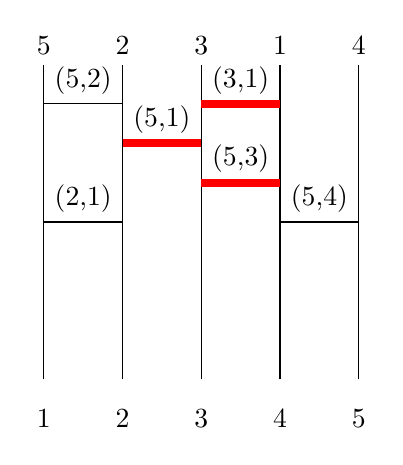
\begin{tikzpicture}
				\draw(0, 0) to (0, 4) node[above]{5};
				\node at (0, -0.5){1};

				\draw(1, 0) to (1, 4) node[above]{2};
				\node at (1, -0.5){2};


				\draw(2, 0) to (2, 4) node[above]{3};
				\node at (2, -0.5){3};

				\draw(3, 0) to (3, 4) node[above]{1};
				\node at (3, -0.5){4};


				\draw(4, 0) to (4, 4) node[above]{4};
				\node at (4, -0.5){5};

				%%Drawing the bars
				\draw(0, 3.5)to (1, 3.5);
					\draw node at (0.5, 3.8){(5,2)};
				\draw[line width=1mm, red](2, 3.5) to (3, 3.5);
					\draw node at (2.5, 3.8) {(3,1)};
				\draw[line width=1mm, red](2, 2.5) to (3, 2.5);
					\draw node at (2.5, 2.8) {(5,3)};
				\draw(3, 2) to (4, 2);
					\draw node at (3.5, 2.3){(5,4)};
				%%4's route, no bars

				%%3s route
				\draw[line width=1mm, red](1, 3) to (2, 3);
					\draw node at (1.5, 3.3) {(5,1)};
				%%2s route
				\draw(0, 2) to (1, 2);
					\draw node at(0.5, 2.3){(2,1)};
			\end{tikzpicture}
		\end{flushright}
	\end{minipage}
	\caption{Example of a local swap operation. When a right swap operation is permformed
	on the left ladder, the result is the right ladder. When a left swap operation is permformed
	on the right ladder, the result is the left ladder.}
	\label{fig:rightSwap}
\end{figure}


\begin{figure}


	\begin{center}
		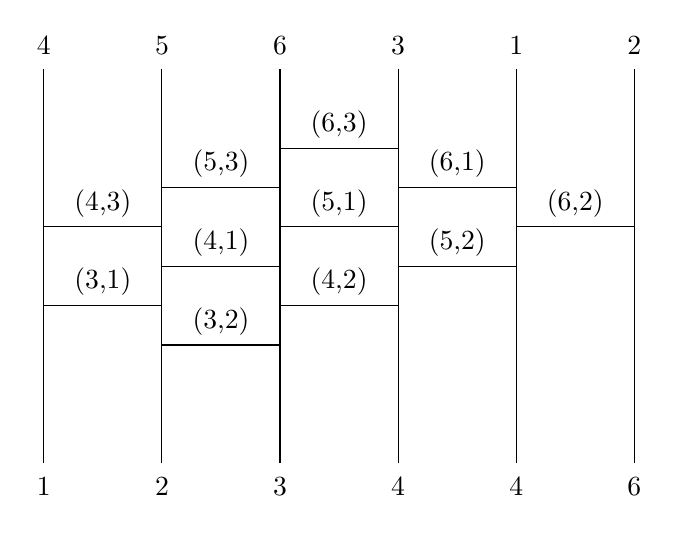
\begin{tikzpicture}
			%%draw the lines
			\draw(0, 0) to (0, 5);
				\node at (0, 5.3){4};
				\node at (0, -0.3){1};

			\draw(1.5, 0) to (1.5, 5);
				\node at (1.5, 5.3){5};
				\node at (1.5, -0.3){2};
			
			\draw(3, 0) to (3, 5);
				\node at (3, 5.3){6};
				\node at (3, -0.3){3};
			\draw(4.5, 0) to (4.5, 5);
				\node at (4.5, 5.3){3};
				\node at (4.5, -0.3){4};
			\draw(6, 0) to (6, 5);
				\node at (6, 5.3){1};
				\node at (6, -0.3){4};
			\draw(7.5, 0) to (7.5, 5);
				\node at (7.5, 5.3){2};
				\node at (7.5, -0.3){6};

			%%draw the bars
			
			%%6's route
			\draw(3, 4) to (4.5, 4);
				\node at (3.75, 4.3){(6,3)};
			\draw(4.5, 3.5) to (6, 3.5);
				\node at (5.25, 3.8){(6,1)};
			\draw(6, 3) to (7.5, 3);
				\node at (6.75, 3.3){(6,2)};
			%%5's route
			\draw(1.5, 3.5) to (3, 3.5);
				\node at (2.25, 3.8){(5,3)};
			\draw(3, 3) to (4.5, 3);
				\node at (3.75, 3.3){(5,1)};
			\draw(4.5, 2.5) to (6, 2.5);
				\node at (5.25, 2.8){(5,2)};
			%draw 4's route
			\draw(0, 3) to (1.5, 3);
				\node at (0.75, 3.3){(4,3)};
			\draw(1.5, 2.5) to (3, 2.5);
				\node at (2.25, 2.8){(4,1)};
			\draw(3, 2) to (4.5, 2);
				\node at (3.75,2.3){(4,2)};

			%%draw 3's route
			\draw(0, 2) to (1.5, 2);
				\node at (0.75, 2.3){(3,1)};
			\draw(1.5, 1.5) to (3, 1.5);
				\node at (2.25, 1.8){(3,2)};
		\end{tikzpicture}

	\end{center}





	\caption{The root ladder for $OptL\{(4,5,6,3,1,2)\}$. Notice how 
	none of the bars have undergone a right swap operation. This is clear 
	when considering that there is no bar of a lesser element above the bar(s)
	of a greater element.} 
	\label{fig:root}

\end{figure}

 %%Save this section for the counting section.
 \begin{theorem}
	 If a ladder from $OptL\{\pi\}$ has not undergone any right swap operations then the ladder is the root ladder. 
	 \label{Theorem:One}
 \end{theorem} 
 \begin{proof}
     The root ladder is defined as the ladder whose clean level is one.
     This means there is no bar of a lesser element above the route a 
     greater element. Keeping in mind that the clean level of the root ladder is one, next consider what is meant by a \emph{child bar}
      which is a bar to the bottom left or right of an arbitrary bar $x$. Within the context of the root ladder, 
      if the left endpoint of the child bar is directly below the right end point of $x$ then the child is a 
     \emph{right child} of $x$. If the right end point of the child bar is directly 
     below the left end point of $x$ then it is a \emph{left child}. Let $x$ belong to the route of element $m$/$Route(m)$.
     If a child is a right child of $x$
	 then it also belongs to the $Route(m)$.
     Let $x$ be a bar representing an inversion with element $m$ and $k$.
     The right child of $x$ is a bar which represents an inversion 
     with $m$ and some element to the right of $k$ termed $k'$. Suppose this was not the case, 
     then this would mean that the right child of $x$ was either a bar representing an inversion 
	 between some element $m'$ such that $m' > m$ or $m' < m$. If $m' > m$ 
	 then this would be a contradiction seeing as $x$ would be above the bar of a route 
     of a greater element which contradicts the definition of the root ladder. On the other hand if 
	 $m' < m$ then $m$ would form an inversion with $m'$ and $x$ would be the bar that uninverted $m$ and $m'$, 
	 but this is also a contradiction seeing as $m' \neq k$ but $x$ uninverts $m$ and $k$. Thus, the right child 
     of $x$ belongs to the same route as $m$ in the root ladder.\par The left child of $x$
     belongs to $Route(l=m-1)$. Suppose this was not the case, 
     then the left child could belong to a route $\geq m$, but if that were the case, this contradicts 
	 the definition of the root ladder seeing as $x$ would be above the route of a greater element. If 
	 $l < m-1$ then the left child of $x$ would be above $Route(m-1)$ which also contradicts the definition 
	 of the root ladder. Therefore, the left child of $x$ must belong to route $l=m-1$. 
	 The second element of the left child of $x$ is $k$. Suppose this was not the case, then 
	 let the second element of the left child be termed $k'$. 
	 $k'$ forms an inversion with $m-1$. But since $m-1 < m$ then $m$ would also form an inversion with $k'$, the 
	 bar corresponding to the inversion $m$ and $k'$ would be $x$. But we already stated that $x$ forms 
	 an inversion between $m$ and $k$, therefore we have another condtradiction. 
	 Therefore, the second element of left child of $x$ must be $k$; the left child of $x$ uninverts elements 
	 $m-1$ and $k$. \par 
	 Please refer to Fig. \ref{Fig:RootChildBars} to view an example of the root ladder for $(3,1,5,2,4)$. Note 
	 that this is a figure of the only ladder in $OptL\{(3,1,5,2,4)\}$.
	 By that the right/left children bars of any given bar 
	 $x$ have not been right swapped, we have proven that if a ladder in $OptL\{\pi\}$ has not undergone 
	 a right swap operation then it must be the root ladder. QED\pagebreak

   
 \end{proof}
 \begin{corollary}
	 If $|OptL\{\pi\}|=1$ then the ladder in $OptL\{pi\}$ must be the root ladder.
 \end{corollary}
 \begin{proof}
	 If there is only one ladder in the set, then that means no bars have been swapped in said ladder. 
	 Thus, it must be the root ladder. QED.
 \end{proof}


 \begin{figure}[!htp]
     \begin{center}
     \begin{tikzpicture}
         \draw(0, 0) to (0, 4);
             \node at(0, 4.3){$3$};
              \draw(0, 3.5) to (2, 3.5);
                 \node at(1, 3.8){$3,1$};
           
             \draw[line width=0.8mm, red](2, 2.5) to (4, 2.5);
                 \node at(3, 2.8){$3,2$};

         \draw(2, 0) to (2, 4);
             \node at(2, 4.3){$1$};
          
         \draw(4, 0) to (4, 4);
              \node at(4, 4.3){5};
                 \draw(4, 3.5) to (6, 3.5);
                     \node at (5, 3.8){$5,2$};
         \draw(6, 0) to (6, 4);
			 \node at(6, 4.3){2};
			 \draw[line width=0.8mm, red](6, 2.5) to (8, 2.5);
			 	\node at(7,2.8){$5,4$};

		\draw(8, 0) to (8, 4);
			\node at(8, 4.3){4};


     \end{tikzpicture}
     \end{center}
     \caption{The root ladder/only ladder in $OptL\{(3,1,5,2,4)\}$ Note that bar 4,2 is the parent of bar 3,2 and 4,1. Also note that 
	 bar 3,2 is the the left child of 4,2 and 4,1 is the right child.}
	 \label{Fig:RootChildBars}
 \end{figure}

%%algorithm
\subsection{$FindAllChildren$}

Let $ladder$ be initilaized as the root ladder. Let $CleanLevel$ be initilaized to $1$. 
Let $N$ be initialized to the max element. The enumeration algorithm 
lists $OptL\{\pi\}$; the authors refer to the algorithm as $FindAllChildren$ \cite{A1}. 
$FindAllChildren$ was used for the bulk of this research, however 
the authors omitted several key steps in the the algorithm. Most notably, they 
omitted the right/left swap operation. Nor do they provide an algorithm 
for permforming a right/left swap operation \cite{A1}. Therefore, I have provided 
the right and left swap operations.
To see $FindAllChildren$ for generating $OptL\{\pi\}$ please refer to Alg.\ref{Alg:FindAllChildren}.
 To see the right/left swap algorithms please 
refer to Alg.\ref{Alg:RightSwap} and Alg.\ref{Alg:LeftSwap} respectively. To 
see an example of a right/left swap operation please refer to Fig.\ref{fig:rightSwap}.
Given an arbitrary bar, $x$, it can be right swapped if and only if there are two bars, $y,z$ where $y \neq z$ 
such that all the following conidtions are met \cite{A1}.
\begin{itemize}
	\item The left end point of $z$ is directly above the left end point of $x$.
	\item The left end point of $y$ is directly above the right end point if $x$.
	\item The right end point of $z$ is directly above the left end point of $y$.
\end{itemize}

Given an arbitrary bar, $x$, it can be left swapped if and only if there are two bars, $y,z$ where $y \neq z$ 
such that the following conditions are met \cite{A1}.
\begin{itemize}
	\item The right end point of $z$ is directly below the right end point of $x$.
	\item The right end point of $y$ is directly below the left end point if $x$.
	\item The left end point of $z$ is directly below the right end point of $y$.
\end{itemize}
In the left ladder in Fig.\ref{fig:rightSwap} bar $x=(3,1)$, bar $y=(5,1)$ and bar $z=(5,3)$. Bar $x$ can be right swapped 
seeing as the three conditions for performing a right swap operation are met.
In the right ladder in Fig.\ref{fig:rightSwap} bar $x=(3,1)$, bar $y=(5,1)$ and bar $z=(5,3)$. Bar $x$ can be left swapped 
seeing as the three conditions for performing a left swap operation are met.


\begin{algorithm}
	\begin{algorithmic}[1]
		\Function{FindAllChildren}{$ladder$, $cleanLevel$, $N$}
			\State $currentRoute \gets N$
			\While{$currentRoute \geq cleanLevel$}
				\State going top left to bottom right 
				\For{$bar \in currentRoute$}
					\State $row \gets$ row of $bar$ in $ladder$ 
					\State $col \gets$ col of $bar$ in $ladder$
					\State $lowerNeighbor \gets ladder[row-1][col]$
					\If{$lowerNeighbor$ is right swappable}
						\State $RightSwap(ladder, bar, lowerNeighbor)$
						\State $FindAllChildren(ladder, y+1, N)$
						\State $leftSwap(ladder, bar, lowerNeighbor)$
					\EndIf
				\EndFor
				\State $currentRoute \gets currentRoute-1$
			\EndWhile
			\State $currentRoute \gets cleanLevel-1$
			\For{$bar \in currentRoute$}
				\State $row \gets$ row of $bar$ in $ladder$ 
				\State $col \gets$ col of $bar$ in $ladder$
				\State $lowerNeighbor \gets ladder[row-1][col]$
				\If{$lowerNeighbor$ is right swappable $AND$ is the rightmost bar of $currentRoute-1$}
					\State $RightSwap(ladder, bar)$
					\State $findAllChildren(ladder, cleanLevel, N)$
					\State $LeftSwap(ladder, bar)$
				\EndIf
			\EndFor
		\EndFunction
	\end{algorithmic}
	\caption{The algorithm for listing $OptL\{\pi\}$.}
	\label{Alg:FindAllChildren}
\end{algorithm}


\begin{algorithm}
	\begin{algorithmic}[1]
		\Function{RightSwap}{$ladder$, $bar$}
			\State $row \gets bar's$ row
			\State $col \gets bar's$ column
			\State $upperNeighbor \gets ladder[row-2][col]$
			\State $rightNeighbor \gets ladder[row-1][col+1]$
			\State $rightSibling \gets ladder[row][col+2]$
			\State $ShiftSubLadder(ladder, rightSibling, 2, 1)$
			\State $Swap(upperNeighbor, ladder[row+1][col+1])$
			\State $Swap(bar, rightNeighbor)$ 
		\EndFunction
	\end{algorithmic}
	\caption{Perform a right swap operation on a bar}
	\label{Alg:RightSwap}
\end{algorithm}
\begin{algorithm}
	\begin{algorithmic}[1]
		\Function{LeftSwap}{$ladder$, $bar$}
			\State $row \gets bar's$ row
			\State $col \gets bar's$ column
			\State $lowerNeighbor \gets ladder[row+2][col]$
			\State $leftNeighbor \gets ladder[row+1][col-1]$
			\State $leftSibling \gets ladder[row][col-2]$
			\State $ShiftSubLadder(ladder, leftSibling, -2, -1)$
			\State $Swap(lowerNeighbor, ladder[row-1][col-1])$
			\State $Swap(bar, leftNeighbor)$
		\EndFunction
	\end{algorithmic}
	\caption{Perform a left swap operation on a bar}
	\label{Alg:LeftSwap}
\end{algorithm}
\begin{algorithm}
	\begin{algorithmic}[1]
		\Function{ShiftSubLadder}{$ladder$, $bar$, $offset$, $index$}
			\If{$ladder[row][col] = 0$}
				\State return
			\EndIf
			\State $row \gets bar's$ row
			\State $col \gets bar's$ column 
			\If{$ladder[row+index][col-index] = 0$ $AND$ $ladder[row+index][col+index] = 0$}
				\State $Swap(ladder[row+offset][col], ladder[row][col])$
			\Else 
				\State $rightChild \gets ladder[row+index][col+index]$
				\State $leftChild \gets ladder[row+index][col-index]$
				\State $ShiftSubLadder(ladder, rightChild, offset, index)$
				\State $ShiftSubLadder(ladder, leftChild, offset, index)$
				\State $Swap(ladder[row+offset][col], Ladder[row][col])$
			\EndIf
		\EndFunction
	\end{algorithmic}
	\caption{Shifts the sub tree of bars up or down the ladder depending on if a right or left swap operation is being performed}
	\label{Alg:ShiftChildren}
\end{algorithm}\pagebreak

The right/left swap functions perform a 180 degree rotation of the bars. When performing a right swap operation, the function 
takes the current bar, $x$, and gets its upper neighbor $z$ and its right neighbor $y$; $x$, $z$ and $y$ meet the 
criteria for performing a right swap operation. The the function calls $ShiftSubLadder$  with the offset value of 
$2$ and the $Index$ value of one. This function ensures that the right sub ladder beginning at the right sibling of $x$, 
located at the same row as $x$ and two columns away from $x$, are shifted down the ladder so that when the right 
swap operation is performed, $z$ will still be above the right sub ladders. To see an example of $RightSwap$ in conjunction with $ShiftSubLadder$ please 
refer to Fig \ref{Fig:SwapAndShift}

\begin{figure}[!htp]
	\begin{minipage}{.4\textwidth}
		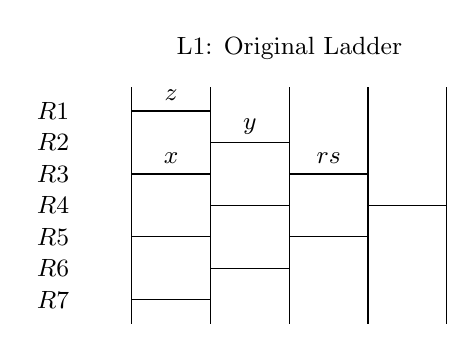
\begin{tikzpicture}
			\node at(2, 3.5){\small{L1: Original Ladder}};
			\draw(0, 0) to (0, 3);
					\node at(.5, 2.9){\small{$z$}};
				\draw(0, 2.7) to (1,2.7);
					\node at(.5, 2.1){\small{$x$}};

				\draw(0,1.9) to (1,1.9);
				\draw(0,1.1) to (1,1.1);
				\draw(0,0.3) to (1,0.3);
			\draw(1, 0) to (1, 3);
				\node at(1.5,2.5){\small{$y$}};
				\draw(1,2.3) to (2,2.3);
				\draw(1,1.5) to (2,1.5);
				\draw(1,0.7) to (2,0.7);
			\draw(2, 0) to (2, 3);
				\node at(2.5, 2.1){\small{$rs$}};
				\draw(2,1.9) to (3,1.9);
				\draw(2,1.1) to (3,1.1);
			\draw(3, 0) to (3, 3);
				\draw(3,1.5) to (4,1.5);
			\draw(4, 0) to (4, 3);

			\node at(-1, 2.7){\small{$R1$}};
			\node at(-1, 2.3){\small{$R2$}};
			\node at(-1, 1.9){\small{$R3$}};
			\node at(-1, 1.5){\small{$R4$}};
			\node at(-1, 1.1){\small{$R5$}};
			\node at(-1, .7){\small{$R6$}};
			\node at(-1, .3){\small{$R7$}};

			
		\end{tikzpicture}
	\end{minipage}
	\begin{minipage}{.4\textwidth}
		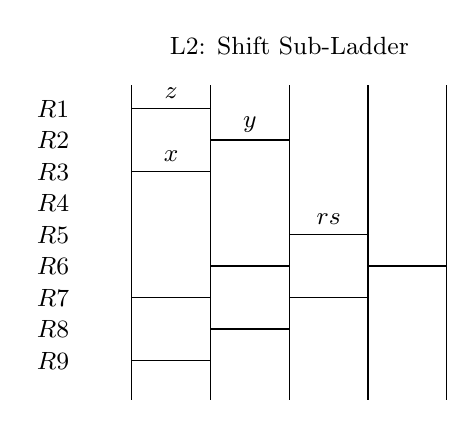
\begin{tikzpicture}
			\node at(2, 3.5){\small{L2: Shift Sub-Ladder}};

			\draw(0, -1) to (0, 3);
					\node at(.5, 2.9){\small{$z$}};
				\draw(0, 2.7) to (1,2.7);
					\node at(.5, 2.1){\small{$x$}};

				\draw(0,1.9) to (1,1.9);
				\draw(0,.3) to (1,.3);
				\draw(0,-0.5) to (1,-0.5);
			\draw(1, -1) to (1, 3);
				\node at(1.5,2.5){\small{$y$}};
				\draw(1,2.3) to (2,2.3);
				\draw(1,0.7) to (2,0.7);
				\draw(1,-0.1) to (2,-0.1);
			\draw(2, -1) to (2, 3);
				\node at(2.5, 1.3){\small{$rs$}};
				\draw(2,1.1) to (3,1.1);
				\draw(2,.3) to (3,.3);
			\draw(3, -1) to (3, 3);
				\draw(3,.7) to (4,.7);
			\draw(4, -1) to (4, 3);

			\node at(-1, 2.7){\small{$R1$}};
			\node at(-1, 2.3){\small{$R2$}};
			\node at(-1, 1.9){\small{$R3$}};
			\node at(-1, 1.5){\small{$R4$}};
			\node at(-1, 1.1){\small{$R5$}};
			\node at(-1, .7){\small{$R6$}};
			\node at(-1, .3){\small{$R7$}};
			\node at(-1, -.1){\small{$R8$}};
			\node at(-1, -.5){\small{$R9$}};


			
		\end{tikzpicture}
	\end{minipage}
		\begin{minipage}{.4\textwidth}
		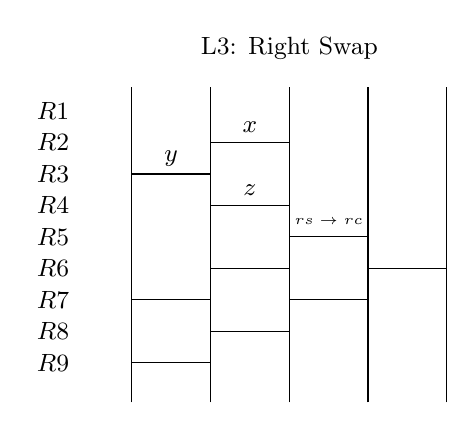
\begin{tikzpicture}
			\node at(2, 3.5){\small{L3: Right Swap}};

			\draw(0, -1) to (0, 3);
					\node at(1.5, 1.7){\small{$z$}};
				
					\node at(.5, 2.1){\small{$y$}};

				\draw(0,1.9) to (1,1.9);
				\draw(0,.3) to (1,.3);
				\draw(0,-0.5) to (1,-0.5);
			\draw(1, -1) to (1, 3);
				\node at(1.5,2.5){\small{$x$}};
				\draw(1,2.3) to (2,2.3);
				\draw(1, 1.5) to (2,1.5);
				\draw(1,0.7) to (2,0.7);
				\draw(1,-0.1) to (2,-0.1);
			\draw(2, -1) to (2, 3);
				\node at(2.5, 1.3){\tiny{$rs \rightarrow rc$}};
				\draw(2,1.1) to (3,1.1);
				\draw(2,.3) to (3,.3);
			\draw(3, -1) to (3, 3);
				\draw(3,.7) to (4,.7);
			\draw(4, -1) to (4, 3);

			\node at(-1, 2.7){\small{$R1$}};
			\node at(-1, 2.3){\small{$R2$}};
			\node at(-1, 1.9){\small{$R3$}};
			\node at(-1, 1.5){\small{$R4$}};
			\node at(-1, 1.1){\small{$R5$}};
			\node at(-1, .7){\small{$R6$}};
			\node at(-1, .3){\small{$R7$}};
			\node at(-1, -.1){\small{$R8$}};
			\node at(-1, -.5){\small{$R9$}};


			
		\end{tikzpicture}
	\end{minipage}
	\caption{$x,y,z$ to be right swapped. $rs$ is the right sibling; the root bar of the right sub-ladder.
	Going right to left, top to bottom. L1=original ladder, L2=shifting the right sub-ladder down two rows. L3 = right swap on $x,y,z$}
	\label{Fig:SwapAndShift}
\end{figure}

When a right swap operation is about to occur, bar $z$ will be moved from its current row and column to its current row + $3$ 
and its current column $+1$. Once the right swap opeartion is performed, 
the right sibling/$rs$ of $x$ becomes the right child/$rc$ of $z$.
The left swap operation is simply the inverse function of the right swap operation. 
Therefore, one can derive the left swap operation and the shift required for left swapping by deriving them 
from the right swap operation and the shift required for the right swap operation.

\begin{lemma}
	Shifting the entire sub-tree beginning at $rs$ down 
two rows ensures that $rs$ becomes $rc(z)$ and the ladder maintains its structure.
\end{lemma}
\begin{proof}
	Assume $ladder$ is a $1$ indexed two dimensional array. Going down the ladder is moving in the positive 
	direction and going up the ladder is moving in a negative direction. 
	Let $k$ be the current row of $z$. Let $k'=k+3$ be the target row of $z$. Let $m$ be the row of $rs$.
	We know that $m$ also equals the row of $x$ seeing as $rs$ is on the same row as $x$ prior to the 
	right swap operation. We know that $k$ = $m-2$ seeing as $z$ is two rows above $x$. Thus, 
	$k'=k+3=(m-2)+3=(m+1)$. Thus, the target row of $z=m+1$. Let $o$ be the current column of $z$.
	Let $o+1$ be the target column of $z$. We know that $o$ is 
	also the column of $x$ seeing as $z$ and $x$ are in the same column. 
	Thus, we know that the column of $rs$ is $o+2$ seeing as $rs$ is the right sibling  
	of $x$. Therefore the target destination of $z$ is $ladder[k'=m+1][o+1]$. 
	$rs$ is in the column $o+2$ and is at $row=m$ prior to the right swap opeartion. 
	We know that $rs \rightarrow rc(z)$ after the right swap operation, therefore $rs$ 
	must appear in the ladder at row $k'+1=m+1+1$ and the column of $o'+1$; please refer to theorem \ref{Theorem:One}
	for the definition of the right child. Since the column of $rs=o'+1$, then the column does not have to be changed.
	Since the current row of $rs$ is $m$, then the right sub-ladder needs to be shfited down by $+2$ to ensure 
	that $rs \rightarrow rc(z)$ after the right swap operation is performed. Since $rs$ also has right and left children, 
	each of them need to be shifted down two rows to ensure the ladder mainatins its structure whence the right swap 
	operation is performed. QED. 

\end{proof}


\pagebreak

%%input revoiew of second paper


\section{Ladder Lottery Realization}

In \emph{Ladder Lottery Realization}~\cite{A3}, written by Horiyama, Uno, Wasa and Yamanaka, the authors provide 
a rather interesting puzzle in regards to ladder lotteries. The puzzle 
is known as the Ladder Lottery Realization Problem. In order to understand
the problem, one must know what a \emph{multi-set} is. A \emph{multi-set}
is a set in which an element may appear more than once. The exponent 
above the element indicates the number of times it appears in the set.
For example, given the following multi-set, $\{3^{2}, 2^{4}, 5^{1}\}$ 
the element $3$ appears twice in the set, the element $2$ appears four times
in the set and the element $5$ appears once in the set.
The Ladder Lottery Realization puzzle asks, given an arbitrary starting permutation, $\pi$, 
and a multi-set of bars, 
is there a ladder lottery for $\pi$
that uses every bar in the multi-set the number 
of times it appears in the  multi-set. 
For an example of an affirmative solution to the Ladder Lottery Realization problem, see Figure~\ref{fig:ladder realization}.

\begin{figure}[!htp]
    \begin{center}
        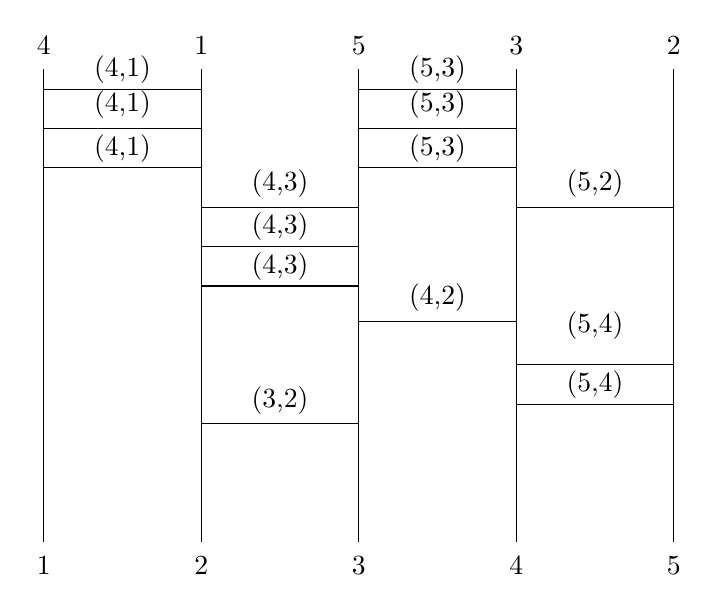
\begin{tikzpicture}
            \draw (0, 0) to (0, 6);
                \node at(0, -0.3){1};
                \node at(0, 6.3){4};
            \draw(2, 0) to (2, 6);
                \node at(2, -0.3){2};
                \node at(2, 6.3){1};
            \draw(4, 0) to (4, 6);
                \node at(4, 6.3){5};
                \node at(4, -0.3){3};
            \draw(6, 0) to (6, 6);
                \node at(6, 6.3){3};
                \node at(6, -0.3){4};
            \draw(8, 0) to (8, 6);
                \node at(8, 6.3){2};
                \node at(8, -0.3){5};

            %%draw the bars
                \node at(1, 6){(4,1)};
                    \draw(0, 5.75) to (2, 5.75);
            \draw(0, 5.25) to (2, 5.25);
                \node at(1, 5.55){(4,1)};
            \draw(0, 4.75) to (2, 4.75);
                \node at(1, 5){(4,1)};

            \draw(4, 5.75) to (6, 5.75);
                \node at(5, 6){(5,3)};
            \draw(4, 5.25) to (6, 5.25);
                \node at(5, 5.55){(5,3)};
            \draw(4, 4.75) to (6, 4.75);
                \node at(5, 5){(5,3)};

            \draw(2, 4.25) to (4, 4.25);
                \node at (3, 4.55){(4,3)};
            \draw(2, 3.75) to (4, 3.75);
                \node at (3, 4){(4,3)};
            \draw(2, 3.25) to (4, 3.25);
                \node at (3, 3.5){(4,3)};
            
            \draw(2, 1.5) to (4, 1.5);
                \node at(3, 1.8){(3,2)};
            
            \draw(4, 2.8) to (6, 2.8);
                \node at (5, 3.1){(4,2)};
            \draw(6, 4.25) to (8, 4.25);
                \node at (7, 4.55){(5,2)};
            
            \draw(6, 2.25) to (8, 2.25);
                \node at (7,2.75){(5,4)};
            
            \draw(6, 1.75) to (8, 1.75);
                \node at (7, 2){(5,4)};
            
        \end{tikzpicture}
    \end{center}
      


    \caption{An affirmative solution to the Ladder Lottery Realization Problem given a starting permutation $(4,1,5,3,2)$ and the multi set of bars $\{(3,2)^{1},(4,1)^{3}, (4,2)^{1},(4,3)^{3},(5,2)^{1},(5,3)^{3},(5,4)^{2}\}$}
    \label{fig:ladder realization}
\end{figure}
\pagebreak
The authors prove that the Ladder Lottery Realization problem in NP-Hard
by reducing the Ladder Lottery Realization to the One-In-Three 3SAT problem, 
which has already been proven to be NP-Hard.
The authors note that there are two cases in which the ladder lottery
realization problem can be solved in polynomial time. These cases 
include the following. First, if every bar in the multi-set appears
exactly once and every bar corresponds to an inversion, 
then an affirmative solution to the Ladder Lottery Realization 
instance can be achieved in polynomial time. 
Second, if there is an inversion in the permutation and its bar appears in the multi-set an even 
number of times, then a negative solution to
the Ladder Lottery Realization instance
can be achieved in polynomial time. This is because the elements that cross the bar will 
be uninverted when then be inverted again. Therefore $\pi$ will not be sorted by the ladder.\par

%%input review of third paper

\section{Optimal Reconfiguration of Optimal Ladder Lotteries}
In Optimal Reconfiguration of Optimal Ladder Lotteries, written by Horiyama, Wasa and Yamanaka,
the authors provide a polynomial solution to the 
\emph{minimal reconfiguration problem} which states that given 
two ladder is $OptL\{\pi\}$, $L_{i}$ and  $L_{m}$, what is the minimal number of 
swap operations to perform that will transition from $L_{i}$ to $L_{m}$~\cite{A2}?
The authors answer the question based on the local swap operations previously 
explained along with some other concepts. The first of these concepts 
is termed the \emph{reverse triple}~\cite{A2}. Basically, a reverse triple is a relation
between three bars, $x,y,z$ in two arbitrary ladders, $L_{i}, L_{m}$, such that if $x,y,x$
are right swapped in $L_{i}$, then they are left swapped in $L_{m}$ or if they are 
left swapped in $L_{i}$ then they are right swapped in $L_{m}$~\cite{A2}. 
The second of the concepts is the \emph{improving triple}~\cite{A2}. The improving triple is 
performing a right/left swapping three bars, $x,y,z$, in $L_{i}$ such that the 
result of the swap removes a reverse triple between
ladders $L_{i}$ and $L_{m}$~\cite{A2}. The improving triple is a symmetric 
relation, therefore performing a right/left swapping of the $x,y,z$ in $L_{m}$ also results in the 
removal of a reverse triple between $L_{i}$ and $L_{m}$~\cite{A2}.\par
The \emph{minimal length reconfiguration sequence} is the minimal number of 
improving triples required to transition from $L_{i}$ to $L_{m}$ or 
$L_{m}$ to $L_{i}$~\cite{A2}. Transitioning from $L_{i}$ to $L_{m}$ with the minimal length reconfiguration sequence 
is achieved by applying an improving triple to each of the reverse triples between 
$L_{i}$ and $L_{m}$. That is to say, the length of the reconfiguration sequence 
is equal to the number of improving triples required to remove all reverse triples between $L_{i}$ and  $L_{m}$~\cite{A2}.\par
The second contribution of this paper is that it provides a closed form formula for the 
upper bound for the minimal length reconfiguration sequence for any permutation 
of size $n$~\cite{A2}. That is to say, given some arbitrary $\pi$ of order $n$, what is the maximum 
length of the minimal length reconfiguration sequence between two ladders in $OptL\{\pi\}$?
The authors prove that there are two unique ladders in $OptL\{\pi=(n, n-1, \dots, 1)\}$ that 
have the upper bound for the minimal length reconfiguration sequence~\cite{A2}. These ladders are the root ladder and \emph{terminating ladder} in 
$OptL\{\pi=(n, n-1, \dots, 1)\}$ that have a minimal reconfiguration sequence equal to 
the upper bound. The terminating ladder in $OptL\{\pi=(n, n-1, \dots, 1)\}$ is defined as the ladder 
such that every possible right swap operation has been performed. The length of the reconfiguration sequence 
between the root ladder and terminating ladder in $OptL\{\pi=(n, n-1, \dots, 1)\}$ is $n{(n-1)~\choose 2}$~\cite{A2}. 
This is because the number of reverse triples between the root ladder and the terminating ladder 
in $OptL\{\pi(n, n-1, \dots, 1)\}$ is equal to $n{(n-1)~\choose 2}$. Thus, in 
order to reconfigure the root to the terminating ladder, or vice versa, each 
reverse triple between them must be improved by applying one improving triple.
\par

%%input review of fourth paper.

\section{Efficient Enumeration of all Ladder Lotteries with K Bars}

In this paper, the authors apply the same algorithm used in Efficient Enumeration of Optimal Ladder-Lotteries 
and its Application for generating all ladder lotteries with k bars. The number of elements 
in The inversion set of $\pi$ also known as $Inv\{\pi\}$ provides the lower bound for $K$ 
and the upper bound is positive infinity. Therefore $K=[|Inv\{\pi\}| \dots N]$\par\par 
\subsection{Coding Latter Lotteries}
\subsubsection{Overview}
In this paper, the authors provide three methods to encode ladder-lotteries as 
binary strings. Coding discrete objects as binary strings is an appealing theme because 
it allows for compact represntation of them for a computer \cite{A5}.
\subsubsection{Route Based Encoding}
The first method is termed \emph{route based encoding method} in 
which each route of an element in the permutation has a binary encoding. Let $L$
be a ladder-lottery for some arbitrary permutation $\pi$ of order $N$. The route 
of element $p_{i}$ is encoded by keeping in mind $p_{i}$ crosses bars in its route 
going left zero or more times and crosses bars in its route going right zero or 
more times \cite{A5}. The maximum number of bars $p_{i}$ can have is $N-1$, therefore the 
upper bound for the number of left/right crossings for $p_{i}$ is $N-1$ \cite{A5}. 
Let a left crossing be denoted with a $'0'$ and let a right crossing be denoted 
with a $'1'$. Let $C_{p_{i}}$ be the route encoding for the $i^{th}$ element 
in $\pi$. To construct $C_{p_{i}}$,  append $0$ and $1$ to each other representing 
the left and right crossings of $p_{i}$ from the top left 
to bottom right of the ladder \cite{A5}. If the number of crossings for $p_{i}$ 
is less than $n-1$, append $0s$ to the encoding of the route of $p_{i}$ until
the encoding is of length $N-1$ \cite{A5}. Let $LC_{L}$ be the route encoding for 
some arbitrary ladder in $OptL\{\pi\}$. $LC_{L}$ is $C_{p_{1}}, C_{p_{2}, \dots C_{p_{N}}}$.
For an example of the route encoding for the root ladder of $(3,2,5,4,1)$ refer to 
Fig.\ref{fig:route-encoding}. In \ref{fig:route-encoding}you will see that $C_{p_{1}}$ is 11\underline{00}. Underlined 
$0s$ are the $0s$ added to ensure the length of $C_{p_{1}}$ is $N-1$.
Since the length of $C_{pi}$ is $N-1$ and the number of elements in $\pi$ is $N$
then the length of $LC_{L}=N(N-1)$. Hence the number of bits needed for $LC_{L}$ 
belongs to $\mathcal{O}(N^{2})$.\par 
\begin{figure}[!htp]
    \begin{center}
        \begin{tikzpicture}
    
            %%draw the lines
            \draw(0, 0) to (0, 4);
                \node at(0, 4.3){3};
                \node at(0, -0.3){1};
            \draw(2, 0) to (2, 4);
                \node at (2, 4.3){2};
                \node at(2, -0.3){2};
            \draw(4, 0) to (4, 4);
                \node at (4, 4.3){5};
                \node at (4, -0.3){3};
            \draw(6, 0) to (6, 4);
                \node at (6, 4.3){4};
                \node at (6, -0.3){4};
            \draw(8, 0) to (8, 4);
                \node at (8, 4.3){1};
                \node at (8, -0.3){5};
    
            %%Draw the bars
            \draw(0, 2) to (2, 2);
            \draw(2, 1.5) to (4,1.5);
            \draw(0, 1) to (2, 1);

            \draw(4, 3) to (6, 3);
            \draw(6, 2.5) to (8, 2.5);
            \draw(4, 2) to (6, 2);
        \end{tikzpicture}
    \end{center}
   
 \caption{The route encoding for the following ladder lottery is 11\underline{00}01\underline{00}11\underline{00}01\underline{00}0000}
 \label{fig:route-encoding}

\end{figure}

\subsubsection{Line Based Encoding}
The second method is termed \emph{line based encoding} which focuses 
on encoding the lines of the ladder-lottery. Each line is represented 
as a sequence of endpoints of bars. Let $L$ be an optimal ladder-lottery 
with $N$ lines and $B$ bars, then for some arbitrary line, $i$, there 
are zero or more right/left endpoints of bars that 
come into contact with $i$ \cite{A5}. Let $LC_{i}$ denote the line based encoding for line $i$.
Let $1$ denote a left end point that 
comes into contact with line $i$ and let $0$ denote a right 
end point that comes into contact with line $i$. Finally, append a $0$
to line $i$ to denote the end of the line. Then line $i$ can be 
encoded, from top to bottom, as a sequence of $1s$ and $0s$ that 
terminates in a $0$.  Given the ladder in Fig. \ref{fig:line-encoding}, 
$LC_{3}$ is $001\underline{0}$. The \underline{0} denotes 
the end of the line. Let $LC_{L}$ be the line encoding for 
some arbitrary ladder, then $LC_{L}=LC_{1}, LC_{2}, \dots LC_{N}$.
Let $L_{(4,2,3,1)}$ refer to the ladder in Fig. \ref{fig:line-encoding}, then 
$LC_{L_{(4,2,3,1)}}=11\underline{0}010\underline{0}110\underline{0}010\underline{0}0\underline{0}$\par 
In order to reconstruct $L$ from its $LC_{L}$, or in other words decode
$LC_{L}$ it is important to recognize that the first line only has left endpoints attached to it
\cite{A5}. Since left end points are encoded as a $1$ then it is guarenteed that the first $0$ 
represents the end of line $1$. Secondly, the last/$Nth$ line 
has only right end points attached to it.  Therefore $LC_{N}$ will only have $0s$. Therefore, $LC_{N}$
does not require a terminating $0$. Thirdly, for any 
line $i+1$, if line $i+1$ has a $0$ then there must be a corresponding $1$
in line $i$. That is to say, if the right end point of a bar is on line 
$i+1$ then that same bar must have a left endpoint on line $i$. To decode 
$LC_{L}$ start by decoding line $1$. The line will contain $0$ or more 
left end points. To decode $LC_{i+1}$ where $i+1>1$, go to 
$LC_{i}$ and match each $1$ in $LC_{i}$ with a $0$ in $LC_{i+1}$. 
Let $k=$ the number of $1s$ in $LC_{i}$. Let $j=$ the number 
of $0s$ in $LC_{i+1}$ then $k=j-1$; due to the last $0$ in $LC_{i+1}$ denoting 
the end of line $i+1$.  Intuitively, this means match every left end point 
of a bar in line $i$ with a right end point in line $i+1$. The last $0$
represents the end of line $i+1$. For an example of a full decoding of $LC_{L_{(4,2,3,1)}}$
please refer to Fig. \ref{fig:line-encoding}.\pagebreak
\begin{figure}[!htp]
    \begin{center}
        \begin{tikzpicture}
            \draw(0, 0) to (0, 4);
            \node at (0, 4.3){4};
            \node at (0, -0.3){1};
        \draw(2, 0) to (2, 4);
            \node at (2, 4.3){2};
            \node at (2, -0.3){2};
        \draw(4, 0) to (4, 4);
            \node at (4, 4.3){3};
            \node at (4, -0.3){3};
        \draw(6, 0) to (6, 4);
            \node at (6, 4.3){1};
            \node at (6, -0.3){4};

        %%bars 
        \draw(0, 3) to (0.7, 3);
            \node at (0.35, 3.3){1};
        \draw (1.3, 3) to (2, 3);
            \node at (1.65, 3.3){0};

        \draw(2, 2.5) to (2.7, 2.5);
            \node at (2.35, 2.8){1};
        \draw(3.3, 2.5) to (4, 2.5);
            \node at (3.65, 2.8){0};

        \draw(4, 2) to (4.7, 2);
            \node at (4.35, 2.3){1};
        \draw(5.3, 2) to (6, 2);
            \node at (5.65, 2.3){0};

      

        \draw(2, 1) to (2.7, 1);
            \node at (2.35, 1.3){1};
        \draw(3.3, 1) to (4, 1);
            \node at (3.65, 1.3){0};

        \draw(0, 0.5) to (0.7, 0.5);
            \node at (0.35, 0.8){1};
        \draw(1.3, 0.5) to (2, 0.5);
            \node at (1.65, 0.8){0};

        \end{tikzpicture}
      

    \end{center}
    \caption{$LC_{L(4,2,3,1)}=LC_{1}=11\underline{0},LC_{2}=0110\underline{0},LC_{3}=010\underline{0},LC_{4}=0$}
    \label{fig:line-encoding}
\end{figure}

Since each bar is encoded as two bits, and there are $N-1$ bits as terminating bits; 
one for each line in $L$, then the number of bits required is $N + 2B -1$, where $N$
is the number of lines and $B$ is the number of bars. Encoding and decoding can be 
done in $\mathcal{O}(n+b)$ time.\cite{A5} Clearly the line-based encoding 
trumps the route-based encoding in both time and space complexity.

\subsubsection{Improved Line-Based Encoding}
Although the line-based encoding is better than the route based 
encoding, it can still be further optimized. The authors provide 
three improvements to the line-based encoding. These three improvements
can be combined to really help imrpove the line based encoding's 
space efficiency \cite{A5}. 
\paragraph{Imrpovement 1}
Since the $Nth$ line has only right endpoints attached to it, 
then it actually does not need to be encoded. Right endpoints 
are denoted as $0$ and left endpoints are encoded as $1$, therefore the number of right endpoints 
for line $N$ is equal to the number of $1s$ in $LC_{N-1}$.
Thus, there is no need for $LC_{N}$ \cite{A5}. The encoding with improvment 
one for the ladder in Fig. \ref{fig:line-encoding} is $11\underline{0}0110\underline{0}010$.
\paragraph{Improvement 2}
Improvement two is based off of the fact that for any two bars,
$x,y$, let $l_{x}$ denote the left endpoint of bar $x$, let 
$l_{y}$ denote the left endoint of bar $y$, let $r_{x}$ denote 
the right end point of bar $x$ and let $r_{y}$ denote the right 
end point of bar $y$. Let line $i$ be the line of $l_{x}$ and $l_{y}$
and let line $i+1$ be the line of $r_{x}$ and $r_{y}$.
\begin{lemma}
There are three possible cases for the 
placement of $x$ and $y$ in some 
arbitrary ladder from $OptL\{\pi\}$. The first case is that there 
is at least one other bar, $z$, with a right end point, $r_{z}$ between $l_{x}$
and $l_{y}$ on line $i$. The second case is that there is at least one other bar 
$z$, with a left end point, $l_{z}$, between $r_{x}$ and $r_{y}$ on line $i+1$. 
The third case is that there is at least one bar, $z$, with a right end point, 
$r_{z}$, betwen $l_{x}$ and $l_{y}$ on line $i$ and there is at least one other bar, 
$z\prime$ with a left end point, $l_{z\prime}$, between $r_{x}$ and $r_{y}$ on line $i+1$ \cite{A5}. 
For an example of all three cases refer to Fig. \ref{fig:three-cases}\par
\end{lemma}

%%figure demonstrating the three cases for bar positions
\begin{figure}[!htp]
       
            %%first case
            \begin{minipage}{.3\textwidth}
                \begin{tikzpicture}
                    \draw(0, 0) to (0, 4);
                        \node at (2, 4.3){\small{$i+1$}};
                    \draw(1, 0) to (1, 4);
                        \node at (1, 4.3){\small{$i$}};
                    \draw(2, 0) to (2, 4);
                        \node at (0, 4.3){\small{$i-1$}};
                    \draw(0, 2) to (1, 2);
                        \node at (.5, 2.3){\small{$r_{z}$}};
                    \draw(1, 3) to (2, 3);
                        \node at (1.5, 3.3){\small{$l_{x}$}};
                    \draw(1, 1) to (2, 1);
                        \node at (1.5, 1.3){\small{$l_{y}$}};
                \end{tikzpicture}
            \end{minipage}
              \begin{minipage}{.3\textwidth}

                 \begin{tikzpicture}
                
                  \draw(0, 0) to (0, 4);
                     \node at (0, 4.3){\small{$i-1$}};
                  \draw(1, 0) to (1, 4);
                    \node at (1, 4.3){\small{$i$}};
                  \draw(2, 0) to (2, 4);
                     \node at (2, 4.3){\small{$i+1$}};
                   \draw(0, 3) to (1, 3);
                         \node at (.5, 3.3){\small{$r_{x}$}};
                    \draw(1, 2) to (2, 2);
                         \node at (1.5, 2.3){\small{$l_{z}$}};
                     \draw(0, 1) to (1, 1);
                         \node at (0.5, 1.3){\small{$r_{y}$}};
                
                   
                
                \end{tikzpicture}
             \end{minipage}
             \begin{minipage}{.3\textwidth}

                \begin{tikzpicture}
                
                 \draw(0, 0) to (0, 4);
                    \node at (1, 4.3){\small{$i$}};
                 \draw(1, 0) to (1, 4);
                    \node at (2, 4.3){\small{$i+1$}};
                 \draw(2, 0) to (2, 4);
                    \node at (0, 4.3){\small{$i-1$}};
                 \draw(3, 0) to (3, 4);
                    \node at (3, 4.3){\small{$i+2$}};
                    \draw(1, 3) to (2, 3);
                        \node at (1.3, 3.3){\small{$l_{x}$}};
                        \node at (1.7, 3.3){\small{$r_{x}$}};
                     \draw(0, 2) to (1, 2);
                        \node at (0.7, 2.3){\small{$r_{z}$}};
                    \draw(1, 1) to (2, 1);
                        \node at (1.3, 1.3){\small{$l_{y}$}};
                         \node at (1.7, 1.3){\small{$r_{y}$}};
                     \draw(2, 2) to (3, 2);
                        \node at (2.3, 2.3){\small{$l_{z\prime}$}};
                
                   
                
                \end{tikzpicture}
            \end{minipage}
        

    \caption{Three examples of the three cases for the placement 
    of bars $x$ and $y$ in a ladder-lottery}
    \label{fig:three-cases}
\end{figure}
\begin{proof}
    Suppose that none of the above cases hold. Let $L_{\pi}$ be an 
    optimal ladder-lottery with bars $x$ and 
    bar $y$. If none of the cases hold then $x$ and $y$ are directly above/below each other without 
    the enpoint of some third bar $z$ between $l_{x}$ and $l_{y}$ or between $r_{x}$ and $r_{y}$.
    Let $x$ be the bar for the inversion of two elements $p$ and $q$ in $\pi$. 
    As $p$ and $q$ travel through the ladder they will cross each other at bar $x$; 
    thus uninverting them. Since bar $y$ is directly below bar $x$, then $p$ and $q$ will cross 
    bar $y$ thus re-inverting them. Therefore, there will need to be a third 
    bar that uninverts $p$ and $q$ a second time. Since this third bar is 
    redundant, $L_{\pi}$ is non-optimal which is a contradiction. Let $x$ be a bar for two 
    elements in $\pi$, $p$ and $q$ such that $p$ and $q$ do not form an inversion. Then $x$ 
    will invert $p$ and $q$ and $y$ will uninvert them. Thus making both $x$ and $y$ redundant
    bars which is also a contradiction. Therefore one of the above cases must hold.
\end{proof}
Knowing that one of the three above cases must hold is beneficial for improving the 
line-based encoding. If $l_{x}$ and $l_{y}$ on line $i$ have no $r_{z}$ between them, 
then there must be at least one $l_{z\prime}$ between $r_{x}$ and $r_{y}$ on line $i+1$.
Since a left endpoint is encoded as a $1$ and a right endpoint is encoded as a $0$, 
a $1$ can be omitted for the encoding of line $i+1$ if $l_{x}$ and $l_{y}$ have no $r_{z}$
between them on line $i$ \cite{A5}. That is to say, if there is not a $0$ between 
the two  $1s$ for $l_{x}$, $l_{y}$ in $LC_{i}$, it is implied that there is at least one $1$ between 
the two $0s$ for $r_{x}$, $r_{y}$ on $LC_{i+1}$. Hence, one of the $1s$ in $LC_{i+1}$ can be omitted. 
The line encoding with improvement two for the ladder in Fig. \ref{fig:line-encoding} is $11\underline{0}010\underline{0}00\underline{0}0$.
\paragraph{Imrpovement 3}
Improvement three is based off of saving some bits for right 
end points/$0s$ in $LC_{N-1}$. Since line $N$ has no left end points,
then then there must be some right endpoints between any two 
consecutive bars connecting lines $N-1$ and line $N$. If you 
refer to Fig. \ref{fig:improvement3}, then the only configuration for lines $N-2, N-1, N$
is the middle configuration \cite{A5}. Knowing this, then 
given two bars, $x$ and $y$ with $l_{x}$/$l_{y}$ on line 
$n-1$ and $r_{x}$/$r_{y}$ on line $n$, there must be at least 
one bar, $z$, with its $r_{z}$ between $l_{x}$ and $l_{y}$
on line $N-1$. Thus, for every $1$ in $LC_{N-1}$ except the 
last $1$ in $LC_{N-1}$, a $0$ must immidediately proceed any $1$
in $LC_{N-1}$. Since this $0$ is implied, it can be removed from $LC_{N-1}$ \cite{A5}. 
For an example of improvement three with its line encoding for $LC_{N-1}$ please refer to Fig.\ref{fig:improvement3}\pagebreak
\begin{figure}[!htp]
    \centering
    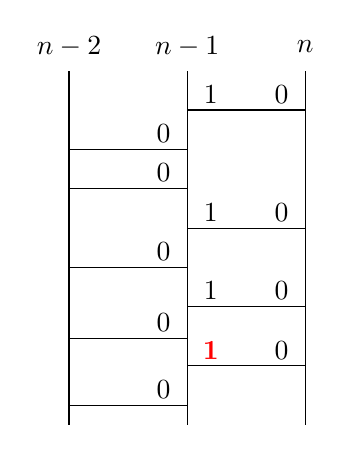
\begin{tikzpicture}
        \draw(0, -0.5) to (0, 4);
            \node at (0, 4.3){$n-2$};
            \draw(0, 3) to (1.5, 3);
                \node at (1.2, 3.2){$0$};
            \draw(0, 2.5) to (1.5, 2.5);
                \node at (1.2, 2.7){$0$};
            \draw(0, 1.5) to (1.5, 1.5);
                \node at (1.2, 1.7){$0$};
            \draw(0, 0.6) to (1.5, 0.6);
                 \node at (1.2, 0.8){$0$};
            \draw(0, -0.25) to (1.5, -0.25);
                \node at (1.2, -0.05){$0$};
        \draw(1.5, -0.5) to (1.5, 4);
            \node at (1.5, 4.3){$n-1$};
            \draw(1.5, 3.5) to (3, 3.5);
                \node at (1.8, 3.7){$1$};
                \node at (2.7, 3.7){$0$};
            \draw(1.5, 2) to (3, 2);
                \node at (1.8, 2.2){$1$};
                \node at (2.7, 2.2){$0$};
            \draw(1.5, 1) to (3, 1);
                \node at (1.8, 1.2){$1$};
                \node at (2.7, 1.2){$0$};
            \draw(1.5, 0.25) to (3, 0.25);
                \node at (1.8, 0.45){$\textcolor{red}{\textbf{1}}$};
                \node at (2.7, 0.45){$0$};

        \draw(3, -0.5) to (3, 4);
            \node at (3, 4.3){$n$};
    \end{tikzpicture}
    \caption{The line coding for $LC_{N-1}$ with imrpovement three is $101110$\underline{$0$}. The red, bold $1$ represents 
    the last left end point in $LC_{N-1}$, therefore the proceeding $0$ must be 
    included in $LC_{N-1}$. For every other $1$ in $LC_{N-1}$, a $0$ is omitted following 
    said $1$.}
    \label{fig:improvement3}
\end{figure}
\paragraph{Combining All Three}
The combination of all three improvements can be done independently. 
Let $IC_{L_{(4,2,3,1)}}$ be the \emph{improved line-based encoding} for $L_{(4,2,3,1)}$ 
by applying improvements 1-3 to $LC_{L_{(4,2,3,1)}}$. Recall that $LC_{L}$ denotes the line-based encoding for some ladder $L$.
$LC_{L_{(4,2,3,1)}}$ for the ladder in Fig. \ref{fig:line-encoding} is $11\underline{0}10101\underline{0}0010101\underline{0}000$.
By applying imrpovement one, we get $11\underline{0}101011\underline{0}0010101\underline{0}$. 
Notice how the last three $0s$ from $LC_{L}$ were removed because they represented $LC_{N}$.
By applying imrpovement two to improvememt one we get $11\underline{0}10011\underline{0}001001\underline{0}$.
Notice how the second, and eigth $1$ were removed because they are implied by 
the successive $0s$. By applying improvement three to the result of improvement 
two we get $11\underline{0}10011\underline{0}00101\underline{0}$. Notice how the last $0$ 
was removed from improvement two. This is because the $0$ is implied in $LC_{N-1}$
due to the configuration between of bars connecting lines $N-1$ and line $N$. The $IC_{L_{(4,2,3,1)}}$ for the ladder in fig. \ref{Fig:allthree} 
is $IC_{L_{(4,2,3,1)}}=11\underline{0}10011\underline{0}00101\underline{0}$.\pagebreak

\begin{figure}[!htp]
     \centering
    \begin{tikzpicture}
         \draw(0, 0) to (0, 4);
             \node at (0, 4.3){$n-3$};
             \draw(0, 3.5) to (1.5, 3.5);
             \draw(0, 2.5) to (1.5, 2.5);
         \draw(1.5, 0) to (1.5, 4);
             \node at (1.5, 4.3){$n-2$};
             \draw(1.5, 3) to (3, 3);
             \draw(1.5, 3.8) to (3, 3.8);
             \draw(1.5, 2) to (3, 2);
             \draw(1.5, 1) to (3, 1);
         \draw(3, 0) to (3, 4);
             \node at(3, 4.3){$n-1$};
             \draw(3, 2.5) to (4.5, 2.5);
             \draw(3, 1.5) to (4.5, 1.5);
             \draw(3, 0.5) to (4.5, 0.5);
         \draw(4.5, 0) to (4.5, 4);
             \node at(4.5, 4.3){$n$};
     \end{tikzpicture}
     \caption{A ladder used to illustrate all three improvements $IC_{L}$. $IC_{L}=11\underline{0}10011\underline{0}00101\underline{0}$}
     \label{Fig:allthree}
\end{figure}

%%%section on how ladde lotteries relate to other mathematical objects
% Despite the fact that ladder lotteries have only been stuidied in and
% of themseleves for ten years, they are closely tied to other mathematical 
% phenomena that have been studied for much longer. These mathematical phenomena  
%  include \emph{Pseudo Lines} which are an arrangement of 
% curves on a plane such that given two curves, they only intersect 
% at most once and at each intersection, only two curves intersect.See figure --reference--
% for a wiring diagrams of the pseudo line arrangement for the 
% permutation, $(5,4,3,2,1)$. The other mathematical phenomena is \emph{adjacent transpositions}
% which is a swap of two adjacent elements in a permutation. 
\subsection{Ladders and Adjacent Transpositions}
A ladder lottery is a way of sorting a permutation, yet it can also be thought of as 
a decomposition of a permutation into \emph{adjacent transpositions}. \cite{A1} 
An \emph{adjacent transposition} is simply a swap of two adjacent elements in a 
permutation. For example, given the permutation (1, 3, 4, 2), an adjacent 
transposition could be done on the following pairs of elements: 
(1, 3), (3, 4) or (4, 2). Each would result in a unique permutation. 
Simply put, given any arbitrary starting permutation, $\pi$, keep swapping 
adjacent inversions until the identity permutation is reached.  An optimal 
ladder lottery from $\pi's$ optimal ladder set is a minimal sequence of 
adjacent transpositions such that $\pi$ is sorted into the identity permutation; 
each ladder in the set represents a sequence of adjacent transpositions for 
sorting $\pi$ into the identity permutation. For example, given the permutation 
(4, 3, 2, 1) there exists eight ladders in this permutation's optimal ladder set. 
Two of these ladders are found in \ref{fig:ac}:

\begin{figure}[!htp]
    \label{fig:ac}
	\begin{minipage}{0.4\textwidth}
		\centering
	
		\begin{tikzpicture}
			\draw(0, 0) to (0, 4) node[above]{4};
			\draw(2, 0) to (2, 4) node[above]{3};
			\draw(4, 0) to (4, 4) node[above]{2};
			\draw(6, 0) to (6, 4) node[above]{1};
			
			\draw(0, 3.7) to (2, 3.7);
				\draw node at (1, 3.9) {(4, 3)};
			\draw(2, 3.25) to (4, 3.25);
				\draw node at (3, 3.45){(4, 2)};
			\draw(4, 2.75) to (6, 2.75);
				\draw node at (5, 3.0){(4, 1)};
			
			\draw(0, 2.75) to (2, 2.75);
				\draw node at (1, 3.0){(3, 2)};
			\draw(2, 2.25) to (4, 2.25);
				\draw node at (3, 2.5){(3, 1)};
			
			
			\draw(0, 1.75) to (2, 1.75);
				\draw node at (1, 1.95){(2, 1)};
			
			\draw node at (0, -0.5){1};
			\draw node at (2, -0.5){2};
			\draw node at (4, -0.5){3};
			\draw node at (6, -0.5){4};
			
			%%second ladder%%
			\draw(9, 0) to (9, 4) node[above]{4};
			\draw(11, 0) to (11, 4)node[above]{3};
			\draw(13, 0) to (13, 4)node[above]{2};
			\draw(15, 0) to (15, 4)node[above]{1};
			
			\draw(9, 3.7) to (11, 3.7);
				\draw node at (10, 3.9) {(4, 3)};
			\draw(11, 3.25) to (13, 3.25);
				\draw node at (12, 3.45){(4, 2)};
			\draw(13, 2.75) to (15, 2.75);
				\draw node at (14, 3.0){(4, 1)};
			
			\draw(9, 1.25) to (11, 1.25);
				\draw node at (10, 1.5){(3, 1)};
			\draw(11, 2) to (13, 2);
				\draw node at (12, 2.25){(2, 1)};
			
			\draw(11, 0.65) to (13, 0.65);
				\draw node at (12, 0.85){(3, 2)};
			 
			
			\draw node at (9, -0.5){1};
			\draw node at (11, -0.5){2};
			\draw node at (13, -0.5){3};
			\draw node at (15, -0.5){4};	
		\end{tikzpicture}
	
	\end{minipage}
	

	
		
	\caption{The left ladder is one of eight unique ladders from (4,3,2,1)'s optimal ladder set. The right ladder is another one of eight unique ladders form (4,3,2,1)'s optimal ladder set}
		
\end{figure}

From looking at the above ladders, going from top left to bottom right, the left ladder represents the sequence of adjacent transpositions (4,3), (4,2), (4,1),(3,2),(3,1),(2,1) 
whereas the right ladder represent the sequence of adjacent transpositions 
(4, 3),(4, 2),(4, 1),(2, 1),(3, 1),(3, 2). 
Notice how the length of the sequences are the same,because both lengths are equal 
to the minimal number of swaps to sort (4, 3, 2, 1) 
it is simply the order in which the adjacent transpositions occur in the sequence 
that makes the sequences different from each other. 

\chapter{The Counting Problem}
\label{chapter:countingProblem}
---Will Complete This Chapter Later---

%----------------  METHODOLOGY and IMPLEMENTATION ----------------------
\chapter{The Listing Problem}  
\label{chapter:listingproblem}
\subsection{Introduction to the Problem}
Listing problems are common problems in cambinatorics. In general, listing problems 
focus on enumerating the objects of a given finite set in some specific order. The listing problem in this thesis 
will be termed \emph{The Canonical Ladder Listing Problem}. The problem is stated as follows: Let $\pi_{N}$ be one of $N!$ arbitrary permutation of $[1 \dots N]$. 
Let \emph{The Canonical Ladder} be a unique ladder from $OptL\{\pi_{N}\}$. Let $CanL{\pi_{N}}$ be the set of all canonical ladders for 
all $N!$ permutations of order $N$. Let $L_{i}$ be the canonical ladder of some arbitrary permuation $OptL\{\pi_{N_{i}}\}$. A \emph{change} is defined as the insertion or 
deletion of one or more bar(s) to get from $L_{i}$ to $L{i+1}$, or the relocation of one or more bars in $L_{i}$ to get to $L_{i+1}$. The relocation of a bar 
is defined as moving a bar from a given row and column, to a new row and column in the ladder. The \emph{Listing Problem} asks given all permutations of 
order $N$, is there a way to generate the canonical ladder from each $OptL\{\pi_{N}\}$. 
Furthermore, if there is a way to do so, what is the most efficient way to do so. Efficiency is defined as 
using minimal change to transition from $L_{i}$ to $L_{i+1}$. For example, let $N=4$, there are $N!$ or 24 permutations 
of order $N$. $|CanL{\pi_{N}}=24|$; therefore there are 24 canonical ladders, one from each $OptL\{\pi_{4}\}$. Is there a way to generate 
all 24 canonical ladders for each $OptL\{\pi_{N}\}$? Furthermore, if there is such a way, what is the most efficient way 
to do so; i.e. the algorithm that requires the minimal amount of change to get from $L_{i}$ to $L_{i+1}$. See Table -- for 
the 24 permutations of order 4.
\begin{table}[]
    \begin{center}
       \begin{tabular}{|c |c |c |c |}
        \hline
        1234 & 1243 & 1324 & 1342 \\ \hline
        1423 & 1432 & 2143 & 2134 \\ \hline 
        2314 & 2341 & 2413 & 2431 \\ \hline 
        3124 & 3142 & 3214 & 3241 \\ \hline 
        3412 & 3421 & 4123 & 4132 \\ \hline 
        4213 & 4231 & 4312 & 4321 \\ \hline 
        
    \end{tabular}
    \caption{Table for all 4!, 24, permutations of order 4} 
    \end{center}

 \end{table}



Each of these permutations has one or more ladders in each of their respective 
$OptL\{\pi\}$. The canonical ladder listing  problem asks, given some arbitrary $N \geq 1$,
what is the most efficient way to list $CanL\{\pi_{N}\}$. Recall that in order to get from $L_{i}$ to $L_{i+1}$, at least one of the 
two changes must be applied to $L_{i}$ to get to $L_{i+1}$. At least one bar has to be removed/added or at least one bar 
has to be reolocated in $L_{i}$ to get to $L_{i+1}$.

\begin{theorem}
    In order to transition from canonical ladder $L_{i}$ to canonical ladder $L_{i+1}$, at least one bar has to be added or 
    removed from $L_{i}$ or at least one bar has to be relocated in $L_{i}$.
\end{theorem}
\begin{proof}
    We begin this proof by contradiction. Suppose $L_{i}$ is some arbitrary canonical ladder for permutation of 
    order $N$. Suppose that $L_{i+1}$ is the next canonical ladder in the set of canonical ladders. Each canonical 
    ladder represents a network of adjacent transposisitions of the corresponding permutations, $\pi_{i}$ and 
    $\pi_{i+1}$ used to sort $\pi_{i}$ and $\pi_{i+1}$ respectively. $\pi_{i}$ and $\pi_{i+1}$ are unique. Let $Inv{\pi}$ 
    be the set of all inversions is $\pi$. Let $AdjInv{\pi} \subset Inv{\pi}$ be a subset of inversions in $\pi$
    that are adjacent. A bar in $L_{i}$ and $L_{i+1}$ uninverts an adjacent inversion in from $AdjInv{\pi_{i}}$ and $AdjInv{\pi_{i+1}}$ respectively. 
    Note, that when an adjacent inversion is uninverted, a new intermediate permuation is derived from $\pi$. Let $IntPi(\pi)$
    be the permutation of intermediate permutations, beginning with $\pi$ that result from performing adjacent transpositions on $AdjInv{\pi}$, terminating with 
    the sorted permutation. The row in the ladder represents the order of uninverting adjacent transpositions in some intermediate permutation in $IntPi(\pi)$.
    For example, row 1 in $L_{i}$ represents uninverting adjacent inversions in $\pi_{i}$. The result of uninverting these 
    adjacent inversions is the second intermediate permutation in $IntPi(\pi)$, $\pi'$. Row two represents uninverting the adjecent 
    inversions in $\pi'$ resulting in $\pi''$, etc. If no bars are added or removed from $L_{i}$ then 
    the number of bars in $L_{i+1}$ is the same as in $L_{i}$. This means that the number of adjacent inversions that are uninverted 
    in $\pi_{i}$ is the same as in $\pi_{i+1}$. Next, suppose that no bars are relocated in $L_{i}$ to get to $L_{i+1}$. This would 
    mean that the same adjacent inversions in $\pi_{i}$ exist in $\pi_{i+1}$ and furthermore, the order in which these adjacent 
    iversions were uninverted would be the same for $\pi_{i}$ and $\pi_{i+1}$; in other words the $IntPi(\pi_{i})=IntPi(\pi_{i+1})$ But this is a contradiction, 
    seeing as $pi_{i}$ and $pi_{i+1}$ are unique. Therefore, at least one 
    bar has to be added or removed from $L_{i}$ to get to $L_{i+1}$ or at least one bar in $L_{i}$ has to be relocated to get to $L_{i+1}$.
    See fig- for an example of $L_{3 1 4 2}$ with the corresponding $IntPi(3 1 4 2)$.
\end{proof}

\begin{figure}[!htp]
    \begin{center}
    \begin{tikzpicture}
        %%draw the lines
        \draw(0, 0) to (0, 4);
            \node at(0, 4.3){3};
            \node at(0, -0.3){1};
        \draw(2, 0) to (2, 4);
            \node at(2, 4.3){1};
            \node at(2, -0.3){2};
        \draw(4, 0) to (4,4);
            \node at(4, 4.3){4};
            \node at(4, -0.3){3};
        \draw(6, 0) to (6, 4);
            \node at(6, 4.3){2};
            \node at(6, -0.3){4};
        \node at(8, 3){3,1,4,2};
        \node at(8, 2){1,3,2,4};
        

        \node at(-2, 4.3){$R_{0}$};
        \node at(-2, 3){$R_{1}$};
        \node at(-2, 2){$R_{2}$};
        \node at(-2, -0.3){$R_{3}$};

        %%draw the bars
        \draw(0, 3) to (2, 3);
        \draw(2, 2) to (4, 2);
        \draw(4, 3) to (6,3);

    \end{tikzpicture}
    \end{center}
    \caption{The rows are on the left of the ladder designating the order in which the adjacent inversions will be uninverted.
    On the right is the $IntPi(3,1,4,2)$ that results from the ladder univerting  the adjacent inversions in 3,1,4,2 in the order 
    of the rows. $IntPi(3,1,4,2)=((3,1,4,2), (1,3,2,4), (1,2,3,4))$}
\end{figure}

In this thesis, two listing algorithms were used to generate the canonical 
ladders for each $OptL\{\pi_{N}\}$. The first of these listing algorithms 
is a modification of the Steinhaus-Johnson-Trotter permutation listing algorithm. 
The second listing algorithm is, as far as I know, a novel algorithm. 
It is termed the cyclic-inversion algorithm. Both of these algorithms will 
be described, explained and analyzed throughout the remainder of the chapter.\par

Before proceeding, the justification for the canonical ladder will be presented. 
The canonical ladder is selected as the root ladder from each $OptL\{\pi_{N}\}$. 
The rationale for always choosing the root ladder was due to the fact that every 
permutation has a root ladder in its $OptL\{\pi\}$ whereas not every permutation 
has a non-root ladder. For example, given the permutation $(2,1,4,3)$, $OptL\{(2,1,4,3)\}$
has only one ladder which is the root ladder. This is because there are only two 
bars in the ladder, thus there is no swap operation that can be performed.
\begin{theorem}
    If $|OptL\{\pi\}|=1$ then the ladder is the root ladder.
\end{theorem} 
\begin{proof}
    The root ladder is defined as the ladder whose clean level is one.
    This means either there is no bar of a lesser element above the route a 
    greater element. Keeping in mind that the clean level of the root ladder is one, next consider what is meant by a  \emph{child bar}
     which is a bar to the bottom left or right of a given bar $x$. Within the context of the root ladder, 
     if the left endpoint of the child bar is directly below the right end point of $x$ then the child is a 
    right child of $x$. If the right end point of the child bar is directly 
    below the left end point of $x$ then it is a left child. 
    Keeping in mind the root ladder has not undergone any right swap operations, then
    if a child is a right child 
    then the child belongs to the same route of $x$ in the root ladder. 
    Let $R_{m}$ denote this route. Let $x$ be a bar representing an inversion with element $m$ and $k$.
    The right child of $x$ is a bar which represents an inversion 
    with $m$ and some element to the right of $k$. Suppose this was not the case, 
    then this would mean that the right child of $x$ was either a bar representing an inversion 
    between some element $m'$ that was greater than $m$ or lesser than $m$. If $m'$ was 
    greater than $m$ then this would be a contradiction seeing as $x$ would be above the bar of a route 
    of a greater element which contradicts the definition of the root ladder. On the other hand if 
    $m'$ were lesser than $m$, then $m$ would form an inversion with $m'$ and therefore 
    the bar representing this inversion would be part of the route of $m$ route. Thus, the right child 
    of a bar $x$ belongs to the same route as $x$ in the root ladder.\par The left child of $x$
    represents an inversion with some lesser element than $m$ and $k$. Suppose this was not the case, 
    then the left child could belong to a route greater than $m$, but if that were the case, this contradicts 
    the definition of the root ladder.
    Thus the first element of the left child must belong to the route of some lesser element than $m$. Next suppose that 
    the lesser element of the left child of $x$ was not $k$. Let this element be termed $k'$.
    $k'$ forms an inversion with the greater element of the left child of $x$. But since the greater element of the left child is less than $m$, 
    then $m$ would also form an inversion with $k'$. Thus, the bar of $m$ and $k'$ would be the parent of the left child, which is also 
    a contradiction, seeing as the left child is the child of bar $x$. Therefore the left child of $x$ must be a bar that 
    it belongs to the route of a lesser element than $m$ and its lesser element is $k$.\par 
    Please refer to FIG--- to view an example of a root ladder with left and right children.\pagebreak

    
\end{proof}


\begin{figure}[!htp]
    \begin{center}
    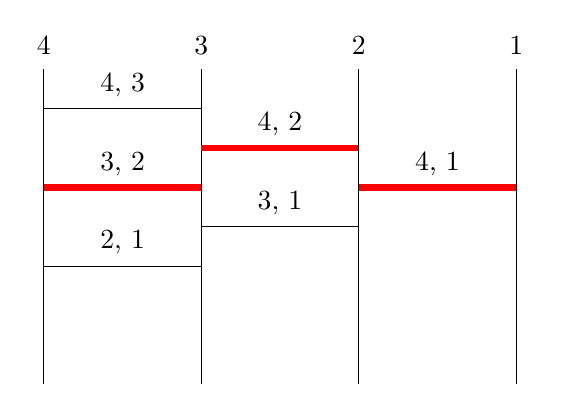
\begin{tikzpicture}
        \draw(0, 0) to (0, 4);
            \node at(0, 4.3){4};
             \draw(0, 3.5) to (2, 3.5);
                \node at(1, 3.8){4, 3};
            
            \draw[line width=0.8mm, red](0, 2.5) to (2, 2.5);
                \node at(1, 2.8){3, 2};

            \draw(0, 1.5) to (2, 1.5);
                \node at(1, 1.8){2, 1};
        \draw(2, 0) to (2, 4);
            \node at(2, 4.3){3};
                \draw[line width=.8mm, red](2, 3) to (4, 3);
                    \node at(3, 3.3){4, 2};
           
                \draw(2, 2) to (4, 2);
                    \node at(3, 2.3){3, 1};
        \draw(4, 0) to (4, 4);
             \node at(4, 4.3){2};
                \draw[line width=0.8mm, red](4, 2.5) to (6, 2.5);
                    \node at (5, 2.8){4, 1};
        \draw(6, 0) to (6, 4);
            \node at(6, 4.3){1};


    \end{tikzpicture}
    \end{center}
    \caption{The root ladder of $(4,3,2,1)$. Note that bar 4,2 is the parent of bar 3,2 and 4,1. Also note that 
    bar 3, 2 is the the left child of 4, 2 and 4, 1 is the right child.}
\end{figure}



\section{Procedure}

Thus far, the problem has been introduced and the required terminologt has been defined. Recall that there are two 
changes; the insertion/deletion of bars or repositioning bars.
However, there has yet to be discussion regarding the two 
listing algorithms. In the procedure section 
we look at each of the algorithms and explain what 
each of the algorithms are doing. The goal is to transition from 
$L_{i}$ to $L_{i+1}$ in $CanL{\pi_{N}}$ with minimal change, which means adding or removing 
the least number of bars to get from $L_{i}$ to $L_{i+1}$ or relocating 
the least number of bars to get from $L_{i}$ to $L_{i+1}$.\par 

The reason that the modified SJT and CI algorithms were chosen is because they allow 
for minimal change from $L_{i}$ to $L_{i+1}$. While conducting this research, modifications 
to the permutation listing algorithms mentioned in chapter one were applied. Recall that 
these listing algorithms were Zaks, Heaps, and Lexicographic. These listing algorithms 
did not allow for minimal change when transitioning from $L_{i}$ to $L_{i+1}$.
%%section SJT
\subsection{Steinhaus-Johnson-Trotter}
\begin{algorithm}
  \caption{Modified SJT algorithm for processing at $K=N$}
  \begin{algorithmic}[1]
    \Function{modifiedSjt}{$N$, $Ladder[2(N-1)-1][N-1]$, $Arr[N-1]$, $Direction[N]$}


      \State $print(Ladder)$

      %%base case
      \If{$globalCount = N!$}
        \State return
      \EndIf

     
      \State $dir \gets direction[N]$
      \State $K \gets N-1$
      %%swap the nth element n-1 times
      \For{$i \gets 1$,$i < N$, $i \gets i+1$}
        
        \If{$dir = left$}
            \State $row \gets (N) - i$
            \State $col \gets row$
            \State $ladder[row][col] \gets 1$
        \Else
            \State $row \gets i$
            \State $col \gets row$
            \State $ladder[row][col] \gets 0$
        \EndIf
        \State $globalCount \gets globalCount+1$
        \State $print(Ladder)$

      \EndFor
      \State $direction[N] \gets !direction[N]$
      \State $HELPERSJT(K, N, ladder, arr, direction)$
      \State $MODIFIEDSJT(N,  ladder, arr, direction)$

    \EndFunction
  \end{algorithmic}
\end{algorithm}

%%helper algorithm
\begin{algorithm}
  \caption{Helper SJT algorithm for processing when $2 \leq K < N$}
  \begin{algorithmic}[1]
    \Function{helpersjt}{$N$, $K=(N-1)$, $Ladder[2(N-1)-1][N-1]$, $Arr[N-1]$, $Direction[N]$}

      \For{$i \gets K$, $i \geq 1$, $i \gets i-1$}
        \If{$arr[K] < K$}
        \State $globalCount \gets globalCount + 1$

          \If{$dir[K] = LEFT$}
            \State $row \gets (N-1) + (N-K) - arr[K]$
            \State $col \gets (K) - arr[K]$
            \State $ladder[row][col] \gets 1$

          \Else
            \State $row \gets  (N-1) + (N-K) + arr[K] - (K-2)$
            \State $col \gets arr[K]$
            \State $ladder[row][col] \gets 0$
          \EndIf
          \State $arr[K]\gets arr[K]+1$
          \State return
        \Else 
          \State $arr[K] \gets 0$
          \State $direction[K] \gets !direction[K]$
        \EndIf
        $K \gets K-1$
      \EndFor
      \EndFunction
  \end{algorithmic}
\end{algorithm}
\pagebreak

Let the \emph{identity ladder} be the ladder for the sorted permutation from $[1 \dots N]$.
Let the initial conditions of the algorithm be the fallowing. The $Ladder= 2D array$,  
let $n \geq 1$, let $arr$ be set to zero for all indexes. Let $dir$ be set to false 
for all indexes. The principles of the algorithm are the following, if the direction for a 
given route is false, then bars will be added for that given route, from right to left, bottom to top, until no more bars can be added. Let a 
$1$ at $Ladder[row][col]$ indicate a bar has been added to the ladder at the given row and column.
If the direction for a given route is true, then bars will be removed for that given route, left to right, top to bottom, until 
no more bars can be removed. Let a $0$ at $Ladder[row][col]$ indicate a bar has been removed from the ladder 
at the given row and column. Let $K$ be the value of some given route where $1 < K <= N$. Note that element one has no route.
The number of bars for a given route is $1 \leq K < N$. This is because the maximum number of inversions 
the $kth$ element can make is $K-1$, therefore the $kth$ route can have at most $N-1$, if $K=N$, and 
at least $1$ bar if $K=2$. Once all the bars for the $Kth$ route have been added 
or removed, the direction for the $Kth$ route is switched, indicating that its bars will be removed if they 
were added, or added if they were removed. Once all the bars for the $Kth$ route have been added or removed, 
the next bar of the $K-1th$ route will be added or removed. Once this is done, the bars of route $K$ will 
then be added if they were previously removed or removed if previously added. Repeat this process until all
$N!$ ladders have been generated.


%%prove the dimensions of the datastructure
\begin{theorem}
  The number of rows required for the ladder data-structure is $2(N-1) - 1$ and the number of columns required for 
  the ladder is $N-1$.
\end{theorem}
\begin{proof}
  The number of columns is fairly straighforward. Seeing as there are always $N$ elements in $\pi_{N}$, 
  a column represents a gap between lines in the corresponding ladder-lottery. Let $Line_{i}$ be a vertical line in a ladder-lottery 
  with some element in $\pi_{N}$ at the top of the line and the $ith$ element in $\pi_{N}$ be 
  at the bottom of $Line_{i}$. There are $N$ lines in the ladder-lottery, a column in the ladder data-structure
  simply represents a gap between two adjacent lines in the ladder lottery.\par 
  The number of rows for the ladder data-structure is calculated a follows, given $\pi_{N}$, the minimal 
  number of rows required is when $\pi_{N}$ is sorted. In this case there are zero rows because there are 
  zero bars added to the ladder. This ladder is $L_{N_{ID}}$ and is 
  the first ladder in $CanL{\pi_{N}}$. When a bar is added to the ladder it can be added to an already existing row 
  or to a new row. If the current state of the ladder is $L_{N_{ID}}$ then the new bar will create the $N-1$th row in the 
  $N-1$th column. Let the bar belong to the $Nth$ route, then repeat adding bars for the $Nth$ route, bottom to top left to right. 
  Since no two bars of the $Nth$ route can be on the same row, this will require $N-1$ rows. Note, if they were added to the same 
  row, then the left end point of the right bar would be touching the right end point of the left bar which is disallowed. Once the 
  bars of the $Nth$ element are added, the bars of the $N-1th$ route will be added. The $N-1th's$ first bar 
  will be added to the $N-2$ column, otherwise it would be directly below the first bar of the $Nth$ route, which is a violation. 
  Since the first bar of the $N-1$'s element is added to column $N-2$, then it must be given a new row, otherwise its right end point 
  will be touching  the left end point of the first bar of route $N$. The remaining $N-2$ bars of element $N-1$
  will be added bottom right to top left, but none of their end points will touch the end points of element $N$ seeing as they will 
  always be two columns apart from any bar in $N's$ route. The same logic applies to element $N-2$, it will require one extra row for its 
  first bar, in order not to touch the first bar of element $N-1$, but the remainder of its bars will always be two columns away from 
  the remainder of the bars for $N-1$, etc. Therefore there are $N-2$ rows required for each element, $K$,  $2 \leq K < N$. Note that element 
  $1$ has no bars in its route. Therefore there are $(N-1)$ rows required for element $N's$ route plus $(N-2)$ rows required for 
  elements $2 \leq K < N$. In conclusion the number of rows required is $(N-1) + (N-2) = 2(N-1)-1$. See figure for the tree of ladders 
  generated by modified SJT for $N=4$
\end{proof}



\begin{figure}[!htp]
\begin{center}
  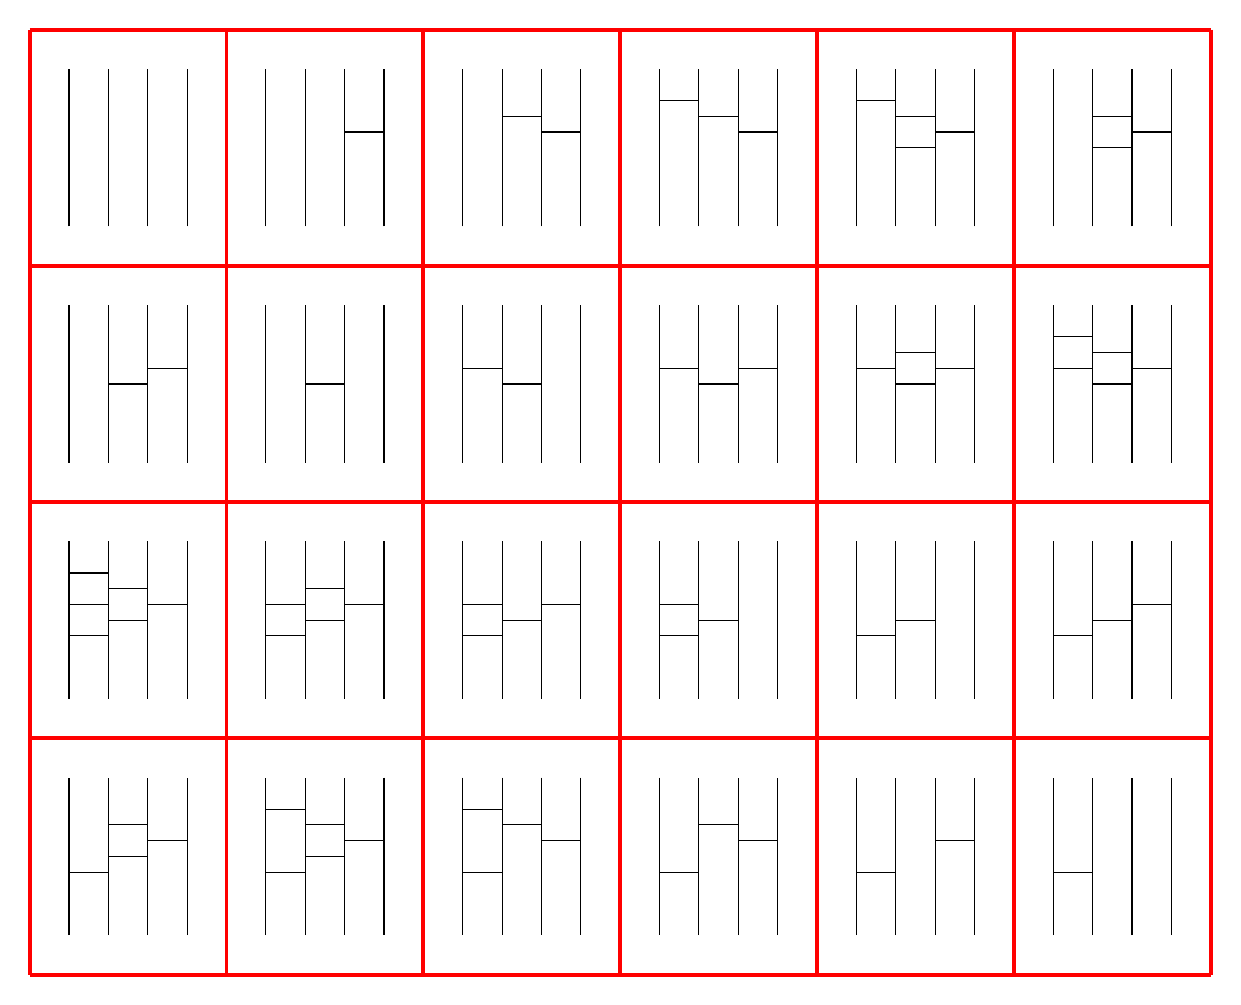
\begin{tikzpicture}
    \draw(0, 0) to (0, 2);
    \draw(0.5, 0) to (0.5, 2);
    \draw(1, 0) to (1, 2);
    \draw(1.5, 0) to (1.5, 2);

    \draw(2.5, 0) to (2.5, 2);
    \draw(3, 0) to (3, 2);
    \draw(3.5, 0) to (3.5, 2);
      \draw(3.5, 1.2) to (4, 1.2);
    \draw(4, 0) to (4, 2);

    \draw(5, 0) to (5, 2);
    \draw(5.5, 0) to (5.5, 2);
      \draw(5.5, 1.4) to (6, 1.4);
    \draw(6, 0) to (6, 2);
      \draw(6, 1.2) to (6.5, 1.2);
    \draw(6.5, 0) to (6.5, 2);

    \draw(7.5, 0) to (7.5, 2);
      \draw(7.5, 1.6) to (8, 1.6);
    \draw(8, 0) to (8, 2);
      \draw(8, 1.4) to (8.5, 1.4);
    \draw(8.5, 0) to (8.5, 2);
      \draw(8.5, 1.2) to (9, 1.2);
    \draw(9, 0) to (9, 2);

    \draw(10, 0) to (10, 2);
      \draw(10, 1.6) to (10.5, 1.6);
    \draw(10.5, 0) to (10.5, 2);
      \draw(10.5, 1.4) to (11, 1.4);
      \draw(10.5, 1) to (11, 1);
    \draw(11, 0) to (11, 2);
      \draw(11, 1.2) to (11.5, 1.2);
    \draw(11.5, 0) to (11.5, 2);

    \draw(12.5, 0) to (12.5, 2);
    \draw(13, 0) to (13, 2);
      \draw(13, 1.4) to (13.5, 1.4);
      \draw(13, 1) to (13.5, 1);
    \draw(13.5, 0) to (13.5, 2);
      \draw(13.5, 1.2) to (14, 1.2);
    \draw(14, 0) to (14, 2);

    %%End of first row
    %%Second row

    \draw(0, -3) to (0, -1);
    \draw(0.5, -3) to (0.5, -1);
      \draw(0.5, -2) to (1, -2);
    \draw(1, -3) to (1, -1);
      \draw(1, -1.8) to (1.5, -1.8);
    \draw(1.5, -3) to (1.5, -1);

    \draw(2.5, -3) to (2.5, -1);
    \draw(3, -3) to (3, -1);
      \draw(3, -2) to (3.5, -2);
    \draw(3.5, -3) to (3.5, -1);
    \draw(4, -3) to (4, -1);

    \draw(5, -3) to (5, -1);
      \draw(5, -1.8) to (5.5, -1.8);
    \draw(5.5, -3) to (5.5, -1);
      \draw(5.5, -2) to (6, -2);
    \draw(6, -3) to (6, -1);
    \draw(6.5, -3) to (6.5, -1);

    \draw(7.5, -3) to (7.5, -1);
      \draw(7.5, -1.8) to (8, -1.8);
    \draw(8, -3) to (8, -1);
      \draw(8, -2) to (8.5, -2);
    \draw(8.5, -3) to (8.5, -1);
      \draw(8.5, -1.8) to (9, -1.8);
    \draw(9, -3) to (9, -1);

    \draw(10, -3) to (10, -1);
      \draw(10, -1.8) to (10.5, -1.8);
    \draw(10.5, -3) to (10.5, -1);
      \draw(10.5, -1.6) to (11, -1.6);
      \draw(10.5, -2) to (11, -2); 
    \draw(11, -3) to (11, -1);
      \draw(11, -1.8) to (11.5, -1.8);
    \draw(11.5, -3) to (11.5, -1);

    \draw(12.5, -3) to (12.5, -1);
      \draw(12.5, -1.4) to (13, -1.4);
      \draw(12.5, -1.8) to (13, -1.8);
    \draw(13, -3) to (13, -1);
      \draw(13, -1.6) to (13.5, -1.6);
      \draw(13, -2) to (13.5, -2);
    \draw(13.5, -3) to (13.5, -1);
      \draw(13.5, -1.8) to (14, -1.8);
    \draw(14, -3) to (14, -1);
    %%End of second row
    \draw(0, -6) to (0, -4);
      \draw(0, -5.2) to (0.5, -5.2);
      \draw(0, -4.4) to (0.5, -4.4);
      \draw(0, -4.8) to (0.5, -4.8);
    \draw(0.5, -6) to (0.5, -4);
      \draw(0.5, -4.6) to (1, -4.6);
      \draw(0.5, -5) to (1, -5);
    \draw(1, -6) to (1, -4);
      \draw(1, -4.8) to (1.5, -4.8);
    \draw(1.5, -6) to (1.5, -4);

    \draw(2.5, -6) to (2.5, -4);
      \draw(2.5, -5.2) to (3, -5.2);
      \draw(2.5, -4.8) to (3, -4.8);
    \draw(3, -6) to (3, -4);
      \draw(3, -4.6) to (3.5, -4.6);
      \draw(3, -5) to (3.5, -5);
    \draw(3.5, -6) to (3.5, -4);
      \draw(3.5, -4.8) to (4, -4.8);
    \draw(4, -6) to (4, -4);

    \draw(5, -6) to (5, -4);
      \draw(5, -5.2) to (5.5, -5.2);
      \draw(5, -4.8) to (5.5, -4.8);
    \draw(5.5, -6) to (5.5, -4);
      \draw(5.5, -5) to (6, -5);
    \draw(6, -6) to (6, -4);
      \draw(6, -4.8) to (6.5, -4.8);
    \draw(6.5, -6) to (6.5, -4);

    \draw(7.5, -6) to (7.5, -4);
      \draw(7.5, -5.2) to (8, -5.2);
      \draw(7.5, -4.8) to (8, -4.8);
    \draw(8, -6) to (8, -4);
       \draw(8, -5) to (8.5, -5);
    \draw(8.5, -6) to (8.5, -4);
    \draw(9, -6) to (9, -4);

    \draw(10, -6) to (10, -4);
          \draw(10, -5.2) to (10.5, -5.2);
    \draw(10.5, -6) to (10.5, -4);
           \draw(10.5, -5) to (11, -5);
    \draw(11, -6) to (11, -4);
    \draw(11.5, -6) to (11.5, -4);

    \draw(12.5, -6) to (12.5, -4);
              \draw(12.5, -5.2) to (13, -5.2);

    \draw(13, -6) to (13, -4);
               \draw(13, -5) to (13.5, -5);

    \draw(13.5, -6) to (13.5, -4);
               \draw(13.5, -4.8) to (14, -4.8);

    \draw(14, -6) to (14, -4);

    %%End of third row

    \draw(0, -9) to (0, -7);
      \draw(0, -8.2) to (0.5, -8.2);
    \draw(0.5, -9) to (0.5, -7);
      \draw(0.5, -8) to (1, -8);
      \draw(0.5, -7.6) to (1, -7.6);
    \draw(1, -9) to (1, -7);
      \draw(1, -7.8) to (1.5, -7.8);
    \draw(1.5, -9) to (1.5, -7);

    \draw(2.5, -9) to (2.5, -7);
      \draw(2.5, -7.4) to (3, -7.4);
      \draw(2.5, -8.2) to (3, -8.2);
    \draw(3, -9) to (3, -7);
      \draw(3, -8) to (3.5, -8);
      \draw(3, -7.6) to (3.5, -7.6);
    \draw(3.5, -9) to (3.5, -7);
       \draw(3.5, -7.8) to (4, -7.8);
    \draw(4, -7) to (4, -9);

    \draw(5, -7) to (5, -9);
      \draw(5, -7.4) to (5.5, -7.4);
      \draw(5, -8.2) to (5.5, -8.2);
    \draw(5.5, -7) to (5.5, -9);
      \draw(5.5, -7.6) to (6, -7.6);
    \draw(6, -7) to (6, -9);
           \draw(6, -7.8) to (6.5, -7.8);
    \draw(6.5, -7) to (6.5, -9);

    \draw(7.5, -7) to (7.5, -9);
          \draw(7.5, -8.2) to (8, -8.2);
    \draw(8, -9) to (8, -7);
        \draw(8, -7.6) to (8.5, -7.6);
    \draw(8.5, -9) to (8.5, -7);
               \draw(8.5, -7.8) to (9, -7.8);
    \draw(9, -9) to (9, -7);

    \draw(10, -9) to (10, -7);
      \draw(10, -8.2) to (10.5, -8.2);
    \draw(10.5, -9) to (10.5, -7);
    \draw(11, -9) to (11, -7);
      \draw(11, -7.8) to (11.5, -7.8);
    \draw(11.5, -9) to (11.5, -7);

    \draw(12.5, -9) to (12.5, -7);
              \draw(12.5, -8.2) to (13, -8.2);
    \draw(13, -9) to (13, -7);
    \draw(13.5, -9) to (13.5, -7);
    \draw(14, -9) to (14, -7);

    %%end fourth row

    %%draw the border

    \draw [line width=0.5mm, red ] (-0.5,2.5) to (-0.5,-9.5);
    \draw [line width=0.5mm, red ] (2,2.5) to (2,-9.5);
    \draw [line width=0.5mm, red ] (4.5,2.5) to (4.5,-9.5);
    \draw [line width=0.5mm, red ] (7,2.5) to (7,-9.5);
    \draw [line width=0.5mm, red ] (9.5,2.5) to (9.5,-9.5);
    \draw [line width=0.5mm, red ] (12,2.5) to (12,-9.5);
    \draw [line width=0.5mm, red ] (14.5,2.5) to (14.5,-9.5);

   \draw [line width=0.5mm, red ] (-0.5,2.5) to (14.5,2.5);
   \draw [line width=0.5mm, red ] (-0.5,-0.5) to (14.5,-0.5);
      \draw [line width=0.5mm, red ] (-0.5,-3.5) to (14.5,-3.5);
   \draw [line width=0.5mm, red ] (-0.5,-6.5) to (14.5,-6.5);
   \draw [line width=0.5mm, red ] (-0.5,-9.5) to (14.5,-9.5);





  \end{tikzpicture}
  \end{center}
  \caption{The table of $CanL{\pi_{4}}$ generated using the modified SJT algorithm. The table is to be read from top left to bottom right. Note that each ladder is the root ladder from each corresponding $OptL{\pi_{4}}$}
\end{figure}

%%end proof


From the above figure, it should be clear that the canonical representative from $CanL{\pi_{N}}$ when using the 
modified SJT algorithm is the root ladder from each $OptL{\pi_{N}}$. Recall that the root ladder is the 
ladder whose bars of a lesser route have not crossed the bars of a greater route. In the case of the 
modified sjt algorithm, transitioning from $L_{i}$ to $L_{i+1}$ involves simply inserting a new bar 
or removing a bar for a given route. Let $K$ be the current route. If a new bar being added belongs to 
route $K$, then the addition of the bar does not violate the property of the root ladder. If the new bar to
be added belongs to route $K-1$, then the bar is added below $K's$ bars, still not violating the property of 
the root ladder. When a bar is removed, that implies it has already been added. Let $L_{i}$ be a 
ladder whose bar is about to be removed, thus transitioning to $L_{i+1}$. Let $L_{i}$ be a root ladder
, then removing a bar from $L_{i}$ cannot make $L_{i+1}$ a non-root ladder, because 
removing a bar from $L_{i}$ does not allow the bar of a lesser element to cross the bars of a greater element.
Thus, the canonical representative for $CanL{\pi_{N}}$ is always the root ladder from each $OptL{\pi_{N}}$.\par 



%%Beging the cases
The calculations for the row and column for the bar 
depend on several factors. The first factor is whether the row and column is being calculated for $K=N$ or 
if $K < N$. If $K=N$, then the row and column are calculated using the main function, modifiedSJT. The second factor 
is whether a bar is being removed from the ladder or a bar is being added to the ladder. Therefore, there are eight cases 
to consider. The cases are the following: 
\begin{caseof}
  \case{$Route = N$}{Bar is being added. Row is being calculated.}
  \case{$Route = N$}{Bar is being added. Column is being calculated.}
  \case{$Route = N$}{Bar is being removed. Row is being calculated.}
  \case{$Route = N$}{Bar is being removed. Column is being calculated.}
  \case{$Route < N$}{Bar is being added. Row is being calculated.}
  \case{$Route < N$}{Bar is being added. Column is being calculated.}
  \case{$Route < N$}{Bar is being removed. Row is being calculated.}
  \case{$Route < N$}{Bar is being removed. Column is being calculated.}
\end{caseof}

%%End the cases

When proving the above cases, keep in mind that the ladder, $L$, is a two dimensional array with $2(N-1)-1$ rows and $(N-1)$ columns.

%%proof 1
\begin{lemma}
  Let $route=N$. Let $I=$ the current number of bars in the ladder belonging to route $N$. 
  Assume a bar is being added. Then the $row=(N-1)-I$.
\end{lemma}
\begin{proof}
  Keeping in mind we are only dealing with root ladders, then the bars of the $Nth$ route will be above the bars of 
  any other route. The bars are added bottom right to top left, and no two bars of the $Nth$ route can be on the same row, 
  for having two bars of the same route on the same row violates the constraint that no two endpoints of two bars can be toucing.
  There are a total of $N-1$ rows requried for the bars of the $Nth$ route. $I$ is incremented for each bar that is added 
  to the $Nth$ route. The first bar to be added will be at row $N-1$, once it is added $I$ is incremented by one, the second 
  bar of the $Nth$ route will be added to row $N-2$, which equals $N-1-I$. Then $I$ is incremented again. This continues 
  until all bars of the $Nth$ route are added. Refer to figure --fig for an example of row calulation when adding a bar 
  for the $Nth$ route.
\end{proof}\pagebreak


\begin{figure}[!htp]
  \begin{center}
    \begin{tikzpicture}
      \draw(0, 0) to (0, 6);
      \draw(2, 0) to (2, 6);
        \node at(3, 4.7){4,2};
        \draw(2, 4.5) to (4, 4.5);
      \draw(4, 0) to (4, 6);
        \node at(5, 3.7){4,3};
        \draw(4, 3.5) to (6, 3.5);
      \draw(6, 0) to (6, 6);

      \node at(-2, 5.5){R1};
      \node at(-2, 4.5){R2};
      \node at(-2, 3.5){R3};
      \node at(-2, 2.5){R4};
      \node at(-2, 1.5){R5};

      \node at(0, 6.2){1};
      \node at(2, 6.2){4};
      \node at(4, 6.2){2};
      \node at(6, 6.2){3};

      \draw (1,5.5) ellipse (1cm and .4cm);

    \end{tikzpicture}
  \end{center}
  \caption{The row of the last bar to be added for element $4$ is row $1$. $row=1=3-2=(N-1)-I$}
\end{figure}

%%end proof 1


%%Prove case 2
\begin{lemma}
  Let $route=N$. Let $I=$ the current number of bars in the ladder belonging to route $N$. 
  Assume a bar is being added. Then the $column=(N-1)-I$.
\end{lemma}
\begin{proof}
  Keeping in mind we are only dealing with root ladders, then the bars of the $Nth$ route will be above the bars of 
  any other route. The bars are added bottom right to top left. The ladder has a total of $N-1$ columns, seeing as 
  the $Nth$ element has $N-1$ bars, each requiring their own column. If two bars of the $Nth$ element were 
  in the same column, then this would violate one of two constraints. Either the two bars would be directly 
  above/below each other, in which case the ladder would not be optimal seeing as the two elements that crossed the 
  top bar would then cross the bottom bar, which means the ladder has an extra bar. The second case can be discredited as 
  follows. Let the top bar belonging to route $N$ be designated as $X$, let the bottom bar belonging to route $N$ be 
  designated as $Y$. Assume $X$ and $Y$ are in the same column.
  Then there is some third bar $Z$, not belonging to route $N$ and not in the same column 
  as $X$ and $Y$ such that $Z$ is in the column directly to the left or right of the column of $X$ and $Y$. But if that 
  is the case, then $Z$ is above bar $Y$ which violates the definition of the root ladder. Therefore, every bar 
  belonging to route $N$ requires its own column. The first bar to be added to route $N$ goes in the rightmost column which 
  equals column $N-1$, then $I$ is incremented by one. The second bar is in columb $(N-1)-1=(N-1)-I$ and $I$ is incremented 
  by one. The process continues until all $(N-1)$ bars of the $Nth$ route have been added. See figure --fig for an example 
  of column calculation.
\end{proof}

\begin{figure}[!htp]
  \begin{center}
    \begin{tikzpicture}
       \draw(0, 0) to (0, 6);
      \draw(2, 0) to (2, 6);
        \node at(3, 4.7){4,2};
        \draw(2, 4.5) to (4, 4.5);
      \draw(4, 0) to (4, 6);
        \node at(5, 3.7){4,3};
        \draw(4, 3.5) to (6, 3.5);
      \draw(6, 0) to (6, 6);

      \node at(1, -0.3){Col 1};
      \node at(3, -0.3){Col 2};
      \node at(5, -0.3){Col 3};

      \node at(0, 6.2){1};
      \node at(2, 6.2){4};
      \node at(4, 6.2){2};
      \node at(6, 6.2){3};

      \draw (1,5.5) ellipse (1cm and .4cm);


      
    \end{tikzpicture}
  \end{center}
  \caption{The column of the last bar to be added for element $4$ is $1$. $column=1=3-2=(N-1)-I$}
\end{figure}
%%End proof of case 2


%%Proof of case 3
\begin{lemma}
  Let $route=N$. Let $I=$ the current number of bars that have been removed from route $N$. Assume a bar is being removed. 
  Then the $row=I+1$
\end{lemma}
\begin{proof}
  Keeping in mind we are dealing with root ladders and bars are removed from left to right, top to bottom, then the first bar to 
  be removed from route $N$ is at row one. Since no bars have been removed, $I$ currently equals zero, 
  thus row $1=I+1$. Once removed, $I$ is increased by one, indicating a bar has been removed. The next bar is at row two, 
  which again equals $I+1$. Continue until all bars of the $Nth$ route have been removed. See figure --fig for an example 
  of row calculation when removing a bar for the $Nth$ element.
\end{proof}
\begin{figure}[!htp]
  \begin{center}
    \begin{tikzpicture}
      \draw(0, 0) to (0, 6);
        \draw [dashed] (0,5.5) -- (2,5.5);
      \draw(2, 0) to (2, 6);
        \node at(3, 4.7){4,2};
        \draw(2, 4.5) to (4, 4.5);
      \draw(4, 0) to (4, 6);
        \node at(5, 3.7){4,3};
        \draw(4, 3.5) to (6, 3.5);
      \draw(6, 0) to (6, 6);

      \node at(-2, 5.5){R1};
      \node at(-2, 4.5){R2};
      \node at(-2, 3.5){R3};
      \node at(-2, 2.5){R4};
      \node at(-2, 1.5){R5};

      \node at(0, 6.2){1};
      \node at(2, 6.2){4};
      \node at(4, 6.2){2};
      \node at(6, 6.2){3};

      \draw (3,4.5) ellipse (1cm and .4cm);

    \end{tikzpicture}
  \end{center}
  \caption{The row of the second bar to be removed from element $4's$ route is row $2$. The dashed bar indicates that it has already been 
  removed from $4's$ route. $I$ is the number of bars currently removed from $4's$ route, which is currently $1$. Therefore $row=2=I+1$}
\end{figure}

%%End of proof of case 3


%%Proof Case 4
\begin{lemma}
  Let $route=N$. Let $I=$ the current number of bars that have been removed from route $N$. Assume a bar is being removed.
  Then the $column=I+1$.
\end{lemma}
\begin{proof}
  Keeping in mind we are dealing with root ladders and bars are removed from left to right, top to bottom, then the first bar to 
  be removed from route $N$ is at column one. Since no bars have been removed, $I$ currently equals zero, 
  thus column $1=I+1$. Once removed, $I$ is increased by one, indicating a bar has been removed. The next bar is at column two, 
  which again equals $I+1$. Continue until all bars of the $Nth$ route have been removed. See figure --fig for an example 
  of column calculation when removing a bar from the $Nth$ route.
\end{proof}

\begin{figure}[!htp]
  \begin{center}
    \begin{tikzpicture}
      \draw(0, 0) to (0, 6);
        \draw [dashed] (0,5.5) -- (2,5.5);

      \draw(2, 0) to (2, 6);
        \node at(3, 4.7){4,2};
        \draw(2, 4.5) to (4, 4.5);
      \draw(4, 0) to (4, 6);
        \node at(5, 3.7){4,3};
        \draw(4, 3.5) to (6, 3.5);
      \draw(6, 0) to (6, 6);

      \node at(1, -0.3){Col 1};
      \node at(3, -0.3){Col 2};
      \node at(5, -0.3){Col 3};

      \node at(0, 6.2){1};
      \node at(2, 6.2){4};
      \node at(4, 6.2){2};
      \node at(6, 6.2){3};

      \draw (3,4.5) ellipse (1cm and .4cm);


      
    \end{tikzpicture}
  \end{center}
  \caption{The column of the second bar to be removed from element $4's$ route is row $2$. The dashed bar indicates that it has already been 
  removed from $4's$ route. $I$ is the number of bars currently removed from $4's$ route, which currently is $1$. Therefore $column=2=I+1$}
\end{figure}
%%End of proof of case 4



%%Proof of case 5
\begin{lemma}
  Let $arr$ be a one indexed array. Let $2 \leq K < N$ be the $Kth$ element to have a bar added to its route. 
  Let $arr[K]$ represent the number of bars for route $K$ that are currently in the 
  ladder. Let $L_{i}$ be a two dimensional, one indexed array representing the current ladder.
  The the row for the current bar to be added for route $K$ is $Row=(N-1) + (N-K) - arr[K]$.
\end{lemma}
\begin{proof}
   It must be noted that we are listing only root ladders. So when transitioning from 
$L_{i}$ to $L_{i+1}$ in $CanL{\pi_{N}}$ both are root ladders. Recall that the root ladder is the ladder such that no  
route of any lesser value in $\pi$ has crossed the route of a greater value. With this in mind, one can say that the 
number of rows required for the $Nth$ value is $N-1$ seeing as the $Nth$ value can have at most $N-1$ bars in its route, each requiring  their own 
row. Since bars are added right to left, bottom, up, then the first bar of route $K$ will be added to the row 
just  below the last bar of the previous route. The reason $N-1$ is added is because the $Nth$ element requires 
$N-1$ rows in $L$. If $K$ is one less than $N$ then 
the first bar of $K$ will be added one row below the last bar of $N$. If $K$ is two less than $N$ then the first bar 
of $K$ will be added two rows below the last bar of $N$, etc. The $(N-K)$ is added because 
the difference between $N$ and $K$ is the offset of the difference in rows between the lowest/first bar of $N$ 
and the lowest/first bar of $K$. When a bar is added to $K's$ route, the $arr[k]$ is incremented by one. This value is subtracted in 
order to effectively move up the ladder as bars are added to $K's$ route from bottom right to top left. See figure for an example of 
row calculation when adding a bar for $K < N$.
\end{proof}\pagebreak

\begin{figure}[!htp]
  \begin{center}
    
    \begin{tikzpicture}

    \draw(0, -2) to (0, 6);
       \draw(0, 5.5) to (2, 5.5);
       \node at (1, 5.7){5,1};
       \node at (-1, 5.5){R1};
     \draw(2, -2) to (2, 6);
       \draw(2, 4.5) to (4, 4.5);
       \draw(2, 0.5) to (4, 0.5);
       \node at (3, 4.7){5,3};
       \node at(3, 0.7){3, 2};
       \node at(-1, 4.5){R2};
     \draw(4, -2) to (4, 6);
       \draw(4, 3.5) to (6, 3.5);
       \node at(5, 3.7){5,2};
       \node at(-1, 3.5){R3};
     \draw(6, -2) to (6, 6);
       \draw(6, 2.5) to (8, 2.5);
       \node at(7, 2.7){5,4};
       \node at(-1, 2.5){R4};
     \draw(8, -2) to (8, 6);

    \node at(-1, 1.5){R5};
    \node at(-1, 0.5){R6};
    \node at(-1, -0.5){R7};
    \draw (1,1.5) ellipse (1cm and .4cm);

  \end{tikzpicture}

\end{center}
\caption{The second bar of route 3 goes will go in row 5, column 1. $5 = (5-1)+(5-3)-1 = (N-1)+(N-K)-arr[K]$.}
\end{figure}
%%End of prof of case 5


%%Proof of case 6
\begin{lemma}
  Let $arr$ be a one indexed array. Let $2 \leq K < N$ be the $Kth$ element to have a bar added to its route. 
  Let $arr[K]$ represent the number of bars for route $K$ that are currently in $L$. 
  The the column for the current bar to be added for route $K$ is $Column=(K-1)-arr[K]$.
\end{lemma}
\begin{proof}
  The total number of bars required for route $K$ is $K-1$, each requring their own column. The reason each 
  bar requires its own column is the same for when the route equals $N$. See the proof for lemma 3.1.5. The 
  bars are added right to left and when a bar is added $arr[K]$ is incremented by one. The initial column to add the first bar 
  of route $K$ is column $K-1$. This is because the first bar of the $Kth$ route is the left child bar of the 
  lowest bar of the $K+1th$ route. Denote the first bar to be added of the $Kth$ route as $Y$ and the 
  lowest bar of the $K+1th$ route as $X$. $X$ is the parent bar of $Y$ and $Y$ is the left child bar of 
  $X$ for the following reasosn. If $Y$ was directly below $X$, then the ladder would have redundant bars, thus making it 
  non-optimal. If $Y$ was to the right of $X$, then $Y$ would either be above $X$, thus violating the property of the root ladder, 
  or if $Y$ were below $X$ and to the right of $X$ then $Y$ would be part of the route for $K+1$, yet this is a contradiction 
  seeing as we said $Y$ belongs to $K's$ route. Therefore, $Y$ must be in a column to the left of $X$. As bars are added 
  to $K's$ route, $arr[K]$ is incremented for each bar. It is subtracted from the original column, $K-1$, effectively moving 
  to the next column to the left in $L$. See figure --fig for an example of column calculation when adding a bar for $K<N$.
\end{proof}
\begin{figure}[!htp]
  \begin{center}
    
    \begin{tikzpicture}

    \draw(0, -2) to (0, 6);
       \draw(0, 5.5) to (2, 5.5);
       \node at (1, 5.7){5,1};
     \draw(2, -2) to (2, 6);
       \draw(2, 4.5) to (4, 4.5);
       \draw(2, 0.5) to (4, 0.5);
       \node at (3, 4.7){5,3};
       \node at(3, 0.7){3, 2};
     \draw(4, -2) to (4, 6);
       \draw(4, 3.5) to (6, 3.5);
       \node at(5, 3.7){5,2};
     \draw(6, -2) to (6, 6);
       \draw(6, 2.5) to (8, 2.5);
       \node at(7, 2.7){5,4};
     \draw(8, -2) to (8, 6);

    \draw (1,1.5) ellipse (1cm and .4cm);

    \node at(1, -2.3){Col 1};
    \node at(3, -2.3){Col 2};
    \node at(5, -2.3){Col 3};
    \node at(7, -2.3){Col 4};
  \end{tikzpicture}
\end{center} 
\caption{The second bar of route $K=3$ goes will go in column 1. Since one bar has been added, $arr[3]=1$. $col=1=2-1=(K-1)-arr[K]$.}
\end{figure}

%%End of proof of case 6


%%Proof of case 7
\begin{lemma}
  Let $arr$ be a one indexed array. Let $2 \leq K < N$ be the $Kth$ element to have a bar removed from its route. 
  Let $arr[K]$ represent the number of bars for route $K$ that have currently been removed from the ladder. 
  The the row for the current bar to be removed for route $K$ is $Row=(N-1) + (N-K) + arr[K] - (K-2)$.
\end{lemma}
\begin{proof}
  When removing a bar the row is calculated as follows. Keeping in mind bars are removed from top to bottom, left to right.
  The $Nth$ element requries the first $(N-1)$ rows. Which is why $(N-1)$ is added. The last bar to be removed of the $Kth$ route is $(N-K)$
  rows below row $(N-1)$ which is why $(N-K)$ is added. $arr[K]$ is added to effectively move down the ladder 
  for each remaining bar of the $Kth$ route in the ladder left to be removed. Since the first bar of the $Kth$ route 
  to be removed is highest up the ladder, every subsequent bar to be removed from the $Kth$ route requires 
  moving down the ladder from the row of first bar of the $Kth$ route; this is accomplished by adding $array[K]$ which 
  indicates how many bars are currently removed from the $Kth$ route. Lastly, $(K-2)$  is subtracted in order to 
  get to the row of the first bar of the $Kth$ route. The difference between the row of the last bar of the $Kth$ route and 
  the first bar of the $Kth$ route is $K-2$. Seeing as the $Kth$ route has at most $K-1$ bars, each requiring their own row, then the 
  first bar of the $Kth$ route is $K-2$ rows higher than the last bar of the $Kth$ route. See figure fig for 
  an example of removing a bar.\pagebreak
\end{proof}

\begin{figure}[!htp]
  \begin{center}
    \begin{tikzpicture}
      \draw(0, 0) to (0, 8);
        \draw(0, 7) to (2, 7);
          \node at (1, 7.3){5,4};
          \draw [dashed] (0,5) -- (2,5);

        \draw(0, 1) to (2, 1);
          \node at (1, 1.3){2, 1};
        
      
      \draw(2, 0) to (2, 8);
        \draw(2, 6) to (4, 6);
          \node at (3, 6.3){5, 2};
        \draw(2, 4) to (4, 4);
          \node at (3, 4.3){4, 1};
      \draw(4, 0) to (4, 8);
        \node at(5, 5.3){5, 1};
        \draw(4, 5) to (6, 5);
          \node at(5, 3.3){4, 3};
        \draw(4, 3) to (6, 3);
      
      \draw(6, 0) to (6, 8);
        \draw(6, 4) to (8, 4);
        \node at (7, 4.3){5, 3};
      \draw(8, 0) to (8, 8);

      \node at (-2, 7){R1};

      \node at (-2, 6){R2};

      \node at (-2, 5){R3};
      \node at(-2, 4){R4};
      \node at (-2, 3){R5};
      \node at (-2, 2){R6};
      \node at(-2, 1){R7};
      \draw (3,4) ellipse (1cm and .4cm);

    \end{tikzpicture}
  \end{center}
  \caption{The bar to be removed for route $K=4$ is (4, 1) which is at row 4. The dashed line indicates a bar 
  from route $4$ has already been removed. $row= 4 = (5-1)+(5-4)+ 1 - (2) = (N-1)+(N-K) + arr[K] - (K-2)$.}
\end{figure}
%%End of proof of case 7

%%Proof of case 8
\begin{lemma}
   Let $arr$ be a one indexed array. Let $2 \leq K < N$ be the $Kth$ element to have a bar removed from its route. 
  Let $arr[K]$ represent the number of bars for route $K$ that have currently been removed from the ladder. 
  Then the column for the current bar to be removed for route $K$ is $Column=arr[K]+1$.
\end{lemma}
\begin{proof}
  The bars are removed left to right. The first bar to be removed is the leftmost bar belonging to route $K$ which 
  is always at column $1$. This is because the number of columns required for the $K-1$ bars is $K-1$, terminating at 
  column number $K-1$. Thus, the first bar to be removed must always be at column $1$ and the last bar to 
  be removed is at column $K-1$. $arr[K]$ is incremented for each bar removed from the route of $K$.
\end{proof}

\begin{figure}[!htp]
  \begin{center}
    \begin{tikzpicture}
      \draw(0, 0) to (0, 8);
        \draw(0, 7) to (2, 7);
          \node at (1, 7.3){5,4};
          \draw [dashed] (0,5) -- (2,5);

        \draw(0, 1) to (2, 1);
          \node at (1, 1.3){2, 1};
        
      
      \draw(2, 0) to (2, 8);
        \draw(2, 6) to (4, 6);
          \node at (3, 6.3){5, 2};
        \draw(2, 4) to (4, 4);
          \node at (3, 4.3){4, 1};
      \draw(4, 0) to (4, 8);
        \node at(5, 5.3){5, 1};
        \draw(4, 5) to (6, 5);
          \node at(5, 3.3){4, 3};
        \draw(4, 3) to (6, 3);
      
      \draw(6, 0) to (6, 8);
        \draw(6, 4) to (8, 4);
        \node at (7, 4.3){5, 3};
      \draw(8, 0) to (8, 8);


      \node at (1, -0.3){Col 1};
      \node at(3, -0.3){Col 2};
      \node at (5, -0.3){Col 3};
      \node at (7, -0.3){Col 4};
      \draw (3,4) ellipse (1cm and .4cm);

    \end{tikzpicture}
  \end{center}
  \caption{The bar to be removed for route $K=4$ is (4, 1) which is at column 2. The dashed line indicates a bar 
  from route $4$ has already been removed. Since one bar from routr $4$ has been removed, $arr[4]=1$. $column= 2 = 1+1 = arr[K] + 1$.}
\end{figure}
%%End of proof of case 8
\subsection{Cyclic Inversion}
\begin{algorithm}
  \caption{First part of the algorithm Cyclic Inversion}
  \begin{algorithmic}[1]
    \Function{CyclicInversion}{$Ladder[2(N-1)-1][N-1]$, $CurrentLimit$, $MaxLimit$, $N$, $K$}


      
      %%base case
      \If{the number of bars in $Ladder=CurrentLimit$}
        \State $print(Ladder)$
        \State return
      \EndIf

      %%
      \If{$CurrentLimit > MaxLimit$}
        \State return
      \EndIf

      %%If K=N
     \If{$K=N$}

      \State {$M \gets 0$}
      \State $Row \gets K-1$
      \State $Col \gets K-1$
      \State $NumBars \gets$ current number of bars in $Ladder$
      %%While
      \While{$NumBars < CurrentLimit$ AND $M < K-1$}
        \State $Ladder[Row][Col] \gets 1$
        \State $Row \gets row-1$
        \State $Col \gets col-1$
        \State $M \gets M+1$
        \State $NumBars \gets NumBars+1$
      \EndWhile
      %%End while

      \If{$NumBars = CurrentLimir$}
        \State $PrintLadder(Ladder)$
      \EndIf
      \State remove upper leftmost bar belonging to $K's$ route.
      \State return

    \algstore{aaa}

  \end{algorithmic}
\end{algorithm}

\begin{algorithm}
  \caption{Cyclic Inversion Continued}
    \begin{algorithmic}[1]
          \algrestore{aaa}

    \Else 
      \State $count \gets 0$
      \For{$I \gets 0$, $I < K$, $I \gets I+1$}
       \If{the number of bars in $Ladder=CurrentLimit$}
            \State break
        \EndIf

        \If{$I = 0$}
          \State CyclicInversion(Ladder, CurrentLimit, MaxLimit, N, $K+1$)
      
       
        
        \Else
          \State $Row \gets (N-1) + (N-K) - count$
          \State $Column \gets (K-1)-arr[K]$
          \State $Ladder[Row][Col] \gets 1$
          \State $count \gets count + 1$
          \State CyclicInversion(Ladder, CurrentLimit, MaxLimit, N, $K+1$)
        \EndIf
      \EndFor
      \State remove all bars from $K's$ route.

    \EndIf
    \EndFunction
  \end{algorithmic}
\end{algorithm}


\begin{algorithm}
  \caption{Driver for the Cyclic Inversion Algorithm}
  \begin{algorithmic}[1]
    \Function{Cylclic Inversion Driver}{$Ladder[2(N-1)-1][N-1]$, $N$}
      \State $MaxLimit \gets (N(N-1))/2$
      \State $K \gets 2$
      \For{$I \gets 0, I <= MaxLimit, I \gets I+1$}
        \State CyclicInversion($Ladder$, $CurrentLimit \gets I$, $MaxLimit$, $N$, $K$)

      \EndFor

    \EndFunction
  \end{algorithmic}
\end{algorithm}\pagebreak

The initial conditions for the algorithm are the following. Let $Ladder$ be initialized as a two dimensional array with $2(N-1)-1$ rows and $(N-1)$ columns.  Let $N$ be initialized to the maximal element in $\pi_{N}$. Let $K$ be initialized to $2$.
Let the $MaxLimit$ be initialized to $(N(N-1))/2$.Let the $CurrentLimit$ be initialized to zero. The way the algorithm works is the following. The $CurrentLimit$ 
represents the number of bars to be inserted into $Ladder$. Once all ladders with $CurrentLimit$ bars have been created, the $CurrentLimit$ is increased by one 
and the algorithm repeats until $CurrenLimit > MaxLimit$. This creates all ladders in $CanL{\pi_{N}}$. The ladders are generated as a forest structure,
 with each value of $CurrentLimit$ creating its own tree of ladders. See figure --fig for the 
forest of ladders for $N=4$. The forest of ladders is all the ladders in $CanL{\pi_{N}}$. On each recursive call to the function, $K$ is increased by one until $K=N$. When $K=N$ all the remaining bars that need to 
be added to the ladder are added to $K=N's$ route. Then the bars of $K=N's$ route are removed and relocated to the bars of $K-1's$ route. This process 
repeats itself until all the combinations of bars for the $CurrentLimit$ are inserted. Each combination of bars into the $Ladder$ 
data structure creates a unique ladder from each $OptL{\pi_{N}}$, thus adding one more ladder to $CanL{\pi_{N}}$.
Once complete, the tree of ladders terminates, and the $CurrentLimit$ increases, thus creating a new tree in the forest for 
$CanL{\pi_{N}}$.\pagebreak

\begin{figure}[!htp]
  %%first tree
 
      
     
    \begin{minipage}{.8\textwidth}
     
         \begin{tikzpicture}
          \node at (-1, 1){\tiny $bars=0$};
          \draw(0, 0) to (0, 1);
          \draw(0.2, 0) to (.2, 1);
          \draw(.4, 0) to (.4, 1);
          \draw(.6, 0) to (.6, 1);
        \end{tikzpicture}\hspace{20mm}
     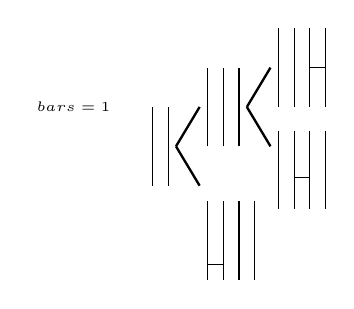
\begin{tikzpicture}
        \node at (-1, 1){\tiny $bars=1$};
        %%l1
          \draw(0, 0) to (0, 1);
          \draw(.2, 0) to (.2, 1);
                      \draw[line width=0.3mm] (.3, .5) to (.6, 1);
                      \draw[line width = .3mm](.3, .5) to (.6, 0);
          %%l2
          \draw(.7, .5) to (.7, 1.5);
          \draw(.9, .5) to (.9, 1.5);
          \draw(1.1, 0.5) to (1.1, 1.5);


            \draw[line width = .3mm](1.2, 1) to (1.5, 1.5);
            \draw[line width = .3mm](1.2, 1) to (1.5, 0.5);
          %%t3 terminate
          \draw(1.6, 1) to (1.6, 2);
          \draw(1.8, 1) to (1.8, 2);
          \draw(2, 1) to (2, 2);
            \draw(2, 1.5) to (2.2, 1.5);
          \draw(2.2, 1) to (2.2, 2);

          %l4 terminate
          \draw(.7, -0.2) to (.7, -1.2);
            \draw(.7, -1) to (.9,-1);
          \draw(.9, -.2) to (.9, -1.2);
          \draw(1.1, -.2) to (1.1, -1.2);
          \draw(1.3, -0.2) to (1.3, -1.2);

          %l5 terminate
          \draw(1.6, .7) to (1.6, -.3);
          \draw(1.8, .7) to (1.8, -.3);
            \draw(1.8, .1) to (2, .1);
          \draw(2, .7) to (2, -.3);
          \draw(2.2, .7) to (2.2, -.3);
        
      \end{tikzpicture}
      

               
    \end{minipage}\\~\\

   %%t3
  \begin{minipage}{.8\textwidth}
     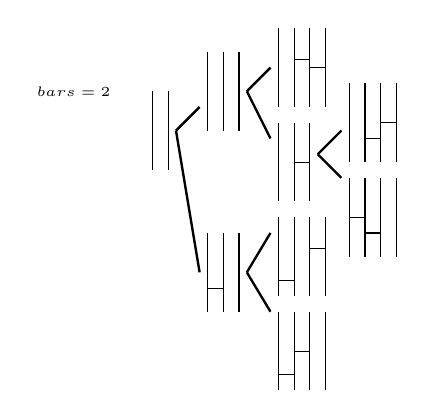
\begin{tikzpicture}
       \node at (-1, 1){\tiny $bars=2$};

        %%L1
        \draw(0, 0) to (0, 1);
        \draw(.2, 0) to (.2, 1);
        
          \draw[line width=.3mm] (.3, .5) to (.6, .8);
          \draw[line width = .3mm](.3, .5) to (.6, -1.3);

        
        \draw(.7, -.8) to (.7, -1.8);
          \draw(.7, -1.5) to (.9, -1.5);
        \draw(.9, -.8) to (.9, -1.8);
        \draw(1.1, -.8) to (1.1, -1.8);

          \draw[line width = .3mm](1.2, -1.3) to (1.5, -.8);
          \draw[line width = .3mm](1.2, -1.3) to (1.5, -1.8);
        
        %%terminate
        \draw(1.6, -.6) to (1.6, -1.6); 
          \draw(1.6, -1.4) to (1.8, -1.4);
         \draw(1.8, -.6) to (1.8, -1.6);  
         \draw(2, -.6) to (2, -1.6);  
            \draw(2, -1) to (2.2, -1); 
         \draw(2.2, -.6) to (2.2, -1.6);
         
         %%terminate
         \draw(1.6, -1.8) to (1.6, -2.8);
          \draw(1.6, -2.6) to (1.8, -2.6);
         \draw(1.8, -1.8) to (1.8, -2.8);
          \draw(1.8, -2.3) to (2, -2.3);
         \draw(2, -1.8) to (2, -2.8);
         \draw(2.2, -1.8) to (2.2, -2.8);



        %%L2 
        \draw(.7, .5) to (.7, 1.5);
        \draw(.9, .5) to (.9, 1.5);
        \draw(1.1, .5) to (1.1, 1.5);

          \draw[line width = .3mm](1.2, 1) to (1.5, 1.3);
          \draw[line width = .3mm](1.2, 1) to (1.5, .4);
        
        %%L3 terminate
        \draw(1.6, .8) to (1.6, 1.8);
        \draw(1.8, .8) to (1.8, 1.8);
          \draw(1.8, 1.4) to (2, 1.4);
        \draw(2, .8) to (2, 1.8);
          \draw(2, 1.3) to (2.2, 1.3);
        \draw(2.2, .8) to (2.2, 1.8);

        %L4 
        \draw(1.6, .6) to (1.6, -.4);
        \draw(1.8, .6) to (1.8, -.4);
          \draw(1.8, .1) to (2, .1);
        \draw(2, .6) to (2, -.4);
          \draw[line width = .3mm](2.1, .2) to (2.4, .5);
          \draw[line width = .3mm](2.1, .2) to (2.4, -.1);
        
        %L5 terminate
        \draw(2.5, .1) to (2.5, 1.1);
        \draw(2.7, .1) to (2.7, 1.1);
          \draw(2.7, .4) to (2.9, .4);
        \draw(2.9, .1) to (2.9, 1.1);
          \draw(2.9, .6) to (3.1, .6);
        \draw(3.1,.1) to (3.1, 1.1);

        %L6 terminate
        \draw(2.5, -.1) to (2.5, -1.1);
          \draw(2.5, -.6) to (2.7, -.6);
        \draw(2.7, -.1) to (2.7, -1.1);
          \draw(2.7, -.8) to (2.9, -.8);
        \draw(2.9, -.1) to (2.9, -1.1);
        \draw(3.1, -.1) to (3.1, -1.1);


      \end{tikzpicture}\hspace{10mm}
      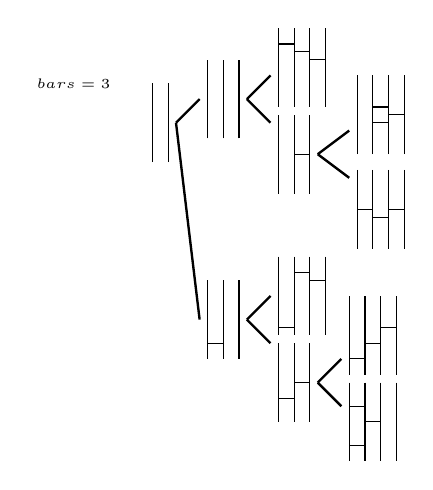
\begin{tikzpicture}
      \node at (-1, 1){\tiny $bars=3$};

        %%L1
           \draw(0, 0) to (0, 1);
           \draw(.2, 0) to (.2, 1);
          
        %%lines 
        \draw[line width = .3mm](.3, .5) to (.6, .8);
        \draw[line width = .3mm](.3, .5) to (.6, -2);
         %% add second line
         
          %L2 
          \draw(.7, .3) to (.7, 1.3);
          \draw(.9, .3) to (.9, 1.3);
          \draw(1.1, .3) to (1.1, 1.3);

        \draw[line width = .3mm](1.2, .8) to (1.5, 1.1);
        \draw[line width = .3mm](1.2, .8) to (1.5, .5);

        %%L3 terminate
        \draw(1.6, .7) to (1.6, 1.7);
          \draw(1.6, 1.5) to (1.8, 1.5);
        \draw(1.8, .7) to (1.8, 1.7);
          \draw(1.8, 1.4) to (2, 1.4);
        \draw(2, .7) to (2, 1.7);
          \draw(2, 1.3) to (2.2, 1.3);
        \draw(2.2, .7) to (2.2, 1.7);

        %%L4 
        \draw(1.6, -.4) to (1.6, .6);
        \draw(1.8, -.4) to (1.8, .6);
          \draw(1.8, .1) to (2, .1);
        \draw(2, -.4) to (2, .6);

        \draw[line width =.3mm](2.1, .1) to (2.5, .4);
        \draw[line width = .3mm](2.1, .1) to (2.5, -.2);

        %%L5 terminate
        \draw(2.6, .1) to (2.6, 1.1);
        \draw(2.8, .1) to (2.8, 1.1);
          \draw(2.8, .5) to (3, .5);
          \draw(2.8, .7) to (3, .7);
        \draw(3, .1) to (3, 1.1);
          \draw(3, .6) to (3.2, .6);
        \draw(3.2, .1) to (3.2, 1.1);

        %%L6 terminate
        \draw(2.6, -.1) to (2.6, -1.1);
          \draw(2.6, -.6) to (2.8, -.6);
        \draw(2.8, -.1) to (2.8, -1.1);
          \draw(2.8, -.7) to (3, -.7);
        \draw(3, -.1) to (3, -1.1);
          \draw(3, -.6) to (3.2, -.6);
        \draw(3.2, -.1) to (3.2, -1.1);

        %%L7 
        \draw(.7, -1.5) to (.7, -2.5);
          \draw(.7, -2.3) to (.9, -2.3);
        \draw(.9, -1.5) to (.9, -2.5);
        \draw(1.1, -1.5) to (1.1, -2.5);
          
          \draw[line width = .3mm](1.2, -2) to (1.5, -1.7);
          \draw[line width = .3mm](1.2, -2) to (1.5, -2.3);
        
      %%L8 terminate
      \draw(1.6, -1.2) to (1.6, -2.2);
        \draw(1.6, -2.1) to (1.8, -2.1);
      \draw(1.8, -1.2) to (1.8, -2.2);
        \draw(1.8, -1.4) to (2, -1.4);
      \draw(2, -1.2) to (2, -2.2);
        \draw(2, -1.5) to (2.2, -1.5);
      \draw(2.2, -1.2) to (2.2, -2.2);
    
      %%L9 
      \draw(1.6, -2.3) to (1.6, -3.3);
        \draw(1.6, -3) to (1.8, -3);
      \draw(1.8, -2.3) to (1.8, -3.3);
        \draw(1.8, -2.8) to (2, -2.8);
      \draw(2, -2.3) to (2, -3.3);

      \draw[line width = .3mm](2.1, -2.8) to (2.4, -2.5);
      \draw[line width = .3mm](2.1, -2.8) to (2.4, -3.1);

      %%L10 terminate
      \draw(2.5, -2.7) to (2.5, -1.7);
        \draw(2.5, -2.5) to (2.7, -2.5);
      \draw(2.7, -2.7) to (2.7, -1.7);
        \draw(2.7, -2.3) to (2.9, -2.3);
      \draw(2.9, -2.7) to (2.9, -1.7);
        \draw(2.9, -2.1) to (3.1, -2.1);
      \draw(3.1, -2.7) to (3.1, -1.7);

      %%L11 terminate
      \draw(2.5, -2.8) to (2.5, -3.8);
        \draw(2.5, -3.6) to (2.7, -3.6);
        \draw(2.5, -3.1) to (2.7, -3.1);
      \draw(2.7, -2.8) to (2.7, -3.8);
        \draw(2.7, -3.3) to (2.9, -3.3);
      \draw(2.9, -2.8) to (2.9, -3.8);
      \draw(3.1, -2.8) to (3.1, -3.8);
    
    \end{tikzpicture}
      
   \end{minipage}\\~\\
  \begin{minipage}{.8\textwidth}
     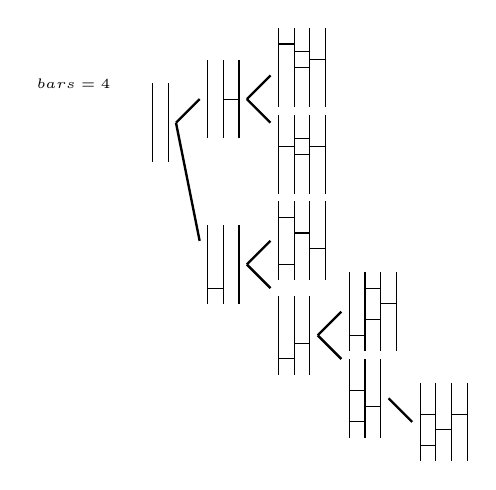
\begin{tikzpicture}
       \node at (-1, 1){\tiny $bars=4$};

      %%L1
      \draw(0, 0) to (0, 1);
      \draw(.2, 0) to (.2, 1);
        \draw[line width = .3mm](.3, .5) to (.6, .8);
        \draw[line width = .3mm](.3, .5) to (.6, -1);
      
        %L2 
          \draw(.7, .3) to (.7, 1.3);
          \draw(.9, .3) to (.9, 1.3);
            \draw(.9, .8) to (1.1, .8);
          \draw(1.1, .3) to (1.1, 1.3);
      
        \draw[line width = .3mm](1.2, .8) to (1.5, 1.1);
        \draw[line width = .3mm](1.2, .8) to (1.5, .5);

        %%L3 terminate
        %%L3 terminate
        \draw(1.6, .7) to (1.6, 1.7);
          \draw(1.6, 1.5) to (1.8, 1.5);
        \draw(1.8, .7) to (1.8, 1.7);
          \draw(1.8, 1.4) to (2, 1.4);
          \draw(1.8, 1.2) to (2, 1.2);
        \draw(2, .7) to (2, 1.7);
          \draw(2, 1.3) to (2.2, 1.3);
        \draw(2.2, .7) to (2.2, 1.7);
        %%L4 termiante
        \draw(1.6, -.4) to (1.6, .6);
          \draw(1.6, .2) to (1.8, .2);
        \draw(1.8, -.4) to (1.8, .6);
          \draw(1.8, .1) to (2, .1);
          \draw(1.8, .3) to (2, .3);
        \draw(2, -.4) to (2, .6);
          \draw(2, .2) to (2.2, .2);
        \draw(2.2, -.4) to (2.2, .6);

        %%L5
        \draw(.7, -.8) to (.7, -1.8);
          \draw(.7, -1.6) to (.9, -1.6);
        \draw(.9, -.8) to (.9, -1.8);
        \draw(1.1, -.8) to (1.1, -1.8);

        \draw[line width=.3mm](1.2, -1.3) to (1.5, -1);
        \draw[line width = .3mm](1.2, -1.3) to (1.5, -1.6);

        %%L6 terminate
        \draw(1.6, -.5) to (1.6, -1.5);
          \draw(1.6, -1.3) to (1.8, -1.3);
          \draw(1.6, -.7) to (1.8, -.7);
        \draw(1.8, -.5) to (1.8, -1.5);
          \draw(1.8, -.9) to (2, -.9);
        \draw(2, -.5) to (2, -1.5);
          \draw(2, -1.1) to (2.2, -1.1);
        \draw(2.2, -.5) to (2.2, -1.5);

        %%L7
        \draw(1.6, -1.7) to (1.6, -2.7);
          \draw(1.6, -2.5) to (1.8, -2.5);
        \draw(1.8, -1.7) to (1.8, -2.7);
          \draw(1.8, -2.3) to (2, -2.3);
        \draw(2, -1.7) to (2, -2.7);

        \draw[line width = .3mm](2.1, -2.2) to (2.4, -1.9);
        \draw[line width = .3mm](2.1, -2.2) to (2.4, -2.5);

        %%L8 terminate
        \draw(2.5, -1.4) to (2.5, -2.4);
          \draw(2.5, -2.2) to (2.7, -2.2);
        \draw(2.7, -1.4) to (2.7, -2.4);
          \draw(2.7, -2) to (2.9, -2);
          \draw(2.7, -1.6) to (2.9, -1.6);
        \draw(2.9, -1.4) to (2.9, -2.4);
          \draw(2.9, -1.8) to (3.1, -1.8);
        \draw(3.1, -1.4) to (3.1, -2.4);

        %%L9
        \draw(2.5, -2.5) to (2.5, -3.5);
          \draw(2.5, -3.3) to (2.7, -3.3);
          \draw(2.5, -2.9) to (2.7, -2.9);
        \draw(2.7, -2.5) to (2.7, -3.5);
          \draw(2.7, -3.1) to (2.9, -3.1);
        \draw(2.9, -2.5) to (2.9, -3.5);

        \draw[line width = .3mm](3, -3) to (3.3, -3.3);
        %%L10 terminate
        \draw(3.4, -2.8) to (3.4, -3.8);
          \draw(3.4, -3.6) to (3.6, -3.6);
          \draw(3.4, -3.2) to (3.6, -3.2);
        \draw(3.6, -2.8) to (3.6, -3.8);
          \draw(3.6, -3.4) to (3.8, -3.4);
        \draw(3.8, -2.8) to (3.8, -3.8);
          \draw(3.8, -3.2) to (4, -3.2);
        \draw(4, -2.8) to (4, -3.8);

    
      \end{tikzpicture}\hspace{10mm}
      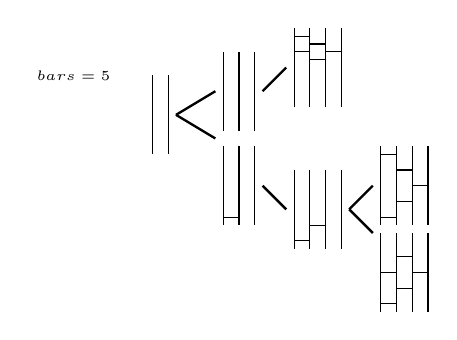
\begin{tikzpicture}
            \node at(-1, 5){\tiny $bars=5$};
       %     %%L1
            \draw(0, 4) to (0, 5);
            \draw(.2, 4) to (0.2, 5);
           
            \draw[line width = .3mm](.3, 4.5) to (0.8, 4.8);
            \draw[line width =.3mm](.3, 4.5) to (.8, 4.2);
 
       %     %%L2
 
            \draw(.9, 4.3) to (.9, 5.3);
            \draw(1.1, 4.3) to (1.1, 5.3);
            \draw(1.3, 4.3) to (1.3, 5.3);
 
            %L3 terminate
            \draw[line width = .3mm](1.4, 4.8) to (1.7, 5.1);
             \draw(1.8, 4.6) to (1.8, 5.6);
               \draw(1.8, 5.3) to (2, 5.3);
              \draw(1.8, 5.5) to (2, 5.5);
             \draw(2, 4.6) to (2, 5.6);
               \draw(2, 5.4) to (2.2, 5.4);
               \draw(2, 5.2) to (2.2, 5.2);
             \draw(2.2, 4.6) to (2.2, 5.6);
               \draw(2.4, 5.3) to (2.2, 5.3);
             \draw(2.4, 4.6) to (2.4, 5.6);
 
      %       %%L4 
             \draw(.9, 4.1) to (.9, 3.1);
               \draw(.9, 3.2) to (1.1, 3.2);
             \draw(1.1, 4.1) to (1.1, 3.1);
             \draw(1.3, 4.1) to (1.3, 3.1);
 
            \draw[line width = .3mm](1.4, 3.6) to (1.7, 3.3);
      %  %      %%L5
             \draw(1.8, 3.8) to (1.8, 2.8);
               \draw(1.8, 2.9) to (2, 2.9);
             \draw(2, 3.8) to (2, 2.8);
               \draw(2, 3.1) to (2.2, 3.1);
             \draw(2.2, 3.8) to (2.2, 2.8);
             \draw(2.4, 3.8) to (2.4, 2.8);
 
            \draw[line width = .3mm](2.5, 3.3) to (2.8, 3);
            \draw[line width = .3mm](2.5, 3.3) to (2.8, 3.6);
       %     %%L6 terminate
            \draw(2.9, 3.1) to (2.9, 4.1);
              \draw(2.9, 3.2) to (3.1, 3.2);
              \draw(2.9, 4) to (3.1, 4);
            \draw(3.1, 3.1) to (3.1, 4.1);
              \draw(3.1, 3.4) to (3.3, 3.4);
              \draw(3.1,3.8) to (3.3, 3.8);
            \draw(3.3, 3.1) to (3.3, 4.1);
              \draw(3.3, 3.6) to (3.5, 3.6);
            \draw(3.5, 3.1) to (3.5, 4.1);
       %     %%L7 terminate
            \draw(2.9, 3) to (2.9, 2);
               \draw(2.9, 2.1) to (3.1, 2.1);
               \draw(2.9, 2.5) to (3.1, 2.5);
            \draw(3.1, 2) to (3.1, 3);
               \draw(3.1, 2.3) to (3.3, 2.3);
               \draw(3.1, 2.7) to (3.3, 2.7);
            \draw(3.3, 2) to (3.3, 3);
               \draw(3.3, 2.5) to (3.5, 2.5);
            \draw(3.5, 2) to (3.5, 3);
        \end{tikzpicture}
   \end{minipage}\\~\\
   \begin{minipage}{.8\textwidth}
    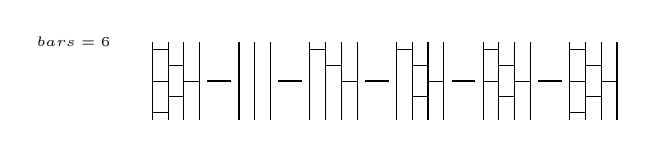
\begin{tikzpicture}
      \draw node at (-1, 1){\tiny $bars=6$};
      \draw(0, 0) to (0, 1);
        \draw(0, .1) to (.2, .1);
        \draw(0, .5) to (.2, .5);
        \draw(0, .9) to (.2, .9);
      \draw(.2, 0) to (.2, 1);
        \draw(.2, .3) to (.4, .3);
        \draw(.2, .7) to (.4, .7);
      \draw(.4, 0) to (.4, 1);
        \draw(.4, .5) to (.6, .5);
      \draw(.6, 0) to (.6, 1);

      \draw[line width = .3mm](.7, .5) to (1, .5);
      %%L2
      \draw(1.1, 0) to (1.1, 1);
      \draw(1.3, 0) to (1.3, 1);
      \draw(1.5, 0) to (1.5, 1);

      \draw[line width = .3mm](1.6, .5) to (1.9, .5);

      %%L3
      \draw(2, 0) to (2, 1);
        \draw(2, .9) to (2.2, .9);
      \draw(2.2, 0) to (2.2, 1);
        \draw(2.2, .7) to (2.4, .7);
      \draw(2.4, 0) to (2.4, 1);
        \draw(2.4, .5) to (2.6, .5);
      \draw(2.6, 0) to (2.6, 1);
    
      \draw[line width=.3mm](2.7, .5) to (3, .5);

      %L4
      \draw(3.1, 0) to (3.1, 1);
        \draw(3.1, .9) to (3.3, .9);
      \draw(3.3, 0) to (3.3, 1);
        \draw(3.3, .7) to (3.5, .7);
        \draw(3.3, .3) to (3.5, .3);
      \draw(3.5, 0) to (3.5, 1);
        \draw(3.5, .5) to (3.7, .5);
      \draw(3.7, 0) to (3.7, 1);

      \draw[line width = .3mm](3.8, .5) to (4.1, .5);

      %L5
      \draw(4.2, 0) to (4.2, 1);
        \draw(4.2, .9) to (4.4, .9);
        \draw(4.2, .5) to (4.4, .5);
      \draw(4.4, 0) to (4.4, 1);
        \draw(4.4, .7) to (4.6, .7);
        \draw(4.4, .3) to (4.6, .3);
      \draw(4.6, 0) to (4.6, 1);
        \draw(4.6, .5) to (4.8, .5);
      \draw(4.8, 0) to (4.8, 1);
    
      %%L6 terminate
      \draw[line width = .3mm](4.9, .5) to (5.2, .5);
      \draw(5.3, 0)  to (5.3, 1);
        \draw(5.3, .9) to (5.5, .9);
        \draw(5.3, .5) to (5.5, .5);
        \draw(5.3, .1) to (5.5, .1);
      \draw(5.5, 0)  to (5.5, 1);
        \draw(5.5, .7) to (5.7, .7);
        \draw(5.5, .3) to (5.7, .3);
      \draw(5.7, 0)  to (5.7, 1);
        \draw(5.7, .5) to (5.9, .5);
      \draw(5.9, 0)  to (5.9, 1);
    \end{tikzpicture}
    
   \end{minipage}
  \caption{The forest for all ladders in $CanL\{\pi_{4}\}$ generated by the Cyclic Inversion Algorithm. The first tree has all ladders with zero bars, the second tree 
  has all ladders with 1 bar, etc. }
\end{figure}\pagebreak

It has been stated that the forest created by the Cyclic Inversion algorithm generates $CanL\{\pi_{N}\}$. This claim has 
yet to have been proven, so the following lemma will prove this claim.

\begin{lemma}
  The forest created by the Cyclic Inversion algorithm generates $CanL\{\pi_{N}\}$
\end{lemma}
\begin{proof}
  The proof is done by way of contradiction. Suppose that the cyclic inversion algorithm generated $N!$ ladders and did not generate $CanL\{\pi_{N}\}$, 
  then there would be two or more ladders generated by the cyclic inversion algorithm which belonged to the same $OptL\{\pi_{N}\}$. If that were the 
  case, then at least one of these ladders would not be the root ladder from the $OptL\{\pi_{N}\}$. However, it was already stated that the canonical 
  representative for $CanL\{\pi_{N}\}$ was the root ladder from each $OptL\{\pi_{N}\}$, which leads to a contradiction. Therefore each ladder generated 
  by the cyclic inversion algorithm is part of $CanL\{\pi_{N}\}$. 
\end{proof}

For each tree in the forest, the algorithm effectively relocates one or more bars from the $Kth$ route to the the $K-1th$ route 
until the $K-1th$ route has either no more space left for bars, i.e. the $K-1th$ route has $K-2$ bars in the ladder or the number of 
bars in the ladder is equal to the current limit. This is what is happening when 
a bar is added to some route; it only gets added once the bar of a greater route has been removed unless the route is $K=N$. When $K=N$, 
bars are continuously added to the $K=Nth$ route until no more bars can be added for $K=N$ or the number of bars is equal to the current limit. 
For example, suppose $N=5$ and the current limit for the number of bars is three, then when $K=N$, the first ladder for this forest will 
be the ladder in which all three bars belong to the fifth route. Seeing as element $5$ has at most four bars in the ladder. However, 
if the current limit is 6, then the first ladder in the forest will have all the bars belonging to the fifth root as well as the first two bars 
belonging to the fourth root, seeing as the $5th$ element has at most $4$ bars, yet the given current limit for the number of bars is six. Once 
all the bars for the $K=Nth$ route have been added, the upper leftmost bar of the $K=Nth$ route is relocated to the $N-1th$ route, this process 
continues until the $N-1th$ route has had all of its bars added. Upon completion, all the bars are removed from the $N-1th$ route, and the 
first bar of the $N-2th$ route is added. Then the algorithm repeats itself by adding all the bars to the $K=Nth$ route until the current limit 
is reached or the $Nth$ route has $N-1$ bars added to the ladder. Again, the upper left most bar 
of the $K=Nth$ route is relocated to the $N-1th$ route; this continues until the number of bars added is equal to the current limit or 
the $N-1th$ route has $N-2$ bars added, keeping in mind that the $N-2th$ route now has a bar in the ladder. Once complete, all the bars of the 
$N-1th$ route are removed, and the next bar of the $N-2th$ route is added if possible or all the bars of the $N-2th$ route are removed, and the 
first bar of the $N-3rd$ route is added. The forest terminates when the number of bars in the ladder is equal to the current limit and 
each bar in the ladder belongs to the smallest route(s). For example, if $N=4$ and the current limit for the number of bars is three, then 
the ladder which terminates the forest for $CurrentLimit=3$ is the ladder with one bar belonging to route $2$ and two bars belonging to route 
$3$. It must be noted that the row and column calculation for the insertion of a bar is the same as the SJT algorithm which is why the proofs 
for the row and column calculation are not provided for the Cyclic Inversion algorithm. 



\subsection{Results}
    In the results section, the runtimes of the two algorithms will be provided. The run times are done without printing the ladders. When the ladders are printed, the runtime increases by a substantial amount. 
    The runtime for each algorithm for $N=10$ will be provided in a table. In the analysis section, the table will be further analyzed along with 
    the time and space complexity for each algorithm.
\begin{table}
    \begin{tabular}{ |p{3cm}||p{3cm}|p{3cm}|}
        \hline
        \multicolumn{3}{|c|}{Runtimes for generating $CanL\{\pi_{N}\}$ in seconds} \\
        \hline
            $N$ value& Cyclic Inversion & Modified SJT\\
        \hline
            1   & 0.000000    &0.000000\\
            \hline
            2 &   0.000000  & 0.000000\\

            \hline
            3 &0.000000 & 0.000000\\
            \hline
            4 &0.000000 & 0.000000\\
            \hline
            5 &   0.000000  & 0.000000\\
            \hline
            6 & 0.000000  & 0.000000  \\
            \hline
            7 & 0.000000  & 0.000000\\
            \hline
            8 & 0.000000 & 0.000000\\
            \hline
            9 & 0.093750 & 0.000000\\
            \hline
            10 & 0.968750 & 0.031250\\
            \hline

            11 & 12.718750 & 0.250000\\
            \hline 
            12 & 174.312500 & 2.781250\\
        \hline
\end{tabular}
    \caption{The table with the runtimes for listing $CanL\{\pi_{N}\}$ using the Cyclic Inversion Algorithm and Modified SJT Algorithm.}
\end{table}

\section{Analysis}
\subsection{Introduction}
    From looking at the table in the results section, it is cear that the modified SJT algorithm performs 
    better than the Cyclic Inversion algorithm. The reson(s) for this disparity in performance 
    will be analyzed. Following this analysis, areas of application and practical relavence for the Listing Problem 
    will be discussed along with concluding remarks.

\subsection{Performane Analysis}
    As $N \geq 9$ there is a noticeable difference between the runtimes of the two algorithms by a sizable order 
    of magnitude. Cleary the modified SJT algorithm performs better than the Cyclic Inversion algorithm. The reason(s) 
    for this improved performance are the following. Firstly, the time complexity of the two algorithms are different. 
    The time complexity for the modified SJT algorithm is $(N!)N$. The time will be proven in the following lemma.
    \begin{lemma}
        The time complexity for the modified SJT algorithm is $O((N!)N)$
    \end{lemma}
    \begin{proof}
        The $N!$ factor is fairly straightforward, the algorithm creates all $N!$ ladders in $CanL\{\pi_{N}\}$ which 
        accounts for the $N!$ factor. The $N$ factor is a result of the second for loop found in the algorithm. The first for loop 
        fount in the modified sjt function runs $(N-1)$ times each time the modified SJT function is called, however on each 
        iteration of this for loop a ladder is listed, therefore the runtime of this for loop is accounted for by the $N!$ factor. However, 
        the second for loop in the helper SJT function runs at worst, $N-1$ times before listing a ladder. This worst case 
        is when the $K=2$ route needs to have a bar inserted or removed. Therefore, this second for-loop accounts for the $N$ factor 
        in the time complexity. Thus, the time complexity of the modified SJT algorithm is $O((N!)N)$.
    \end{proof}

    On the other hand, the time complexity of the Cyclic Inversion algoirthm is $O((N!)N^{2})$. The time complexity for the Cyclic 
    Inversion Algorithm will be proven in the following lemma.

    \begin{lemma}
        The time complexity for the Cyclic Inversion algorithm is $O((N!)N^{2})$
    \end{lemma}
    \begin{proof}
        The $N!$ factor is fairly straightforward, the algorithm creates all $N!$ ladders in $CanL\{\pi_{N}\}$ which accounts 
        for the $N!$ factor. The $N^{2}$ factor is a result of the for loop that is executed when $2 \leq K < N$. This for loop runs 
        from $1$ to $K$ for each value of $K$. Thus, the for loop is executed $1 + 2 + 3 + 4, ... + N-1$ times. This summation 
        is equal to $((N-1)N-2)/2$ which is reduced to $N^{2}$. Therefore the for-loop when $2 \leq K < N$ accounts for the $N^{2}$
        factor.
    \end{proof}

    \subsection{Application(s)}
    The applications for generating $CanL\{\pi_{N}\}$ are currently unknown insofar as this problem has yet to be solved to my knowledge. 
    However, if I am to be granted some speculation, I could provide some hypothetical scenarios in which listing $CanL\{\pi_{N}\}$ could 
    be of interest. The first hypothetical application could be to model an \emph{oblivious sorting system} for $N!$ permutations. An oblivious 
    sorting system is a system such that the sorting operations are done irrespective of the data being passed to the system. Recall 
    that a bar in a ladder simply swaps two adjacent elements in a permutation. Due to the static nature of each ladder, the swap operation 
    resulting from two elements in a permutation crossing a bar is unchanging. 
    Seeing as each ladder in $CanL\{\pi_{N}\}$ sorts the corresponding permutation of order $N$, one can implement all of $CanL\{\pi_{N}\}$ 
    for some arbitrary $N$ value and then pass each permutation of order $N$ through its respective ladder from $CanL\{pi_{N}\}$ thus 
    resulting in each permutation being ordered. The ladders from $CanL\{\pi_{N}\}$ only need to be generated once and saved. Once this is done 
    a permutation can be passed to the correct ladder and it can be sorted by having each of its elements pass through the ladder. 

\chapter{The Minimum Height Problem}
\label{chapter:minheightproblem}
\subsection{Introduction to the Problem}
Listing problems are common problems in cambinatorics. In general, listing problems 
focus on enumerating the objects of a given finite set in some specific order. The listing problem in this thesis 
will be termed \emph{The Canonical Ladder Listing Problem}. The problem is stated as follows: Let $\pi_{N}$ be one of $N!$ arbitrary permutation of $[1 \dots N]$. 
Let \emph{The Canonical Ladder} be a unique ladder from $OptL\{\pi_{N}\}$. Let $CanL{\pi_{N}}$ be the set of all canonical ladders for 
all $N!$ permutations of order $N$. Let $L_{i}$ be the canonical ladder of some arbitrary permuation $OptL\{\pi_{N_{i}}\}$. A \emph{change} is defined as the insertion or 
deletion of one or more bar(s) to get from $L_{i}$ to $L{i+1}$, or the relocation of one or more bars in $L_{i}$ to get to $L_{i+1}$. The relocation of a bar 
is defined as moving a bar from a given row and column, to a new row and column in the ladder. The \emph{Listing Problem} asks given all permutations of 
order $N$, is there a way to generate the canonical ladder from each $OptL\{\pi_{N}\}$. 
Furthermore, if there is a way to do so, what is the most efficient way to do so. Efficiency is defined as 
using minimal change to transition from $L_{i}$ to $L_{i+1}$. For example, let $N=4$, there are $N!$ or 24 permutations 
of order $N$. $|CanL{\pi_{N}}=24|$; therefore there are 24 canonical ladders, one from each $OptL\{\pi_{4}\}$. Is there a way to generate 
all 24 canonical ladders for each $OptL\{\pi_{N}\}$? Furthermore, if there is such a way, what is the most efficient way 
to do so; i.e. the algorithm that requires the minimal amount of change to get from $L_{i}$ to $L_{i+1}$. See Table -- for 
the 24 permutations of order 4.
\begin{table}[]
    \begin{center}
       \begin{tabular}{|c |c |c |c |}
        \hline
        1234 & 1243 & 1324 & 1342 \\ \hline
        1423 & 1432 & 2143 & 2134 \\ \hline 
        2314 & 2341 & 2413 & 2431 \\ \hline 
        3124 & 3142 & 3214 & 3241 \\ \hline 
        3412 & 3421 & 4123 & 4132 \\ \hline 
        4213 & 4231 & 4312 & 4321 \\ \hline 
        
    \end{tabular}
    \caption{Table for all 4!, 24, permutations of order 4} 
    \end{center}

 \end{table}



Each of these permutations has one or more ladders in each of their respective 
$OptL\{\pi\}$. The canonical ladder listing  problem asks, given some arbitrary $N \geq 1$,
what is the most efficient way to list $CanL\{\pi_{N}\}$. Recall that in order to get from $L_{i}$ to $L_{i+1}$, at least one of the 
two changes must be applied to $L_{i}$ to get to $L_{i+1}$. At least one bar has to be removed/added or at least one bar 
has to be reolocated in $L_{i}$ to get to $L_{i+1}$.

\begin{theorem}
    In order to transition from canonical ladder $L_{i}$ to canonical ladder $L_{i+1}$, at least one bar has to be added or 
    removed from $L_{i}$ or at least one bar has to be relocated in $L_{i}$.
\end{theorem}
\begin{proof}
    We begin this proof by contradiction. Suppose $L_{i}$ is some arbitrary canonical ladder for permutation of 
    order $N$. Suppose that $L_{i+1}$ is the next canonical ladder in the set of canonical ladders. Each canonical 
    ladder represents a network of adjacent transposisitions of the corresponding permutations, $\pi_{i}$ and 
    $\pi_{i+1}$ used to sort $\pi_{i}$ and $\pi_{i+1}$ respectively. $\pi_{i}$ and $\pi_{i+1}$ are unique. Let $Inv{\pi}$ 
    be the set of all inversions is $\pi$. Let $AdjInv{\pi} \subset Inv{\pi}$ be a subset of inversions in $\pi$
    that are adjacent. A bar in $L_{i}$ and $L_{i+1}$ uninverts an adjacent inversion in from $AdjInv{\pi_{i}}$ and $AdjInv{\pi_{i+1}}$ respectively. 
    Note, that when an adjacent inversion is uninverted, a new intermediate permuation is derived from $\pi$. Let $IntPi(\pi)$
    be the permutation of intermediate permutations, beginning with $\pi$ that result from performing adjacent transpositions on $AdjInv{\pi}$, terminating with 
    the sorted permutation. The row in the ladder represents the order of uninverting adjacent transpositions in some intermediate permutation in $IntPi(\pi)$.
    For example, row 1 in $L_{i}$ represents uninverting adjacent inversions in $\pi_{i}$. The result of uninverting these 
    adjacent inversions is the second intermediate permutation in $IntPi(\pi)$, $\pi'$. Row two represents uninverting the adjecent 
    inversions in $\pi'$ resulting in $\pi''$, etc. If no bars are added or removed from $L_{i}$ then 
    the number of bars in $L_{i+1}$ is the same as in $L_{i}$. This means that the number of adjacent inversions that are uninverted 
    in $\pi_{i}$ is the same as in $\pi_{i+1}$. Next, suppose that no bars are relocated in $L_{i}$ to get to $L_{i+1}$. This would 
    mean that the same adjacent inversions in $\pi_{i}$ exist in $\pi_{i+1}$ and furthermore, the order in which these adjacent 
    iversions were uninverted would be the same for $\pi_{i}$ and $\pi_{i+1}$; in other words the $IntPi(\pi_{i})=IntPi(\pi_{i+1})$ But this is a contradiction, 
    seeing as $pi_{i}$ and $pi_{i+1}$ are unique. Therefore, at least one 
    bar has to be added or removed from $L_{i}$ to get to $L_{i+1}$ or at least one bar in $L_{i}$ has to be relocated to get to $L_{i+1}$.
    See fig- for an example of $L_{3 1 4 2}$ with the corresponding $IntPi(3 1 4 2)$.
\end{proof}

\begin{figure}[!htp]
    \begin{center}
    \begin{tikzpicture}
        %%draw the lines
        \draw(0, 0) to (0, 4);
            \node at(0, 4.3){3};
            \node at(0, -0.3){1};
        \draw(2, 0) to (2, 4);
            \node at(2, 4.3){1};
            \node at(2, -0.3){2};
        \draw(4, 0) to (4,4);
            \node at(4, 4.3){4};
            \node at(4, -0.3){3};
        \draw(6, 0) to (6, 4);
            \node at(6, 4.3){2};
            \node at(6, -0.3){4};
        \node at(8, 3){3,1,4,2};
        \node at(8, 2){1,3,2,4};
        

        \node at(-2, 4.3){$R_{0}$};
        \node at(-2, 3){$R_{1}$};
        \node at(-2, 2){$R_{2}$};
        \node at(-2, -0.3){$R_{3}$};

        %%draw the bars
        \draw(0, 3) to (2, 3);
        \draw(2, 2) to (4, 2);
        \draw(4, 3) to (6,3);

    \end{tikzpicture}
    \end{center}
    \caption{The rows are on the left of the ladder designating the order in which the adjacent inversions will be uninverted.
    On the right is the $IntPi(3,1,4,2)$ that results from the ladder univerting  the adjacent inversions in 3,1,4,2 in the order 
    of the rows. $IntPi(3,1,4,2)=((3,1,4,2), (1,3,2,4), (1,2,3,4))$}
\end{figure}

In this thesis, two listing algorithms were used to generate the canonical 
ladders for each $OptL\{\pi_{N}\}$. The first of these listing algorithms 
is a modification of the Steinhaus-Johnson-Trotter permutation listing algorithm. 
The second listing algorithm is, as far as I know, a novel algorithm. 
It is termed the cyclic-inversion algorithm. Both of these algorithms will 
be described, explained and analyzed throughout the remainder of the chapter.\par

Before proceeding, the justification for the canonical ladder will be presented. 
The canonical ladder is selected as the root ladder from each $OptL\{\pi_{N}\}$. 
The rationale for always choosing the root ladder was due to the fact that every 
permutation has a root ladder in its $OptL\{\pi\}$ whereas not every permutation 
has a non-root ladder. For example, given the permutation $(2,1,4,3)$, $OptL\{(2,1,4,3)\}$
has only one ladder which is the root ladder. This is because there are only two 
bars in the ladder, thus there is no swap operation that can be performed.
\begin{theorem}
    If $|OptL\{\pi\}|=1$ then the ladder is the root ladder.
\end{theorem} 
\begin{proof}
    The root ladder is defined as the ladder whose clean level is one.
    This means either there is no bar of a lesser element above the route a 
    greater element. Keeping in mind that the clean level of the root ladder is one, next consider what is meant by a  \emph{child bar}
     which is a bar to the bottom left or right of a given bar $x$. Within the context of the root ladder, 
     if the left endpoint of the child bar is directly below the right end point of $x$ then the child is a 
    right child of $x$. If the right end point of the child bar is directly 
    below the left end point of $x$ then it is a left child. 
    Keeping in mind the root ladder has not undergone any right swap operations, then
    if a child is a right child 
    then the child belongs to the same route of $x$ in the root ladder. 
    Let $R_{m}$ denote this route. Let $x$ be a bar representing an inversion with element $m$ and $k$.
    The right child of $x$ is a bar which represents an inversion 
    with $m$ and some element to the right of $k$. Suppose this was not the case, 
    then this would mean that the right child of $x$ was either a bar representing an inversion 
    between some element $m'$ that was greater than $m$ or lesser than $m$. If $m'$ was 
    greater than $m$ then this would be a contradiction seeing as $x$ would be above the bar of a route 
    of a greater element which contradicts the definition of the root ladder. On the other hand if 
    $m'$ were lesser than $m$, then $m$ would form an inversion with $m'$ and therefore 
    the bar representing this inversion would be part of the route of $m$ route. Thus, the right child 
    of a bar $x$ belongs to the same route as $x$ in the root ladder.\par The left child of $x$
    represents an inversion with some lesser element than $m$ and $k$. Suppose this was not the case, 
    then the left child could belong to a route greater than $m$, but if that were the case, this contradicts 
    the definition of the root ladder.
    Thus the first element of the left child must belong to the route of some lesser element than $m$. Next suppose that 
    the lesser element of the left child of $x$ was not $k$. Let this element be termed $k'$.
    $k'$ forms an inversion with the greater element of the left child of $x$. But since the greater element of the left child is less than $m$, 
    then $m$ would also form an inversion with $k'$. Thus, the bar of $m$ and $k'$ would be the parent of the left child, which is also 
    a contradiction, seeing as the left child is the child of bar $x$. Therefore the left child of $x$ must be a bar that 
    it belongs to the route of a lesser element than $m$ and its lesser element is $k$.\par 
    Please refer to FIG--- to view an example of a root ladder with left and right children.\pagebreak

    
\end{proof}


\begin{figure}[!htp]
    \begin{center}
    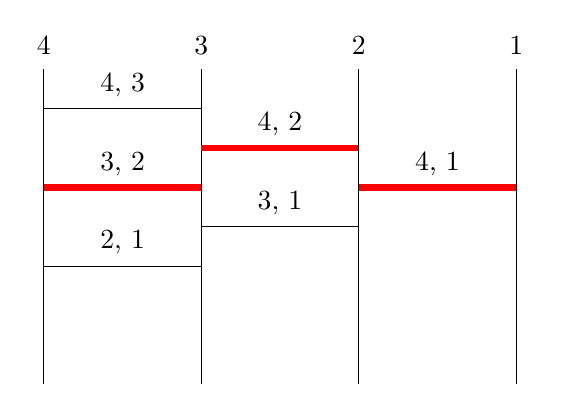
\begin{tikzpicture}
        \draw(0, 0) to (0, 4);
            \node at(0, 4.3){4};
             \draw(0, 3.5) to (2, 3.5);
                \node at(1, 3.8){4, 3};
            
            \draw[line width=0.8mm, red](0, 2.5) to (2, 2.5);
                \node at(1, 2.8){3, 2};

            \draw(0, 1.5) to (2, 1.5);
                \node at(1, 1.8){2, 1};
        \draw(2, 0) to (2, 4);
            \node at(2, 4.3){3};
                \draw[line width=.8mm, red](2, 3) to (4, 3);
                    \node at(3, 3.3){4, 2};
           
                \draw(2, 2) to (4, 2);
                    \node at(3, 2.3){3, 1};
        \draw(4, 0) to (4, 4);
             \node at(4, 4.3){2};
                \draw[line width=0.8mm, red](4, 2.5) to (6, 2.5);
                    \node at (5, 2.8){4, 1};
        \draw(6, 0) to (6, 4);
            \node at(6, 4.3){1};


    \end{tikzpicture}
    \end{center}
    \caption{The root ladder of $(4,3,2,1)$. Note that bar 4,2 is the parent of bar 3,2 and 4,1. Also note that 
    bar 3, 2 is the the left child of 4, 2 and 4, 1 is the right child.}
\end{figure}



\section{Procedure}

Thus far, the problem has been introduced and the required terminologt has been defined. Recall that there are two 
changes; the insertion/deletion of bars or repositioning bars.
However, there has yet to be discussion regarding the two 
listing algorithms. In the procedure section 
we look at each of the algorithms and explain what 
each of the algorithms are doing. The goal is to transition from 
$L_{i}$ to $L_{i+1}$ in $CanL{\pi_{N}}$ with minimal change, which means adding or removing 
the least number of bars to get from $L_{i}$ to $L_{i+1}$ or relocating 
the least number of bars to get from $L_{i}$ to $L_{i+1}$.\par 

The reason that the modified SJT and CI algorithms were chosen is because they allow 
for minimal change from $L_{i}$ to $L_{i+1}$. While conducting this research, modifications 
to the permutation listing algorithms mentioned in chapter one were applied. Recall that 
these listing algorithms were Zaks, Heaps, and Lexicographic. These listing algorithms 
did not allow for minimal change when transitioning from $L_{i}$ to $L_{i+1}$.
%%section SJT
\subsection{Steinhaus-Johnson-Trotter}
\begin{algorithm}
  \caption{Modified SJT algorithm for processing at $K=N$}
  \begin{algorithmic}[1]
    \Function{modifiedSjt}{$N$, $Ladder[2(N-1)-1][N-1]$, $Arr[N-1]$, $Direction[N]$}


      \State $print(Ladder)$

      %%base case
      \If{$globalCount = N!$}
        \State return
      \EndIf

     
      \State $dir \gets direction[N]$
      \State $K \gets N-1$
      %%swap the nth element n-1 times
      \For{$i \gets 1$,$i < N$, $i \gets i+1$}
        
        \If{$dir = left$}
            \State $row \gets (N) - i$
            \State $col \gets row$
            \State $ladder[row][col] \gets 1$
        \Else
            \State $row \gets i$
            \State $col \gets row$
            \State $ladder[row][col] \gets 0$
        \EndIf
        \State $globalCount \gets globalCount+1$
        \State $print(Ladder)$

      \EndFor
      \State $direction[N] \gets !direction[N]$
      \State $HELPERSJT(K, N, ladder, arr, direction)$
      \State $MODIFIEDSJT(N,  ladder, arr, direction)$

    \EndFunction
  \end{algorithmic}
\end{algorithm}

%%helper algorithm
\begin{algorithm}
  \caption{Helper SJT algorithm for processing when $2 \leq K < N$}
  \begin{algorithmic}[1]
    \Function{helpersjt}{$N$, $K=(N-1)$, $Ladder[2(N-1)-1][N-1]$, $Arr[N-1]$, $Direction[N]$}

      \For{$i \gets K$, $i \geq 1$, $i \gets i-1$}
        \If{$arr[K] < K$}
        \State $globalCount \gets globalCount + 1$

          \If{$dir[K] = LEFT$}
            \State $row \gets (N-1) + (N-K) - arr[K]$
            \State $col \gets (K) - arr[K]$
            \State $ladder[row][col] \gets 1$

          \Else
            \State $row \gets  (N-1) + (N-K) + arr[K] - (K-2)$
            \State $col \gets arr[K]$
            \State $ladder[row][col] \gets 0$
          \EndIf
          \State $arr[K]\gets arr[K]+1$
          \State return
        \Else 
          \State $arr[K] \gets 0$
          \State $direction[K] \gets !direction[K]$
        \EndIf
        $K \gets K-1$
      \EndFor
      \EndFunction
  \end{algorithmic}
\end{algorithm}
\pagebreak

Let the \emph{identity ladder} be the ladder for the sorted permutation from $[1 \dots N]$.
Let the initial conditions of the algorithm be the fallowing. The $Ladder= 2D array$,  
let $n \geq 1$, let $arr$ be set to zero for all indexes. Let $dir$ be set to false 
for all indexes. The principles of the algorithm are the following, if the direction for a 
given route is false, then bars will be added for that given route, from right to left, bottom to top, until no more bars can be added. Let a 
$1$ at $Ladder[row][col]$ indicate a bar has been added to the ladder at the given row and column.
If the direction for a given route is true, then bars will be removed for that given route, left to right, top to bottom, until 
no more bars can be removed. Let a $0$ at $Ladder[row][col]$ indicate a bar has been removed from the ladder 
at the given row and column. Let $K$ be the value of some given route where $1 < K <= N$. Note that element one has no route.
The number of bars for a given route is $1 \leq K < N$. This is because the maximum number of inversions 
the $kth$ element can make is $K-1$, therefore the $kth$ route can have at most $N-1$, if $K=N$, and 
at least $1$ bar if $K=2$. Once all the bars for the $Kth$ route have been added 
or removed, the direction for the $Kth$ route is switched, indicating that its bars will be removed if they 
were added, or added if they were removed. Once all the bars for the $Kth$ route have been added or removed, 
the next bar of the $K-1th$ route will be added or removed. Once this is done, the bars of route $K$ will 
then be added if they were previously removed or removed if previously added. Repeat this process until all
$N!$ ladders have been generated.


%%prove the dimensions of the datastructure
\begin{theorem}
  The number of rows required for the ladder data-structure is $2(N-1) - 1$ and the number of columns required for 
  the ladder is $N-1$.
\end{theorem}
\begin{proof}
  The number of columns is fairly straighforward. Seeing as there are always $N$ elements in $\pi_{N}$, 
  a column represents a gap between lines in the corresponding ladder-lottery. Let $Line_{i}$ be a vertical line in a ladder-lottery 
  with some element in $\pi_{N}$ at the top of the line and the $ith$ element in $\pi_{N}$ be 
  at the bottom of $Line_{i}$. There are $N$ lines in the ladder-lottery, a column in the ladder data-structure
  simply represents a gap between two adjacent lines in the ladder lottery.\par 
  The number of rows for the ladder data-structure is calculated a follows, given $\pi_{N}$, the minimal 
  number of rows required is when $\pi_{N}$ is sorted. In this case there are zero rows because there are 
  zero bars added to the ladder. This ladder is $L_{N_{ID}}$ and is 
  the first ladder in $CanL{\pi_{N}}$. When a bar is added to the ladder it can be added to an already existing row 
  or to a new row. If the current state of the ladder is $L_{N_{ID}}$ then the new bar will create the $N-1$th row in the 
  $N-1$th column. Let the bar belong to the $Nth$ route, then repeat adding bars for the $Nth$ route, bottom to top left to right. 
  Since no two bars of the $Nth$ route can be on the same row, this will require $N-1$ rows. Note, if they were added to the same 
  row, then the left end point of the right bar would be touching the right end point of the left bar which is disallowed. Once the 
  bars of the $Nth$ element are added, the bars of the $N-1th$ route will be added. The $N-1th's$ first bar 
  will be added to the $N-2$ column, otherwise it would be directly below the first bar of the $Nth$ route, which is a violation. 
  Since the first bar of the $N-1$'s element is added to column $N-2$, then it must be given a new row, otherwise its right end point 
  will be touching  the left end point of the first bar of route $N$. The remaining $N-2$ bars of element $N-1$
  will be added bottom right to top left, but none of their end points will touch the end points of element $N$ seeing as they will 
  always be two columns apart from any bar in $N's$ route. The same logic applies to element $N-2$, it will require one extra row for its 
  first bar, in order not to touch the first bar of element $N-1$, but the remainder of its bars will always be two columns away from 
  the remainder of the bars for $N-1$, etc. Therefore there are $N-2$ rows required for each element, $K$,  $2 \leq K < N$. Note that element 
  $1$ has no bars in its route. Therefore there are $(N-1)$ rows required for element $N's$ route plus $(N-2)$ rows required for 
  elements $2 \leq K < N$. In conclusion the number of rows required is $(N-1) + (N-2) = 2(N-1)-1$. See figure for the tree of ladders 
  generated by modified SJT for $N=4$
\end{proof}



\begin{figure}[!htp]
\begin{center}
  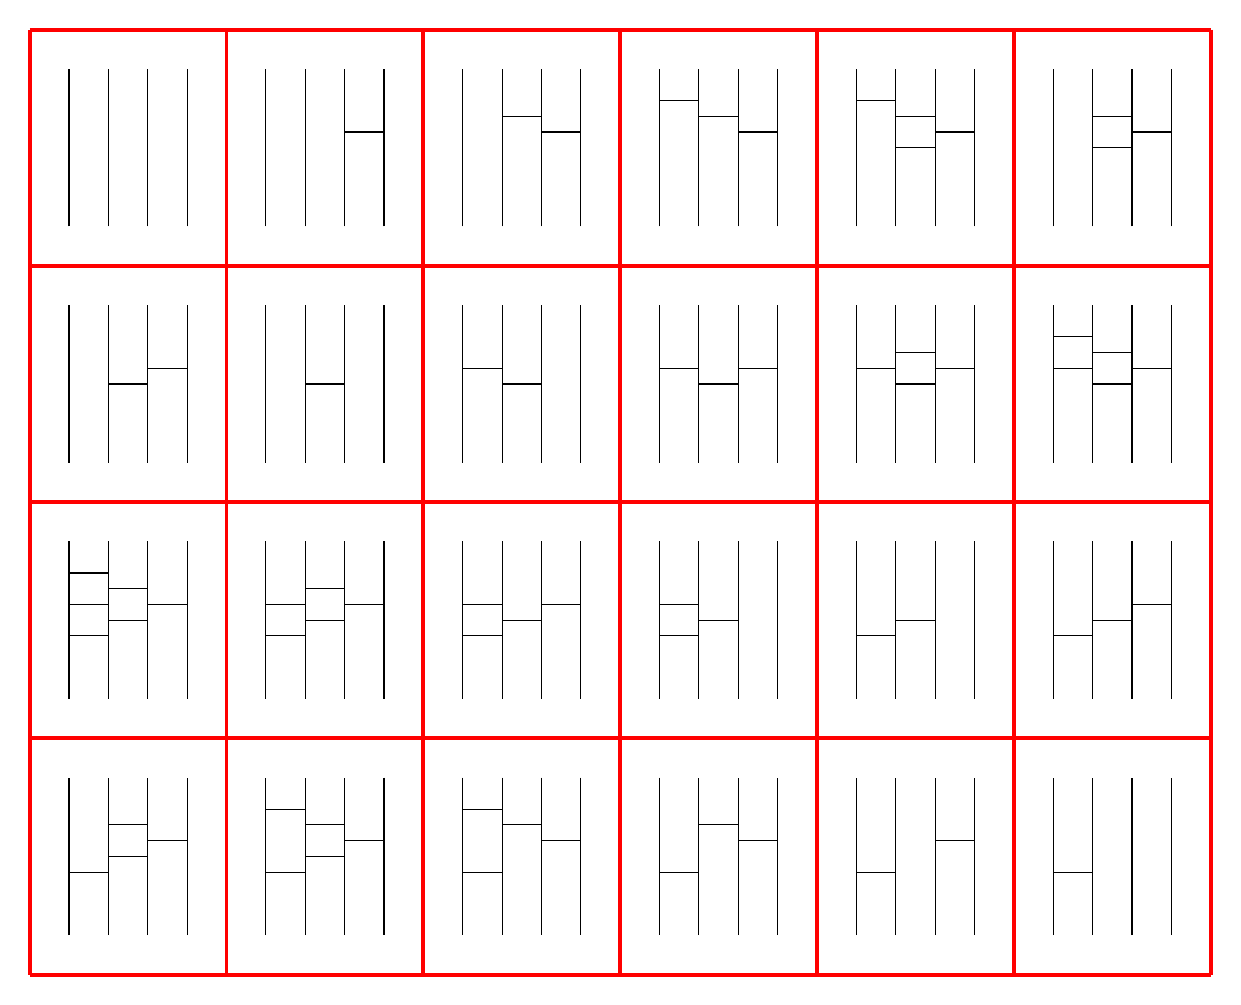
\begin{tikzpicture}
    \draw(0, 0) to (0, 2);
    \draw(0.5, 0) to (0.5, 2);
    \draw(1, 0) to (1, 2);
    \draw(1.5, 0) to (1.5, 2);

    \draw(2.5, 0) to (2.5, 2);
    \draw(3, 0) to (3, 2);
    \draw(3.5, 0) to (3.5, 2);
      \draw(3.5, 1.2) to (4, 1.2);
    \draw(4, 0) to (4, 2);

    \draw(5, 0) to (5, 2);
    \draw(5.5, 0) to (5.5, 2);
      \draw(5.5, 1.4) to (6, 1.4);
    \draw(6, 0) to (6, 2);
      \draw(6, 1.2) to (6.5, 1.2);
    \draw(6.5, 0) to (6.5, 2);

    \draw(7.5, 0) to (7.5, 2);
      \draw(7.5, 1.6) to (8, 1.6);
    \draw(8, 0) to (8, 2);
      \draw(8, 1.4) to (8.5, 1.4);
    \draw(8.5, 0) to (8.5, 2);
      \draw(8.5, 1.2) to (9, 1.2);
    \draw(9, 0) to (9, 2);

    \draw(10, 0) to (10, 2);
      \draw(10, 1.6) to (10.5, 1.6);
    \draw(10.5, 0) to (10.5, 2);
      \draw(10.5, 1.4) to (11, 1.4);
      \draw(10.5, 1) to (11, 1);
    \draw(11, 0) to (11, 2);
      \draw(11, 1.2) to (11.5, 1.2);
    \draw(11.5, 0) to (11.5, 2);

    \draw(12.5, 0) to (12.5, 2);
    \draw(13, 0) to (13, 2);
      \draw(13, 1.4) to (13.5, 1.4);
      \draw(13, 1) to (13.5, 1);
    \draw(13.5, 0) to (13.5, 2);
      \draw(13.5, 1.2) to (14, 1.2);
    \draw(14, 0) to (14, 2);

    %%End of first row
    %%Second row

    \draw(0, -3) to (0, -1);
    \draw(0.5, -3) to (0.5, -1);
      \draw(0.5, -2) to (1, -2);
    \draw(1, -3) to (1, -1);
      \draw(1, -1.8) to (1.5, -1.8);
    \draw(1.5, -3) to (1.5, -1);

    \draw(2.5, -3) to (2.5, -1);
    \draw(3, -3) to (3, -1);
      \draw(3, -2) to (3.5, -2);
    \draw(3.5, -3) to (3.5, -1);
    \draw(4, -3) to (4, -1);

    \draw(5, -3) to (5, -1);
      \draw(5, -1.8) to (5.5, -1.8);
    \draw(5.5, -3) to (5.5, -1);
      \draw(5.5, -2) to (6, -2);
    \draw(6, -3) to (6, -1);
    \draw(6.5, -3) to (6.5, -1);

    \draw(7.5, -3) to (7.5, -1);
      \draw(7.5, -1.8) to (8, -1.8);
    \draw(8, -3) to (8, -1);
      \draw(8, -2) to (8.5, -2);
    \draw(8.5, -3) to (8.5, -1);
      \draw(8.5, -1.8) to (9, -1.8);
    \draw(9, -3) to (9, -1);

    \draw(10, -3) to (10, -1);
      \draw(10, -1.8) to (10.5, -1.8);
    \draw(10.5, -3) to (10.5, -1);
      \draw(10.5, -1.6) to (11, -1.6);
      \draw(10.5, -2) to (11, -2); 
    \draw(11, -3) to (11, -1);
      \draw(11, -1.8) to (11.5, -1.8);
    \draw(11.5, -3) to (11.5, -1);

    \draw(12.5, -3) to (12.5, -1);
      \draw(12.5, -1.4) to (13, -1.4);
      \draw(12.5, -1.8) to (13, -1.8);
    \draw(13, -3) to (13, -1);
      \draw(13, -1.6) to (13.5, -1.6);
      \draw(13, -2) to (13.5, -2);
    \draw(13.5, -3) to (13.5, -1);
      \draw(13.5, -1.8) to (14, -1.8);
    \draw(14, -3) to (14, -1);
    %%End of second row
    \draw(0, -6) to (0, -4);
      \draw(0, -5.2) to (0.5, -5.2);
      \draw(0, -4.4) to (0.5, -4.4);
      \draw(0, -4.8) to (0.5, -4.8);
    \draw(0.5, -6) to (0.5, -4);
      \draw(0.5, -4.6) to (1, -4.6);
      \draw(0.5, -5) to (1, -5);
    \draw(1, -6) to (1, -4);
      \draw(1, -4.8) to (1.5, -4.8);
    \draw(1.5, -6) to (1.5, -4);

    \draw(2.5, -6) to (2.5, -4);
      \draw(2.5, -5.2) to (3, -5.2);
      \draw(2.5, -4.8) to (3, -4.8);
    \draw(3, -6) to (3, -4);
      \draw(3, -4.6) to (3.5, -4.6);
      \draw(3, -5) to (3.5, -5);
    \draw(3.5, -6) to (3.5, -4);
      \draw(3.5, -4.8) to (4, -4.8);
    \draw(4, -6) to (4, -4);

    \draw(5, -6) to (5, -4);
      \draw(5, -5.2) to (5.5, -5.2);
      \draw(5, -4.8) to (5.5, -4.8);
    \draw(5.5, -6) to (5.5, -4);
      \draw(5.5, -5) to (6, -5);
    \draw(6, -6) to (6, -4);
      \draw(6, -4.8) to (6.5, -4.8);
    \draw(6.5, -6) to (6.5, -4);

    \draw(7.5, -6) to (7.5, -4);
      \draw(7.5, -5.2) to (8, -5.2);
      \draw(7.5, -4.8) to (8, -4.8);
    \draw(8, -6) to (8, -4);
       \draw(8, -5) to (8.5, -5);
    \draw(8.5, -6) to (8.5, -4);
    \draw(9, -6) to (9, -4);

    \draw(10, -6) to (10, -4);
          \draw(10, -5.2) to (10.5, -5.2);
    \draw(10.5, -6) to (10.5, -4);
           \draw(10.5, -5) to (11, -5);
    \draw(11, -6) to (11, -4);
    \draw(11.5, -6) to (11.5, -4);

    \draw(12.5, -6) to (12.5, -4);
              \draw(12.5, -5.2) to (13, -5.2);

    \draw(13, -6) to (13, -4);
               \draw(13, -5) to (13.5, -5);

    \draw(13.5, -6) to (13.5, -4);
               \draw(13.5, -4.8) to (14, -4.8);

    \draw(14, -6) to (14, -4);

    %%End of third row

    \draw(0, -9) to (0, -7);
      \draw(0, -8.2) to (0.5, -8.2);
    \draw(0.5, -9) to (0.5, -7);
      \draw(0.5, -8) to (1, -8);
      \draw(0.5, -7.6) to (1, -7.6);
    \draw(1, -9) to (1, -7);
      \draw(1, -7.8) to (1.5, -7.8);
    \draw(1.5, -9) to (1.5, -7);

    \draw(2.5, -9) to (2.5, -7);
      \draw(2.5, -7.4) to (3, -7.4);
      \draw(2.5, -8.2) to (3, -8.2);
    \draw(3, -9) to (3, -7);
      \draw(3, -8) to (3.5, -8);
      \draw(3, -7.6) to (3.5, -7.6);
    \draw(3.5, -9) to (3.5, -7);
       \draw(3.5, -7.8) to (4, -7.8);
    \draw(4, -7) to (4, -9);

    \draw(5, -7) to (5, -9);
      \draw(5, -7.4) to (5.5, -7.4);
      \draw(5, -8.2) to (5.5, -8.2);
    \draw(5.5, -7) to (5.5, -9);
      \draw(5.5, -7.6) to (6, -7.6);
    \draw(6, -7) to (6, -9);
           \draw(6, -7.8) to (6.5, -7.8);
    \draw(6.5, -7) to (6.5, -9);

    \draw(7.5, -7) to (7.5, -9);
          \draw(7.5, -8.2) to (8, -8.2);
    \draw(8, -9) to (8, -7);
        \draw(8, -7.6) to (8.5, -7.6);
    \draw(8.5, -9) to (8.5, -7);
               \draw(8.5, -7.8) to (9, -7.8);
    \draw(9, -9) to (9, -7);

    \draw(10, -9) to (10, -7);
      \draw(10, -8.2) to (10.5, -8.2);
    \draw(10.5, -9) to (10.5, -7);
    \draw(11, -9) to (11, -7);
      \draw(11, -7.8) to (11.5, -7.8);
    \draw(11.5, -9) to (11.5, -7);

    \draw(12.5, -9) to (12.5, -7);
              \draw(12.5, -8.2) to (13, -8.2);
    \draw(13, -9) to (13, -7);
    \draw(13.5, -9) to (13.5, -7);
    \draw(14, -9) to (14, -7);

    %%end fourth row

    %%draw the border

    \draw [line width=0.5mm, red ] (-0.5,2.5) to (-0.5,-9.5);
    \draw [line width=0.5mm, red ] (2,2.5) to (2,-9.5);
    \draw [line width=0.5mm, red ] (4.5,2.5) to (4.5,-9.5);
    \draw [line width=0.5mm, red ] (7,2.5) to (7,-9.5);
    \draw [line width=0.5mm, red ] (9.5,2.5) to (9.5,-9.5);
    \draw [line width=0.5mm, red ] (12,2.5) to (12,-9.5);
    \draw [line width=0.5mm, red ] (14.5,2.5) to (14.5,-9.5);

   \draw [line width=0.5mm, red ] (-0.5,2.5) to (14.5,2.5);
   \draw [line width=0.5mm, red ] (-0.5,-0.5) to (14.5,-0.5);
      \draw [line width=0.5mm, red ] (-0.5,-3.5) to (14.5,-3.5);
   \draw [line width=0.5mm, red ] (-0.5,-6.5) to (14.5,-6.5);
   \draw [line width=0.5mm, red ] (-0.5,-9.5) to (14.5,-9.5);





  \end{tikzpicture}
  \end{center}
  \caption{The table of $CanL{\pi_{4}}$ generated using the modified SJT algorithm. The table is to be read from top left to bottom right. Note that each ladder is the root ladder from each corresponding $OptL{\pi_{4}}$}
\end{figure}

%%end proof


From the above figure, it should be clear that the canonical representative from $CanL{\pi_{N}}$ when using the 
modified SJT algorithm is the root ladder from each $OptL{\pi_{N}}$. Recall that the root ladder is the 
ladder whose bars of a lesser route have not crossed the bars of a greater route. In the case of the 
modified sjt algorithm, transitioning from $L_{i}$ to $L_{i+1}$ involves simply inserting a new bar 
or removing a bar for a given route. Let $K$ be the current route. If a new bar being added belongs to 
route $K$, then the addition of the bar does not violate the property of the root ladder. If the new bar to
be added belongs to route $K-1$, then the bar is added below $K's$ bars, still not violating the property of 
the root ladder. When a bar is removed, that implies it has already been added. Let $L_{i}$ be a 
ladder whose bar is about to be removed, thus transitioning to $L_{i+1}$. Let $L_{i}$ be a root ladder
, then removing a bar from $L_{i}$ cannot make $L_{i+1}$ a non-root ladder, because 
removing a bar from $L_{i}$ does not allow the bar of a lesser element to cross the bars of a greater element.
Thus, the canonical representative for $CanL{\pi_{N}}$ is always the root ladder from each $OptL{\pi_{N}}$.\par 



%%Beging the cases
The calculations for the row and column for the bar 
depend on several factors. The first factor is whether the row and column is being calculated for $K=N$ or 
if $K < N$. If $K=N$, then the row and column are calculated using the main function, modifiedSJT. The second factor 
is whether a bar is being removed from the ladder or a bar is being added to the ladder. Therefore, there are eight cases 
to consider. The cases are the following: 
\begin{caseof}
  \case{$Route = N$}{Bar is being added. Row is being calculated.}
  \case{$Route = N$}{Bar is being added. Column is being calculated.}
  \case{$Route = N$}{Bar is being removed. Row is being calculated.}
  \case{$Route = N$}{Bar is being removed. Column is being calculated.}
  \case{$Route < N$}{Bar is being added. Row is being calculated.}
  \case{$Route < N$}{Bar is being added. Column is being calculated.}
  \case{$Route < N$}{Bar is being removed. Row is being calculated.}
  \case{$Route < N$}{Bar is being removed. Column is being calculated.}
\end{caseof}

%%End the cases

When proving the above cases, keep in mind that the ladder, $L$, is a two dimensional array with $2(N-1)-1$ rows and $(N-1)$ columns.

%%proof 1
\begin{lemma}
  Let $route=N$. Let $I=$ the current number of bars in the ladder belonging to route $N$. 
  Assume a bar is being added. Then the $row=(N-1)-I$.
\end{lemma}
\begin{proof}
  Keeping in mind we are only dealing with root ladders, then the bars of the $Nth$ route will be above the bars of 
  any other route. The bars are added bottom right to top left, and no two bars of the $Nth$ route can be on the same row, 
  for having two bars of the same route on the same row violates the constraint that no two endpoints of two bars can be toucing.
  There are a total of $N-1$ rows requried for the bars of the $Nth$ route. $I$ is incremented for each bar that is added 
  to the $Nth$ route. The first bar to be added will be at row $N-1$, once it is added $I$ is incremented by one, the second 
  bar of the $Nth$ route will be added to row $N-2$, which equals $N-1-I$. Then $I$ is incremented again. This continues 
  until all bars of the $Nth$ route are added. Refer to figure --fig for an example of row calulation when adding a bar 
  for the $Nth$ route.
\end{proof}\pagebreak


\begin{figure}[!htp]
  \begin{center}
    \begin{tikzpicture}
      \draw(0, 0) to (0, 6);
      \draw(2, 0) to (2, 6);
        \node at(3, 4.7){4,2};
        \draw(2, 4.5) to (4, 4.5);
      \draw(4, 0) to (4, 6);
        \node at(5, 3.7){4,3};
        \draw(4, 3.5) to (6, 3.5);
      \draw(6, 0) to (6, 6);

      \node at(-2, 5.5){R1};
      \node at(-2, 4.5){R2};
      \node at(-2, 3.5){R3};
      \node at(-2, 2.5){R4};
      \node at(-2, 1.5){R5};

      \node at(0, 6.2){1};
      \node at(2, 6.2){4};
      \node at(4, 6.2){2};
      \node at(6, 6.2){3};

      \draw (1,5.5) ellipse (1cm and .4cm);

    \end{tikzpicture}
  \end{center}
  \caption{The row of the last bar to be added for element $4$ is row $1$. $row=1=3-2=(N-1)-I$}
\end{figure}

%%end proof 1


%%Prove case 2
\begin{lemma}
  Let $route=N$. Let $I=$ the current number of bars in the ladder belonging to route $N$. 
  Assume a bar is being added. Then the $column=(N-1)-I$.
\end{lemma}
\begin{proof}
  Keeping in mind we are only dealing with root ladders, then the bars of the $Nth$ route will be above the bars of 
  any other route. The bars are added bottom right to top left. The ladder has a total of $N-1$ columns, seeing as 
  the $Nth$ element has $N-1$ bars, each requiring their own column. If two bars of the $Nth$ element were 
  in the same column, then this would violate one of two constraints. Either the two bars would be directly 
  above/below each other, in which case the ladder would not be optimal seeing as the two elements that crossed the 
  top bar would then cross the bottom bar, which means the ladder has an extra bar. The second case can be discredited as 
  follows. Let the top bar belonging to route $N$ be designated as $X$, let the bottom bar belonging to route $N$ be 
  designated as $Y$. Assume $X$ and $Y$ are in the same column.
  Then there is some third bar $Z$, not belonging to route $N$ and not in the same column 
  as $X$ and $Y$ such that $Z$ is in the column directly to the left or right of the column of $X$ and $Y$. But if that 
  is the case, then $Z$ is above bar $Y$ which violates the definition of the root ladder. Therefore, every bar 
  belonging to route $N$ requires its own column. The first bar to be added to route $N$ goes in the rightmost column which 
  equals column $N-1$, then $I$ is incremented by one. The second bar is in columb $(N-1)-1=(N-1)-I$ and $I$ is incremented 
  by one. The process continues until all $(N-1)$ bars of the $Nth$ route have been added. See figure --fig for an example 
  of column calculation.
\end{proof}

\begin{figure}[!htp]
  \begin{center}
    \begin{tikzpicture}
       \draw(0, 0) to (0, 6);
      \draw(2, 0) to (2, 6);
        \node at(3, 4.7){4,2};
        \draw(2, 4.5) to (4, 4.5);
      \draw(4, 0) to (4, 6);
        \node at(5, 3.7){4,3};
        \draw(4, 3.5) to (6, 3.5);
      \draw(6, 0) to (6, 6);

      \node at(1, -0.3){Col 1};
      \node at(3, -0.3){Col 2};
      \node at(5, -0.3){Col 3};

      \node at(0, 6.2){1};
      \node at(2, 6.2){4};
      \node at(4, 6.2){2};
      \node at(6, 6.2){3};

      \draw (1,5.5) ellipse (1cm and .4cm);


      
    \end{tikzpicture}
  \end{center}
  \caption{The column of the last bar to be added for element $4$ is $1$. $column=1=3-2=(N-1)-I$}
\end{figure}
%%End proof of case 2


%%Proof of case 3
\begin{lemma}
  Let $route=N$. Let $I=$ the current number of bars that have been removed from route $N$. Assume a bar is being removed. 
  Then the $row=I+1$
\end{lemma}
\begin{proof}
  Keeping in mind we are dealing with root ladders and bars are removed from left to right, top to bottom, then the first bar to 
  be removed from route $N$ is at row one. Since no bars have been removed, $I$ currently equals zero, 
  thus row $1=I+1$. Once removed, $I$ is increased by one, indicating a bar has been removed. The next bar is at row two, 
  which again equals $I+1$. Continue until all bars of the $Nth$ route have been removed. See figure --fig for an example 
  of row calculation when removing a bar for the $Nth$ element.
\end{proof}
\begin{figure}[!htp]
  \begin{center}
    \begin{tikzpicture}
      \draw(0, 0) to (0, 6);
        \draw [dashed] (0,5.5) -- (2,5.5);
      \draw(2, 0) to (2, 6);
        \node at(3, 4.7){4,2};
        \draw(2, 4.5) to (4, 4.5);
      \draw(4, 0) to (4, 6);
        \node at(5, 3.7){4,3};
        \draw(4, 3.5) to (6, 3.5);
      \draw(6, 0) to (6, 6);

      \node at(-2, 5.5){R1};
      \node at(-2, 4.5){R2};
      \node at(-2, 3.5){R3};
      \node at(-2, 2.5){R4};
      \node at(-2, 1.5){R5};

      \node at(0, 6.2){1};
      \node at(2, 6.2){4};
      \node at(4, 6.2){2};
      \node at(6, 6.2){3};

      \draw (3,4.5) ellipse (1cm and .4cm);

    \end{tikzpicture}
  \end{center}
  \caption{The row of the second bar to be removed from element $4's$ route is row $2$. The dashed bar indicates that it has already been 
  removed from $4's$ route. $I$ is the number of bars currently removed from $4's$ route, which is currently $1$. Therefore $row=2=I+1$}
\end{figure}

%%End of proof of case 3


%%Proof Case 4
\begin{lemma}
  Let $route=N$. Let $I=$ the current number of bars that have been removed from route $N$. Assume a bar is being removed.
  Then the $column=I+1$.
\end{lemma}
\begin{proof}
  Keeping in mind we are dealing with root ladders and bars are removed from left to right, top to bottom, then the first bar to 
  be removed from route $N$ is at column one. Since no bars have been removed, $I$ currently equals zero, 
  thus column $1=I+1$. Once removed, $I$ is increased by one, indicating a bar has been removed. The next bar is at column two, 
  which again equals $I+1$. Continue until all bars of the $Nth$ route have been removed. See figure --fig for an example 
  of column calculation when removing a bar from the $Nth$ route.
\end{proof}

\begin{figure}[!htp]
  \begin{center}
    \begin{tikzpicture}
      \draw(0, 0) to (0, 6);
        \draw [dashed] (0,5.5) -- (2,5.5);

      \draw(2, 0) to (2, 6);
        \node at(3, 4.7){4,2};
        \draw(2, 4.5) to (4, 4.5);
      \draw(4, 0) to (4, 6);
        \node at(5, 3.7){4,3};
        \draw(4, 3.5) to (6, 3.5);
      \draw(6, 0) to (6, 6);

      \node at(1, -0.3){Col 1};
      \node at(3, -0.3){Col 2};
      \node at(5, -0.3){Col 3};

      \node at(0, 6.2){1};
      \node at(2, 6.2){4};
      \node at(4, 6.2){2};
      \node at(6, 6.2){3};

      \draw (3,4.5) ellipse (1cm and .4cm);


      
    \end{tikzpicture}
  \end{center}
  \caption{The column of the second bar to be removed from element $4's$ route is row $2$. The dashed bar indicates that it has already been 
  removed from $4's$ route. $I$ is the number of bars currently removed from $4's$ route, which currently is $1$. Therefore $column=2=I+1$}
\end{figure}
%%End of proof of case 4



%%Proof of case 5
\begin{lemma}
  Let $arr$ be a one indexed array. Let $2 \leq K < N$ be the $Kth$ element to have a bar added to its route. 
  Let $arr[K]$ represent the number of bars for route $K$ that are currently in the 
  ladder. Let $L_{i}$ be a two dimensional, one indexed array representing the current ladder.
  The the row for the current bar to be added for route $K$ is $Row=(N-1) + (N-K) - arr[K]$.
\end{lemma}
\begin{proof}
   It must be noted that we are listing only root ladders. So when transitioning from 
$L_{i}$ to $L_{i+1}$ in $CanL{\pi_{N}}$ both are root ladders. Recall that the root ladder is the ladder such that no  
route of any lesser value in $\pi$ has crossed the route of a greater value. With this in mind, one can say that the 
number of rows required for the $Nth$ value is $N-1$ seeing as the $Nth$ value can have at most $N-1$ bars in its route, each requiring  their own 
row. Since bars are added right to left, bottom, up, then the first bar of route $K$ will be added to the row 
just  below the last bar of the previous route. The reason $N-1$ is added is because the $Nth$ element requires 
$N-1$ rows in $L$. If $K$ is one less than $N$ then 
the first bar of $K$ will be added one row below the last bar of $N$. If $K$ is two less than $N$ then the first bar 
of $K$ will be added two rows below the last bar of $N$, etc. The $(N-K)$ is added because 
the difference between $N$ and $K$ is the offset of the difference in rows between the lowest/first bar of $N$ 
and the lowest/first bar of $K$. When a bar is added to $K's$ route, the $arr[k]$ is incremented by one. This value is subtracted in 
order to effectively move up the ladder as bars are added to $K's$ route from bottom right to top left. See figure for an example of 
row calculation when adding a bar for $K < N$.
\end{proof}\pagebreak

\begin{figure}[!htp]
  \begin{center}
    
    \begin{tikzpicture}

    \draw(0, -2) to (0, 6);
       \draw(0, 5.5) to (2, 5.5);
       \node at (1, 5.7){5,1};
       \node at (-1, 5.5){R1};
     \draw(2, -2) to (2, 6);
       \draw(2, 4.5) to (4, 4.5);
       \draw(2, 0.5) to (4, 0.5);
       \node at (3, 4.7){5,3};
       \node at(3, 0.7){3, 2};
       \node at(-1, 4.5){R2};
     \draw(4, -2) to (4, 6);
       \draw(4, 3.5) to (6, 3.5);
       \node at(5, 3.7){5,2};
       \node at(-1, 3.5){R3};
     \draw(6, -2) to (6, 6);
       \draw(6, 2.5) to (8, 2.5);
       \node at(7, 2.7){5,4};
       \node at(-1, 2.5){R4};
     \draw(8, -2) to (8, 6);

    \node at(-1, 1.5){R5};
    \node at(-1, 0.5){R6};
    \node at(-1, -0.5){R7};
    \draw (1,1.5) ellipse (1cm and .4cm);

  \end{tikzpicture}

\end{center}
\caption{The second bar of route 3 goes will go in row 5, column 1. $5 = (5-1)+(5-3)-1 = (N-1)+(N-K)-arr[K]$.}
\end{figure}
%%End of prof of case 5


%%Proof of case 6
\begin{lemma}
  Let $arr$ be a one indexed array. Let $2 \leq K < N$ be the $Kth$ element to have a bar added to its route. 
  Let $arr[K]$ represent the number of bars for route $K$ that are currently in $L$. 
  The the column for the current bar to be added for route $K$ is $Column=(K-1)-arr[K]$.
\end{lemma}
\begin{proof}
  The total number of bars required for route $K$ is $K-1$, each requring their own column. The reason each 
  bar requires its own column is the same for when the route equals $N$. See the proof for lemma 3.1.5. The 
  bars are added right to left and when a bar is added $arr[K]$ is incremented by one. The initial column to add the first bar 
  of route $K$ is column $K-1$. This is because the first bar of the $Kth$ route is the left child bar of the 
  lowest bar of the $K+1th$ route. Denote the first bar to be added of the $Kth$ route as $Y$ and the 
  lowest bar of the $K+1th$ route as $X$. $X$ is the parent bar of $Y$ and $Y$ is the left child bar of 
  $X$ for the following reasosn. If $Y$ was directly below $X$, then the ladder would have redundant bars, thus making it 
  non-optimal. If $Y$ was to the right of $X$, then $Y$ would either be above $X$, thus violating the property of the root ladder, 
  or if $Y$ were below $X$ and to the right of $X$ then $Y$ would be part of the route for $K+1$, yet this is a contradiction 
  seeing as we said $Y$ belongs to $K's$ route. Therefore, $Y$ must be in a column to the left of $X$. As bars are added 
  to $K's$ route, $arr[K]$ is incremented for each bar. It is subtracted from the original column, $K-1$, effectively moving 
  to the next column to the left in $L$. See figure --fig for an example of column calculation when adding a bar for $K<N$.
\end{proof}
\begin{figure}[!htp]
  \begin{center}
    
    \begin{tikzpicture}

    \draw(0, -2) to (0, 6);
       \draw(0, 5.5) to (2, 5.5);
       \node at (1, 5.7){5,1};
     \draw(2, -2) to (2, 6);
       \draw(2, 4.5) to (4, 4.5);
       \draw(2, 0.5) to (4, 0.5);
       \node at (3, 4.7){5,3};
       \node at(3, 0.7){3, 2};
     \draw(4, -2) to (4, 6);
       \draw(4, 3.5) to (6, 3.5);
       \node at(5, 3.7){5,2};
     \draw(6, -2) to (6, 6);
       \draw(6, 2.5) to (8, 2.5);
       \node at(7, 2.7){5,4};
     \draw(8, -2) to (8, 6);

    \draw (1,1.5) ellipse (1cm and .4cm);

    \node at(1, -2.3){Col 1};
    \node at(3, -2.3){Col 2};
    \node at(5, -2.3){Col 3};
    \node at(7, -2.3){Col 4};
  \end{tikzpicture}
\end{center} 
\caption{The second bar of route $K=3$ goes will go in column 1. Since one bar has been added, $arr[3]=1$. $col=1=2-1=(K-1)-arr[K]$.}
\end{figure}

%%End of proof of case 6


%%Proof of case 7
\begin{lemma}
  Let $arr$ be a one indexed array. Let $2 \leq K < N$ be the $Kth$ element to have a bar removed from its route. 
  Let $arr[K]$ represent the number of bars for route $K$ that have currently been removed from the ladder. 
  The the row for the current bar to be removed for route $K$ is $Row=(N-1) + (N-K) + arr[K] - (K-2)$.
\end{lemma}
\begin{proof}
  When removing a bar the row is calculated as follows. Keeping in mind bars are removed from top to bottom, left to right.
  The $Nth$ element requries the first $(N-1)$ rows. Which is why $(N-1)$ is added. The last bar to be removed of the $Kth$ route is $(N-K)$
  rows below row $(N-1)$ which is why $(N-K)$ is added. $arr[K]$ is added to effectively move down the ladder 
  for each remaining bar of the $Kth$ route in the ladder left to be removed. Since the first bar of the $Kth$ route 
  to be removed is highest up the ladder, every subsequent bar to be removed from the $Kth$ route requires 
  moving down the ladder from the row of first bar of the $Kth$ route; this is accomplished by adding $array[K]$ which 
  indicates how many bars are currently removed from the $Kth$ route. Lastly, $(K-2)$  is subtracted in order to 
  get to the row of the first bar of the $Kth$ route. The difference between the row of the last bar of the $Kth$ route and 
  the first bar of the $Kth$ route is $K-2$. Seeing as the $Kth$ route has at most $K-1$ bars, each requiring their own row, then the 
  first bar of the $Kth$ route is $K-2$ rows higher than the last bar of the $Kth$ route. See figure fig for 
  an example of removing a bar.\pagebreak
\end{proof}

\begin{figure}[!htp]
  \begin{center}
    \begin{tikzpicture}
      \draw(0, 0) to (0, 8);
        \draw(0, 7) to (2, 7);
          \node at (1, 7.3){5,4};
          \draw [dashed] (0,5) -- (2,5);

        \draw(0, 1) to (2, 1);
          \node at (1, 1.3){2, 1};
        
      
      \draw(2, 0) to (2, 8);
        \draw(2, 6) to (4, 6);
          \node at (3, 6.3){5, 2};
        \draw(2, 4) to (4, 4);
          \node at (3, 4.3){4, 1};
      \draw(4, 0) to (4, 8);
        \node at(5, 5.3){5, 1};
        \draw(4, 5) to (6, 5);
          \node at(5, 3.3){4, 3};
        \draw(4, 3) to (6, 3);
      
      \draw(6, 0) to (6, 8);
        \draw(6, 4) to (8, 4);
        \node at (7, 4.3){5, 3};
      \draw(8, 0) to (8, 8);

      \node at (-2, 7){R1};

      \node at (-2, 6){R2};

      \node at (-2, 5){R3};
      \node at(-2, 4){R4};
      \node at (-2, 3){R5};
      \node at (-2, 2){R6};
      \node at(-2, 1){R7};
      \draw (3,4) ellipse (1cm and .4cm);

    \end{tikzpicture}
  \end{center}
  \caption{The bar to be removed for route $K=4$ is (4, 1) which is at row 4. The dashed line indicates a bar 
  from route $4$ has already been removed. $row= 4 = (5-1)+(5-4)+ 1 - (2) = (N-1)+(N-K) + arr[K] - (K-2)$.}
\end{figure}
%%End of proof of case 7

%%Proof of case 8
\begin{lemma}
   Let $arr$ be a one indexed array. Let $2 \leq K < N$ be the $Kth$ element to have a bar removed from its route. 
  Let $arr[K]$ represent the number of bars for route $K$ that have currently been removed from the ladder. 
  Then the column for the current bar to be removed for route $K$ is $Column=arr[K]+1$.
\end{lemma}
\begin{proof}
  The bars are removed left to right. The first bar to be removed is the leftmost bar belonging to route $K$ which 
  is always at column $1$. This is because the number of columns required for the $K-1$ bars is $K-1$, terminating at 
  column number $K-1$. Thus, the first bar to be removed must always be at column $1$ and the last bar to 
  be removed is at column $K-1$. $arr[K]$ is incremented for each bar removed from the route of $K$.
\end{proof}

\begin{figure}[!htp]
  \begin{center}
    \begin{tikzpicture}
      \draw(0, 0) to (0, 8);
        \draw(0, 7) to (2, 7);
          \node at (1, 7.3){5,4};
          \draw [dashed] (0,5) -- (2,5);

        \draw(0, 1) to (2, 1);
          \node at (1, 1.3){2, 1};
        
      
      \draw(2, 0) to (2, 8);
        \draw(2, 6) to (4, 6);
          \node at (3, 6.3){5, 2};
        \draw(2, 4) to (4, 4);
          \node at (3, 4.3){4, 1};
      \draw(4, 0) to (4, 8);
        \node at(5, 5.3){5, 1};
        \draw(4, 5) to (6, 5);
          \node at(5, 3.3){4, 3};
        \draw(4, 3) to (6, 3);
      
      \draw(6, 0) to (6, 8);
        \draw(6, 4) to (8, 4);
        \node at (7, 4.3){5, 3};
      \draw(8, 0) to (8, 8);


      \node at (1, -0.3){Col 1};
      \node at(3, -0.3){Col 2};
      \node at (5, -0.3){Col 3};
      \node at (7, -0.3){Col 4};
      \draw (3,4) ellipse (1cm and .4cm);

    \end{tikzpicture}
  \end{center}
  \caption{The bar to be removed for route $K=4$ is (4, 1) which is at column 2. The dashed line indicates a bar 
  from route $4$ has already been removed. Since one bar from routr $4$ has been removed, $arr[4]=1$. $column= 2 = 1+1 = arr[K] + 1$.}
\end{figure}
%%End of proof of case 8
\subsection{Cyclic Inversion}
\begin{algorithm}
  \caption{First part of the algorithm Cyclic Inversion}
  \begin{algorithmic}[1]
    \Function{CyclicInversion}{$Ladder[2(N-1)-1][N-1]$, $CurrentLimit$, $MaxLimit$, $N$, $K$}


      
      %%base case
      \If{the number of bars in $Ladder=CurrentLimit$}
        \State $print(Ladder)$
        \State return
      \EndIf

      %%
      \If{$CurrentLimit > MaxLimit$}
        \State return
      \EndIf

      %%If K=N
     \If{$K=N$}

      \State {$M \gets 0$}
      \State $Row \gets K-1$
      \State $Col \gets K-1$
      \State $NumBars \gets$ current number of bars in $Ladder$
      %%While
      \While{$NumBars < CurrentLimit$ AND $M < K-1$}
        \State $Ladder[Row][Col] \gets 1$
        \State $Row \gets row-1$
        \State $Col \gets col-1$
        \State $M \gets M+1$
        \State $NumBars \gets NumBars+1$
      \EndWhile
      %%End while

      \If{$NumBars = CurrentLimir$}
        \State $PrintLadder(Ladder)$
      \EndIf
      \State remove upper leftmost bar belonging to $K's$ route.
      \State return

    \algstore{aaa}

  \end{algorithmic}
\end{algorithm}

\begin{algorithm}
  \caption{Cyclic Inversion Continued}
    \begin{algorithmic}[1]
          \algrestore{aaa}

    \Else 
      \State $count \gets 0$
      \For{$I \gets 0$, $I < K$, $I \gets I+1$}
       \If{the number of bars in $Ladder=CurrentLimit$}
            \State break
        \EndIf

        \If{$I = 0$}
          \State CyclicInversion(Ladder, CurrentLimit, MaxLimit, N, $K+1$)
      
       
        
        \Else
          \State $Row \gets (N-1) + (N-K) - count$
          \State $Column \gets (K-1)-arr[K]$
          \State $Ladder[Row][Col] \gets 1$
          \State $count \gets count + 1$
          \State CyclicInversion(Ladder, CurrentLimit, MaxLimit, N, $K+1$)
        \EndIf
      \EndFor
      \State remove all bars from $K's$ route.

    \EndIf
    \EndFunction
  \end{algorithmic}
\end{algorithm}


\begin{algorithm}
  \caption{Driver for the Cyclic Inversion Algorithm}
  \begin{algorithmic}[1]
    \Function{Cylclic Inversion Driver}{$Ladder[2(N-1)-1][N-1]$, $N$}
      \State $MaxLimit \gets (N(N-1))/2$
      \State $K \gets 2$
      \For{$I \gets 0, I <= MaxLimit, I \gets I+1$}
        \State CyclicInversion($Ladder$, $CurrentLimit \gets I$, $MaxLimit$, $N$, $K$)

      \EndFor

    \EndFunction
  \end{algorithmic}
\end{algorithm}\pagebreak

The initial conditions for the algorithm are the following. Let $Ladder$ be initialized as a two dimensional array with $2(N-1)-1$ rows and $(N-1)$ columns.  Let $N$ be initialized to the maximal element in $\pi_{N}$. Let $K$ be initialized to $2$.
Let the $MaxLimit$ be initialized to $(N(N-1))/2$.Let the $CurrentLimit$ be initialized to zero. The way the algorithm works is the following. The $CurrentLimit$ 
represents the number of bars to be inserted into $Ladder$. Once all ladders with $CurrentLimit$ bars have been created, the $CurrentLimit$ is increased by one 
and the algorithm repeats until $CurrenLimit > MaxLimit$. This creates all ladders in $CanL{\pi_{N}}$. The ladders are generated as a forest structure,
 with each value of $CurrentLimit$ creating its own tree of ladders. See figure --fig for the 
forest of ladders for $N=4$. The forest of ladders is all the ladders in $CanL{\pi_{N}}$. On each recursive call to the function, $K$ is increased by one until $K=N$. When $K=N$ all the remaining bars that need to 
be added to the ladder are added to $K=N's$ route. Then the bars of $K=N's$ route are removed and relocated to the bars of $K-1's$ route. This process 
repeats itself until all the combinations of bars for the $CurrentLimit$ are inserted. Each combination of bars into the $Ladder$ 
data structure creates a unique ladder from each $OptL{\pi_{N}}$, thus adding one more ladder to $CanL{\pi_{N}}$.
Once complete, the tree of ladders terminates, and the $CurrentLimit$ increases, thus creating a new tree in the forest for 
$CanL{\pi_{N}}$.\pagebreak

\begin{figure}[!htp]
  %%first tree
 
      
     
    \begin{minipage}{.8\textwidth}
     
         \begin{tikzpicture}
          \node at (-1, 1){\tiny $bars=0$};
          \draw(0, 0) to (0, 1);
          \draw(0.2, 0) to (.2, 1);
          \draw(.4, 0) to (.4, 1);
          \draw(.6, 0) to (.6, 1);
        \end{tikzpicture}\hspace{20mm}
     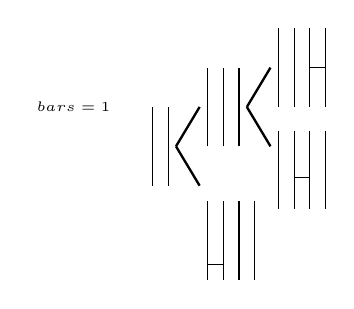
\begin{tikzpicture}
        \node at (-1, 1){\tiny $bars=1$};
        %%l1
          \draw(0, 0) to (0, 1);
          \draw(.2, 0) to (.2, 1);
                      \draw[line width=0.3mm] (.3, .5) to (.6, 1);
                      \draw[line width = .3mm](.3, .5) to (.6, 0);
          %%l2
          \draw(.7, .5) to (.7, 1.5);
          \draw(.9, .5) to (.9, 1.5);
          \draw(1.1, 0.5) to (1.1, 1.5);


            \draw[line width = .3mm](1.2, 1) to (1.5, 1.5);
            \draw[line width = .3mm](1.2, 1) to (1.5, 0.5);
          %%t3 terminate
          \draw(1.6, 1) to (1.6, 2);
          \draw(1.8, 1) to (1.8, 2);
          \draw(2, 1) to (2, 2);
            \draw(2, 1.5) to (2.2, 1.5);
          \draw(2.2, 1) to (2.2, 2);

          %l4 terminate
          \draw(.7, -0.2) to (.7, -1.2);
            \draw(.7, -1) to (.9,-1);
          \draw(.9, -.2) to (.9, -1.2);
          \draw(1.1, -.2) to (1.1, -1.2);
          \draw(1.3, -0.2) to (1.3, -1.2);

          %l5 terminate
          \draw(1.6, .7) to (1.6, -.3);
          \draw(1.8, .7) to (1.8, -.3);
            \draw(1.8, .1) to (2, .1);
          \draw(2, .7) to (2, -.3);
          \draw(2.2, .7) to (2.2, -.3);
        
      \end{tikzpicture}
      

               
    \end{minipage}\\~\\

   %%t3
  \begin{minipage}{.8\textwidth}
     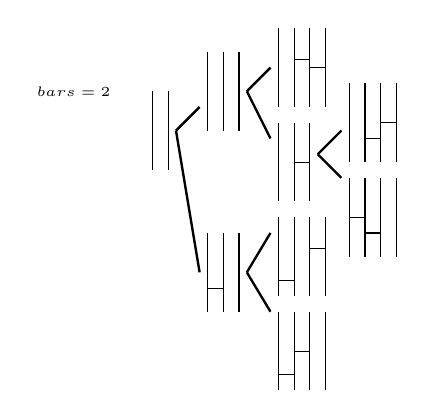
\begin{tikzpicture}
       \node at (-1, 1){\tiny $bars=2$};

        %%L1
        \draw(0, 0) to (0, 1);
        \draw(.2, 0) to (.2, 1);
        
          \draw[line width=.3mm] (.3, .5) to (.6, .8);
          \draw[line width = .3mm](.3, .5) to (.6, -1.3);

        
        \draw(.7, -.8) to (.7, -1.8);
          \draw(.7, -1.5) to (.9, -1.5);
        \draw(.9, -.8) to (.9, -1.8);
        \draw(1.1, -.8) to (1.1, -1.8);

          \draw[line width = .3mm](1.2, -1.3) to (1.5, -.8);
          \draw[line width = .3mm](1.2, -1.3) to (1.5, -1.8);
        
        %%terminate
        \draw(1.6, -.6) to (1.6, -1.6); 
          \draw(1.6, -1.4) to (1.8, -1.4);
         \draw(1.8, -.6) to (1.8, -1.6);  
         \draw(2, -.6) to (2, -1.6);  
            \draw(2, -1) to (2.2, -1); 
         \draw(2.2, -.6) to (2.2, -1.6);
         
         %%terminate
         \draw(1.6, -1.8) to (1.6, -2.8);
          \draw(1.6, -2.6) to (1.8, -2.6);
         \draw(1.8, -1.8) to (1.8, -2.8);
          \draw(1.8, -2.3) to (2, -2.3);
         \draw(2, -1.8) to (2, -2.8);
         \draw(2.2, -1.8) to (2.2, -2.8);



        %%L2 
        \draw(.7, .5) to (.7, 1.5);
        \draw(.9, .5) to (.9, 1.5);
        \draw(1.1, .5) to (1.1, 1.5);

          \draw[line width = .3mm](1.2, 1) to (1.5, 1.3);
          \draw[line width = .3mm](1.2, 1) to (1.5, .4);
        
        %%L3 terminate
        \draw(1.6, .8) to (1.6, 1.8);
        \draw(1.8, .8) to (1.8, 1.8);
          \draw(1.8, 1.4) to (2, 1.4);
        \draw(2, .8) to (2, 1.8);
          \draw(2, 1.3) to (2.2, 1.3);
        \draw(2.2, .8) to (2.2, 1.8);

        %L4 
        \draw(1.6, .6) to (1.6, -.4);
        \draw(1.8, .6) to (1.8, -.4);
          \draw(1.8, .1) to (2, .1);
        \draw(2, .6) to (2, -.4);
          \draw[line width = .3mm](2.1, .2) to (2.4, .5);
          \draw[line width = .3mm](2.1, .2) to (2.4, -.1);
        
        %L5 terminate
        \draw(2.5, .1) to (2.5, 1.1);
        \draw(2.7, .1) to (2.7, 1.1);
          \draw(2.7, .4) to (2.9, .4);
        \draw(2.9, .1) to (2.9, 1.1);
          \draw(2.9, .6) to (3.1, .6);
        \draw(3.1,.1) to (3.1, 1.1);

        %L6 terminate
        \draw(2.5, -.1) to (2.5, -1.1);
          \draw(2.5, -.6) to (2.7, -.6);
        \draw(2.7, -.1) to (2.7, -1.1);
          \draw(2.7, -.8) to (2.9, -.8);
        \draw(2.9, -.1) to (2.9, -1.1);
        \draw(3.1, -.1) to (3.1, -1.1);


      \end{tikzpicture}\hspace{10mm}
      \begin{tikzpicture}
      \node at (-1, 1){\tiny $bars=3$};

        %%L1
           \draw(0, 0) to (0, 1);
           \draw(.2, 0) to (.2, 1);
          
        %%lines 
        \draw[line width = .3mm](.3, .5) to (.6, .8);
        \draw[line width = .3mm](.3, .5) to (.6, -2);
         %% add second line
         
          %L2 
          \draw(.7, .3) to (.7, 1.3);
          \draw(.9, .3) to (.9, 1.3);
          \draw(1.1, .3) to (1.1, 1.3);

        \draw[line width = .3mm](1.2, .8) to (1.5, 1.1);
        \draw[line width = .3mm](1.2, .8) to (1.5, .5);

        %%L3 terminate
        \draw(1.6, .7) to (1.6, 1.7);
          \draw(1.6, 1.5) to (1.8, 1.5);
        \draw(1.8, .7) to (1.8, 1.7);
          \draw(1.8, 1.4) to (2, 1.4);
        \draw(2, .7) to (2, 1.7);
          \draw(2, 1.3) to (2.2, 1.3);
        \draw(2.2, .7) to (2.2, 1.7);

        %%L4 
        \draw(1.6, -.4) to (1.6, .6);
        \draw(1.8, -.4) to (1.8, .6);
          \draw(1.8, .1) to (2, .1);
        \draw(2, -.4) to (2, .6);

        \draw[line width =.3mm](2.1, .1) to (2.5, .4);
        \draw[line width = .3mm](2.1, .1) to (2.5, -.2);

        %%L5 terminate
        \draw(2.6, .1) to (2.6, 1.1);
        \draw(2.8, .1) to (2.8, 1.1);
          \draw(2.8, .5) to (3, .5);
          \draw(2.8, .7) to (3, .7);
        \draw(3, .1) to (3, 1.1);
          \draw(3, .6) to (3.2, .6);
        \draw(3.2, .1) to (3.2, 1.1);

        %%L6 terminate
        \draw(2.6, -.1) to (2.6, -1.1);
          \draw(2.6, -.6) to (2.8, -.6);
        \draw(2.8, -.1) to (2.8, -1.1);
          \draw(2.8, -.7) to (3, -.7);
        \draw(3, -.1) to (3, -1.1);
          \draw(3, -.6) to (3.2, -.6);
        \draw(3.2, -.1) to (3.2, -1.1);

        %%L7 
        \draw(.7, -1.5) to (.7, -2.5);
          \draw(.7, -2.3) to (.9, -2.3);
        \draw(.9, -1.5) to (.9, -2.5);
        \draw(1.1, -1.5) to (1.1, -2.5);
          
          \draw[line width = .3mm](1.2, -2) to (1.5, -1.7);
          \draw[line width = .3mm](1.2, -2) to (1.5, -2.3);
        
      %%L8 terminate
      \draw(1.6, -1.2) to (1.6, -2.2);
        \draw(1.6, -2.1) to (1.8, -2.1);
      \draw(1.8, -1.2) to (1.8, -2.2);
        \draw(1.8, -1.4) to (2, -1.4);
      \draw(2, -1.2) to (2, -2.2);
        \draw(2, -1.5) to (2.2, -1.5);
      \draw(2.2, -1.2) to (2.2, -2.2);
    
      %%L9 
      \draw(1.6, -2.3) to (1.6, -3.3);
        \draw(1.6, -3) to (1.8, -3);
      \draw(1.8, -2.3) to (1.8, -3.3);
        \draw(1.8, -2.8) to (2, -2.8);
      \draw(2, -2.3) to (2, -3.3);

      \draw[line width = .3mm](2.1, -2.8) to (2.4, -2.5);
      \draw[line width = .3mm](2.1, -2.8) to (2.4, -3.1);

      %%L10 terminate
      \draw(2.5, -2.7) to (2.5, -1.7);
        \draw(2.5, -2.5) to (2.7, -2.5);
      \draw(2.7, -2.7) to (2.7, -1.7);
        \draw(2.7, -2.3) to (2.9, -2.3);
      \draw(2.9, -2.7) to (2.9, -1.7);
        \draw(2.9, -2.1) to (3.1, -2.1);
      \draw(3.1, -2.7) to (3.1, -1.7);

      %%L11 terminate
      \draw(2.5, -2.8) to (2.5, -3.8);
        \draw(2.5, -3.6) to (2.7, -3.6);
        \draw(2.5, -3.1) to (2.7, -3.1);
      \draw(2.7, -2.8) to (2.7, -3.8);
        \draw(2.7, -3.3) to (2.9, -3.3);
      \draw(2.9, -2.8) to (2.9, -3.8);
      \draw(3.1, -2.8) to (3.1, -3.8);
    
    \end{tikzpicture}
      
   \end{minipage}\\~\\
  \begin{minipage}{.8\textwidth}
     \begin{tikzpicture}
       \node at (-1, 1){\tiny $bars=4$};

      %%L1
      \draw(0, 0) to (0, 1);
      \draw(.2, 0) to (.2, 1);
        \draw[line width = .3mm](.3, .5) to (.6, .8);
        \draw[line width = .3mm](.3, .5) to (.6, -1);
      
        %L2 
          \draw(.7, .3) to (.7, 1.3);
          \draw(.9, .3) to (.9, 1.3);
            \draw(.9, .8) to (1.1, .8);
          \draw(1.1, .3) to (1.1, 1.3);
      
        \draw[line width = .3mm](1.2, .8) to (1.5, 1.1);
        \draw[line width = .3mm](1.2, .8) to (1.5, .5);

        %%L3 terminate
        %%L3 terminate
        \draw(1.6, .7) to (1.6, 1.7);
          \draw(1.6, 1.5) to (1.8, 1.5);
        \draw(1.8, .7) to (1.8, 1.7);
          \draw(1.8, 1.4) to (2, 1.4);
          \draw(1.8, 1.2) to (2, 1.2);
        \draw(2, .7) to (2, 1.7);
          \draw(2, 1.3) to (2.2, 1.3);
        \draw(2.2, .7) to (2.2, 1.7);
        %%L4 termiante
        \draw(1.6, -.4) to (1.6, .6);
          \draw(1.6, .2) to (1.8, .2);
        \draw(1.8, -.4) to (1.8, .6);
          \draw(1.8, .1) to (2, .1);
          \draw(1.8, .3) to (2, .3);
        \draw(2, -.4) to (2, .6);
          \draw(2, .2) to (2.2, .2);
        \draw(2.2, -.4) to (2.2, .6);

        %%L5
        \draw(.7, -.8) to (.7, -1.8);
          \draw(.7, -1.6) to (.9, -1.6);
        \draw(.9, -.8) to (.9, -1.8);
        \draw(1.1, -.8) to (1.1, -1.8);

        \draw[line width=.3mm](1.2, -1.3) to (1.5, -1);
        \draw[line width = .3mm](1.2, -1.3) to (1.5, -1.6);

        %%L6 terminate
        \draw(1.6, -.5) to (1.6, -1.5);
          \draw(1.6, -1.3) to (1.8, -1.3);
          \draw(1.6, -.7) to (1.8, -.7);
        \draw(1.8, -.5) to (1.8, -1.5);
          \draw(1.8, -.9) to (2, -.9);
        \draw(2, -.5) to (2, -1.5);
          \draw(2, -1.1) to (2.2, -1.1);
        \draw(2.2, -.5) to (2.2, -1.5);

        %%L7
        \draw(1.6, -1.7) to (1.6, -2.7);
          \draw(1.6, -2.5) to (1.8, -2.5);
        \draw(1.8, -1.7) to (1.8, -2.7);
          \draw(1.8, -2.3) to (2, -2.3);
        \draw(2, -1.7) to (2, -2.7);

        \draw[line width = .3mm](2.1, -2.2) to (2.4, -1.9);
        \draw[line width = .3mm](2.1, -2.2) to (2.4, -2.5);

        %%L8 terminate
        \draw(2.5, -1.4) to (2.5, -2.4);
          \draw(2.5, -2.2) to (2.7, -2.2);
        \draw(2.7, -1.4) to (2.7, -2.4);
          \draw(2.7, -2) to (2.9, -2);
          \draw(2.7, -1.6) to (2.9, -1.6);
        \draw(2.9, -1.4) to (2.9, -2.4);
          \draw(2.9, -1.8) to (3.1, -1.8);
        \draw(3.1, -1.4) to (3.1, -2.4);

        %%L9
        \draw(2.5, -2.5) to (2.5, -3.5);
          \draw(2.5, -3.3) to (2.7, -3.3);
          \draw(2.5, -2.9) to (2.7, -2.9);
        \draw(2.7, -2.5) to (2.7, -3.5);
          \draw(2.7, -3.1) to (2.9, -3.1);
        \draw(2.9, -2.5) to (2.9, -3.5);

        \draw[line width = .3mm](3, -3) to (3.3, -3.3);
        %%L10 terminate
        \draw(3.4, -2.8) to (3.4, -3.8);
          \draw(3.4, -3.6) to (3.6, -3.6);
          \draw(3.4, -3.2) to (3.6, -3.2);
        \draw(3.6, -2.8) to (3.6, -3.8);
          \draw(3.6, -3.4) to (3.8, -3.4);
        \draw(3.8, -2.8) to (3.8, -3.8);
          \draw(3.8, -3.2) to (4, -3.2);
        \draw(4, -2.8) to (4, -3.8);

    
      \end{tikzpicture}\hspace{10mm}
      \begin{tikzpicture}
            \node at(-1, 5){\tiny $bars=5$};
       %     %%L1
            \draw(0, 4) to (0, 5);
            \draw(.2, 4) to (0.2, 5);
           
            \draw[line width = .3mm](.3, 4.5) to (0.8, 4.8);
            \draw[line width =.3mm](.3, 4.5) to (.8, 4.2);
 
       %     %%L2
 
            \draw(.9, 4.3) to (.9, 5.3);
            \draw(1.1, 4.3) to (1.1, 5.3);
            \draw(1.3, 4.3) to (1.3, 5.3);
 
            %L3 terminate
            \draw[line width = .3mm](1.4, 4.8) to (1.7, 5.1);
             \draw(1.8, 4.6) to (1.8, 5.6);
               \draw(1.8, 5.3) to (2, 5.3);
              \draw(1.8, 5.5) to (2, 5.5);
             \draw(2, 4.6) to (2, 5.6);
               \draw(2, 5.4) to (2.2, 5.4);
               \draw(2, 5.2) to (2.2, 5.2);
             \draw(2.2, 4.6) to (2.2, 5.6);
               \draw(2.4, 5.3) to (2.2, 5.3);
             \draw(2.4, 4.6) to (2.4, 5.6);
 
      %       %%L4 
             \draw(.9, 4.1) to (.9, 3.1);
               \draw(.9, 3.2) to (1.1, 3.2);
             \draw(1.1, 4.1) to (1.1, 3.1);
             \draw(1.3, 4.1) to (1.3, 3.1);
 
            \draw[line width = .3mm](1.4, 3.6) to (1.7, 3.3);
      %  %      %%L5
             \draw(1.8, 3.8) to (1.8, 2.8);
               \draw(1.8, 2.9) to (2, 2.9);
             \draw(2, 3.8) to (2, 2.8);
               \draw(2, 3.1) to (2.2, 3.1);
             \draw(2.2, 3.8) to (2.2, 2.8);
             \draw(2.4, 3.8) to (2.4, 2.8);
 
            \draw[line width = .3mm](2.5, 3.3) to (2.8, 3);
            \draw[line width = .3mm](2.5, 3.3) to (2.8, 3.6);
       %     %%L6 terminate
            \draw(2.9, 3.1) to (2.9, 4.1);
              \draw(2.9, 3.2) to (3.1, 3.2);
              \draw(2.9, 4) to (3.1, 4);
            \draw(3.1, 3.1) to (3.1, 4.1);
              \draw(3.1, 3.4) to (3.3, 3.4);
              \draw(3.1,3.8) to (3.3, 3.8);
            \draw(3.3, 3.1) to (3.3, 4.1);
              \draw(3.3, 3.6) to (3.5, 3.6);
            \draw(3.5, 3.1) to (3.5, 4.1);
       %     %%L7 terminate
            \draw(2.9, 3) to (2.9, 2);
               \draw(2.9, 2.1) to (3.1, 2.1);
               \draw(2.9, 2.5) to (3.1, 2.5);
            \draw(3.1, 2) to (3.1, 3);
               \draw(3.1, 2.3) to (3.3, 2.3);
               \draw(3.1, 2.7) to (3.3, 2.7);
            \draw(3.3, 2) to (3.3, 3);
               \draw(3.3, 2.5) to (3.5, 2.5);
            \draw(3.5, 2) to (3.5, 3);
        \end{tikzpicture}
   \end{minipage}\\~\\
   \begin{minipage}{.8\textwidth}
    \begin{tikzpicture}
      \draw node at (-1, 1){\tiny $bars=6$};
      \draw(0, 0) to (0, 1);
        \draw(0, .1) to (.2, .1);
        \draw(0, .5) to (.2, .5);
        \draw(0, .9) to (.2, .9);
      \draw(.2, 0) to (.2, 1);
        \draw(.2, .3) to (.4, .3);
        \draw(.2, .7) to (.4, .7);
      \draw(.4, 0) to (.4, 1);
        \draw(.4, .5) to (.6, .5);
      \draw(.6, 0) to (.6, 1);

      \draw[line width = .3mm](.7, .5) to (1, .5);
      %%L2
      \draw(1.1, 0) to (1.1, 1);
      \draw(1.3, 0) to (1.3, 1);
      \draw(1.5, 0) to (1.5, 1);

      \draw[line width = .3mm](1.6, .5) to (1.9, .5);

      %%L3
      \draw(2, 0) to (2, 1);
        \draw(2, .9) to (2.2, .9);
      \draw(2.2, 0) to (2.2, 1);
        \draw(2.2, .7) to (2.4, .7);
      \draw(2.4, 0) to (2.4, 1);
        \draw(2.4, .5) to (2.6, .5);
      \draw(2.6, 0) to (2.6, 1);
    
      \draw[line width=.3mm](2.7, .5) to (3, .5);

      %L4
      \draw(3.1, 0) to (3.1, 1);
        \draw(3.1, .9) to (3.3, .9);
      \draw(3.3, 0) to (3.3, 1);
        \draw(3.3, .7) to (3.5, .7);
        \draw(3.3, .3) to (3.5, .3);
      \draw(3.5, 0) to (3.5, 1);
        \draw(3.5, .5) to (3.7, .5);
      \draw(3.7, 0) to (3.7, 1);

      \draw[line width = .3mm](3.8, .5) to (4.1, .5);

      %L5
      \draw(4.2, 0) to (4.2, 1);
        \draw(4.2, .9) to (4.4, .9);
        \draw(4.2, .5) to (4.4, .5);
      \draw(4.4, 0) to (4.4, 1);
        \draw(4.4, .7) to (4.6, .7);
        \draw(4.4, .3) to (4.6, .3);
      \draw(4.6, 0) to (4.6, 1);
        \draw(4.6, .5) to (4.8, .5);
      \draw(4.8, 0) to (4.8, 1);
    
      %%L6 terminate
      \draw[line width = .3mm](4.9, .5) to (5.2, .5);
      \draw(5.3, 0)  to (5.3, 1);
        \draw(5.3, .9) to (5.5, .9);
        \draw(5.3, .5) to (5.5, .5);
        \draw(5.3, .1) to (5.5, .1);
      \draw(5.5, 0)  to (5.5, 1);
        \draw(5.5, .7) to (5.7, .7);
        \draw(5.5, .3) to (5.7, .3);
      \draw(5.7, 0)  to (5.7, 1);
        \draw(5.7, .5) to (5.9, .5);
      \draw(5.9, 0)  to (5.9, 1);
    \end{tikzpicture}
    
   \end{minipage}
  \caption{The forest for all ladders in $CanL\{\pi_{4}\}$ generated by the Cyclic Inversion Algorithm. The first tree has all ladders with zero bars, the second tree 
  has all ladders with 1 bar, etc. }
\end{figure}\pagebreak

It has been stated that the forest created by the Cyclic Inversion algorithm generates $CanL\{\pi_{N}\}$. This claim has 
yet to have been proven, so the following lemma will prove this claim.

\begin{lemma}
  The forest created by the Cyclic Inversion algorithm generates $CanL\{\pi_{N}\}$
\end{lemma}
\begin{proof}
  The proof is done by way of contradiction. Suppose that the cyclic inversion algorithm generated $N!$ ladders and did not generate $CanL\{\pi_{N}\}$, 
  then there would be two or more ladders generated by the cyclic inversion algorithm which belonged to the same $OptL\{\pi_{N}\}$. If that were the 
  case, then at least one of these ladders would not be the root ladder from the $OptL\{\pi_{N}\}$. However, it was already stated that the canonical 
  representative for $CanL\{\pi_{N}\}$ was the root ladder from each $OptL\{\pi_{N}\}$, which leads to a contradiction. Therefore each ladder generated 
  by the cyclic inversion algorithm is part of $CanL\{\pi_{N}\}$. 
\end{proof}

For each tree in the forest, the algorithm effectively relocates one or more bars from the $Kth$ route to the the $K-1th$ route 
until the $K-1th$ route has either no more space left for bars, i.e. the $K-1th$ route has $K-2$ bars in the ladder or the number of 
bars in the ladder is equal to the current limit. This is what is happening when 
a bar is added to some route; it only gets added once the bar of a greater route has been removed unless the route is $K=N$. When $K=N$, 
bars are continuously added to the $K=Nth$ route until no more bars can be added for $K=N$ or the number of bars is equal to the current limit. 
For example, suppose $N=5$ and the current limit for the number of bars is three, then when $K=N$, the first ladder for this forest will 
be the ladder in which all three bars belong to the fifth route. Seeing as element $5$ has at most four bars in the ladder. However, 
if the current limit is 6, then the first ladder in the forest will have all the bars belonging to the fifth root as well as the first two bars 
belonging to the fourth root, seeing as the $5th$ element has at most $4$ bars, yet the given current limit for the number of bars is six. Once 
all the bars for the $K=Nth$ route have been added, the upper leftmost bar of the $K=Nth$ route is relocated to the $N-1th$ route, this process 
continues until the $N-1th$ route has had all of its bars added. Upon completion, all the bars are removed from the $N-1th$ route, and the 
first bar of the $N-2th$ route is added. Then the algorithm repeats itself by adding all the bars to the $K=Nth$ route until the current limit 
is reached or the $Nth$ route has $N-1$ bars added to the ladder. Again, the upper left most bar 
of the $K=Nth$ route is relocated to the $N-1th$ route; this continues until the number of bars added is equal to the current limit or 
the $N-1th$ route has $N-2$ bars added, keeping in mind that the $N-2th$ route now has a bar in the ladder. Once complete, all the bars of the 
$N-1th$ route are removed, and the next bar of the $N-2th$ route is added if possible or all the bars of the $N-2th$ route are removed, and the 
first bar of the $N-3rd$ route is added. The forest terminates when the number of bars in the ladder is equal to the current limit and 
each bar in the ladder belongs to the smallest route(s). For example, if $N=4$ and the current limit for the number of bars is three, then 
the ladder which terminates the forest for $CurrentLimit=3$ is the ladder with one bar belonging to route $2$ and two bars belonging to route 
$3$. It must be noted that the row and column calculation for the insertion of a bar is the same as the SJT algorithm which is why the proofs 
for the row and column calculation are not provided for the Cyclic Inversion algorithm. 




%----------------  EVALUATION or ANALYSIS ------------------------------------------
\chapter{Evaluation}  
\label{chapter:evaluation}


%----------------  SUMMARY AND FUTURE WORK -----------------------------------

\chapter{Summary and Future Work}
\label{chapter:summary}

Conclude your thesis with a re-cap of your major results and contributions.  Then outline directions for further research and remaining open problems.